%% forked from https://gits-15.sys.kth.se/giampi/kthlatex kthlatex-0.2rc4 on 2020-02-13
%% expanded upon by Gerald Q. Maguire Jr.
%% This template has been adapted by Anders Sjögren to the University
%% Engineering Program in Computer Science at KTH ICT. Adaptation is the
%% translation of English headings into Swedish as the addition of Swedish
%% text. Original body text is deliberately left in English.


%% set the default language to english or swedish by passing an option to the documentclass - this handles the inside tile page
\documentclass[english]{kththesis}
%\documentclass[swedish]{kththesis}

% \usepackage[style=numeric,sorting=none,backend=biber]{biblatex}

\setlength {\marginparwidth }{2cm} %leave some extra space for todo notes

% Emil additional packages ###############################################################
\usepackage{subcaption}
\usepackage{gensymb}
\usepackage{amsmath}
\usepackage{mathtools}
\usepackage{enumitem}
\usepackage{multirow}
\usepackage{textcomp}
\usepackage{amssymb}
\usepackage{gensymb}
\usepackage{verbatim}
\usepackage{siunitx}
\usepackage[utf8]{inputenc}
%\usepackage[dvipsnames]{xcolor}
\usepackage{color, colortbl}
\usepackage{minted}
\usepackage[CM]{ar}
\usepackage{lscape}
\usepackage{graphicx}
\usepackage{bookmark}
\usepackage[numbered,useliterate]{mcode}
% ########################################################################################

\usepackage{todonotes}

\usepackage[perpage,para,symbol]{footmisc} %% use symbols to ``number'' footnotes and reset which symbol is used first on each page

%% Reduce hyphenation as much as possible
\hyphenpenalty=15000 
\tolerance=1000

%%----------------------------------------------------------------------------
%%   pcap2tex stuff
%%----------------------------------------------------------------------------
%\usepackage[dvipsnames*,svgnames]{xcolor} %% For extended colors
\usepackage{tikz}
\usetikzlibrary{arrows,decorations.pathmorphing,backgrounds,fit,positioning,calc,shapes}
\usepackage{pgfmath}	% --math engine

%% some additional useful packages
\usepackage{rotating}		%% For text rotating
\usepackage{array}		%% For table wrapping
\usepackage{graphicx}	        %% Support for images
\usepackage{float}		%% Suppor for more flexible floating box positioning
\usepackage{mdwlist}            %% various list-related commands
\usepackage{setspace}           %% For fine-grained control over line spacing
%\usepackage{listings}		%% For source code listing
\usepackage{bytefield}          %% For packet drawings
\usepackage{tabularx}		%% For simple table stretching
\usepackage{multirow}	        %% Support for multirow colums in tables
\usepackage{xparse}
\usepackage{url}                %% Support for breaking URLs
\usepackage{hyperref}
\usepackage[all]{hypcap}	%% prevents an issue related to hyperref and caption linking
%% setup hyperref to use the darkblue color on links
\hypersetup{colorlinks,breaklinks,
            linkcolor=darkblue,urlcolor=darkblue,
            anchorcolor=darkblue,citecolor=darkblue}


%% Some definitions of used colors
\definecolor{darkblue}{rgb}{0.0,0.0,0.3} %% define a color called darkblue
\definecolor{darkred}{rgb}{0.4,0.0,0.0}
\definecolor{red}{rgb}{0.7,0.0,0.0}
\definecolor{lightgrey}{rgb}{0.8,0.8,0.8} 
\definecolor{grey}{rgb}{0.6,0.6,0.6}
\definecolor{darkgrey}{rgb}{0.4,0.4,0.4}
\definecolor{aqua}{rgb}{0.0, 1.0, 1.0}

%% If you are going to include source code (or code snippets)
\usepackage{listings}
%%\usepackage[cache=false]{minted} %% For source code highlighting
%%\usemintedstyle{borland}

\usepackage{csquotes} % Recommended by biblatex

% to provide a float barrier use:
\usepackage{placeins}

\usepackage{filecontents}          % to be able to store and write to a file) specific contents

%% Acronyms
% note that nonumberlist - removes the cross references to the pages where the acronym appears
% note that nomain - does not produce a main gloassay, this only acronyms will be in the glossary
% note that nopostdot - will present there being a period at the end of each entry
\usepackage[acronym, section=section, nonumberlist, nomain, nopostdot]{glossaries}
%\glsdisablehyper
%\makenoidxglossaries % use TeX to sort
\makeglossaries
%%% Local Variables:
%%% mode: latex
%%% TeX-master: t
%%% End:
\newacronym{acm}{ACM}{Air Cycle Machine}
\newacronym{apu}{APU}{Auxiliary Power Unit}
\newacronym{eacm}{E-ACM}{Electric Air Cycle Machine}
\newacronym{ecs}{ECS}{Environmental Control System}
%\newacronym{ips}{IPS}{Ice-Protection System}
\newacronym{mea}{MEA}{More Electric Aircraft}
\newacronym{vcm}{VCM}{Vapour Cycle Machine}
\newacronym{evcm}{E-VCM}{Electric Vapour Cycle Machine}
\newacronym{gcd}{GCD}{Greatest Common Divisor}
\newacronym{lan}{LAN}{Local Area Network}
\newacronym{tsfc}{\textit{TSFC}}{Thrust Specific Fuel Consumption}
\newacronym{mvd}{MVD}{Median Volumetric Diameter}
\newacronym{kp}{\textit{kp}}{Shaft Power Factor}
\newacronym{lod}{\textit{LoD}}{Lift-to-Drag ratio}
\newacronym{v}{\textit{v}}{Airspeed}
\newacronym{xihx}{$\xi_{hx}$}{Heat Exchanger Cooling Air Mass Ratio}
\newacronym{sp}{\textit{SP}}{Specific Power}
\newacronym{rp}{\textit{RP}}{Rated Power}
\newacronym{lpc}{LPC}{Low-Pressure Compressor}
\newacronym{hpc}{HPC}{High-Pressure Compressor}
\newacronym{prv}{PRV}{Pressure Regulator Valve}
\newacronym{phx}{PHx}{Primary Heat Exchanger}
\newacronym{shx}{SHx}{Secondary Heat Exchanger}
\newacronym{rhx}{RHx}{Reheat Heat Exchanger}
\newacronym{we}{WE}{Water Extractor}
\newacronym{hepa}{HEPA}{High-Efficiency Particulate Air}
\newacronym{sld}{\textit{SLD}}{Supercooled Large Droplets}
\newacronym{faa}{\textit{FAA}}{Federal Aviation Agency}
\newacronym{lwc}{\textit{LWC}}{Liquid Water Content}
\newacronym{cest}{\textit{CEST}}{Central Europeamn Summer Time}
\newacronym{wips}{\textit{WIPS}}{Wing Ice Protection System}
\newacronym{pts}{\textit{PTS}}{Piccolo Tube Wing Ice Protection System}
\newacronym{ets}{\textit{ETS}}{Electrothermal Wing Ice Protection System}
\newacronym{ips}{\textit{IPS}}{Ice Protection System}
\newacronym{rans}{\textit{RANS}}{Reynolds-Averaged Navier Stokes}
\newacronym{cfd}{\textit{CFD}}{Computational Fluid Dynamics}
\newacronym{spt}{\textit{SPT}}{Spalart-Allmaras Turbulence Model}
\newacronym{ket}{\textit{k-ET}}{k-epsilon Turbulence Model}
\newacronym{kost}{\textit{ko-SST}}{k-omega SST Turbulence Model}
\newacronym{openfoam}{\textit{OpenFOAM}}{Open Field Operation and Manipulation}


                %load the acronyms file

%% definition of new command for bytefield package
\newcommand{\colorbitbox}[3]{%
	\rlap{\bitbox{#2}{\color{#1}\rule{\width}{\height}}}%
	\bitbox{#2}{#3}}

% to find unicode characters that LaTeX complains about
\DeclareUnicodeCharacter{F0DE}{XXXX Here I am?????XXXX}

%% if using XeLaTex uncomment the following
% \newenvironment{swedishnotes}%
%   {\begin{center}
%       \selectlanguage{swedish}
%       \color{blue}}%
%     {\end{center}
%     \selectlanguage[variant=american]{english}}

\newenvironment{swedishnotes}%
  {\begin{center}
      \selectlanguage{swedish}
      \color{blue}}%
    {\end{center}
    \selectlanguage{USenglish}}




\begin{document}
%% if using XeLaTex uncomment the following
%\selectlanguage[variant=american]{english}
%% otherwise
\selectlanguage{USenglish}

%\selectlanguage{UKenglish}
%\selectlanguage{english}
%\selectlanguage{swedish}

%% Information for inside title page
\title{More Electric Aircraft (MEA)}
\subtitle{Scaling aspects and Weight impact}

% give the alternative title - i.e., if the thesis is in English, then give a Swedish title
\alttitle{Mer Elektriskt Flyg}
\altsubtitle{Skalningsaspekten och Viktpåverkan}
% alternative, if the thesis is in Swedish, then give an English title
%\alttitle{This is the English translation of the title}
%\altsubtitle{This is the English translation of the subtitle}

\author{Emil Holmgren}
\email{lime@kth.se}

% if there is a second author
\secondauthor{Dhruv Haldar}
\email{haldar@kth.se}

\supervisor{Andreas Johansson, andreas.x.johansson@saabgroup.com}
\examiner{Lina Bertling Tjernberg, linab@kth.se}
%\hostcompany{Företaget AB} % Remove this line if the project was not done at a host company
%\hostorganization{CERN}   % if there was a host organization

\date{\today}

\programcode{TAEEM}
%% Alternatively, you can say \programme{Civilingenjör Datateknik} to directly set the programme string

\schoolAcronym{EECS}
%% Alternatively, you can say \school{School of Electrical Engineering and Computer Science} to directly set the school string

\titlepage
% document/book information page
\bookinfopage

% Frontmatter includes the abstracts and table-of-contents
\frontmatter
\setcounter{page}{1}
%\begin{filecontents}{abstract1.env}
\begin{abstract}
  \markboth{\abstractname}{}
%  \todo[inline]{The first abstract should be in the language of the thesis.}
%  \todo[inline, backgroundcolor=aqua]{Abstract fungerar på svenska också.}
%
%\todo[inline]{Keep in mind that most of your potential readers are only going to read your title and abstract. This is why it is important that the abstract give them enough information that they can decide is this document relevant to them or not. Otherwise the likely default choice is to ignore the rest of your document.\\
%A abstract should stand on its own, i.e., no citations, cross references to the body of the document, acronyms must be spelled out, …\\
%Write this early and revise as necessary. This will help keep you focused on what you are trying to do.}
%
%Write an abstract\todo{Use about 1/2 A4-page (250 and 350 words).}  with the following components:
%\begin{itemize}
%  \item What is the topic area? (optional) Introduces the subject area for the project.
%  \item Short problem statement
%  \item Why was this problem worth a Master’s thesis project? (i.e., why is the problem both significant and of a suitable degree of difficulty for a Master’s thesis project? Why has no one else solved it yet?)
%  \item How did you solve the problem? What was your method/insight?
%  \item Results/Conclusions/Consequences/Impact: What are your key results/conclusions? What will others do based upon your results? What can be done now that you have finished - that could not be done before your thesis project was completed?\todo[inline]{The presentation of the results should be the main part of the abstract.}
%\end{itemize}

This Thesis in Master of Science is about investigating fuel consumption of conventional and electrical types of subsystems on passenger aircraft.  The goal is to attain a tool that can help evaluate fuel consumption of airliners, both conventional and More Electric aircraft (MEA), for any given size and any given flight. 

A similar study has been done on a passenger aircraft with comparable size to the Airbus A320 and this work is partly based on that study. The main differences to prior work are the added effects of weight impact and the passenger scaling aspect, to increase the accuracy and diversity of the model. Both effects are based on studies of existing technology for several airliners from Airbus and Boeing. Additional focus has been put on the largest secondary power consumers, such as the Environmental Control System (ECS) and the Ice Protection System (IPS). These systems were therefore investigated in detail.

Numerical models of passenger aircraft were constructed, in MATLAB, with different levels of electrification and technologies. A special case were studied, simulations with an Airbus A320 for a round trip between Copenhagen and Stockholm on a hot day.

A summary of the result can be seen in table \ref{table:AbstractFuelConsumptionComparison}.

\begin{table}[h!]
\centering
\caption{Fuel consumption comparison for Airbus A320 with 180 seats on a round trip between Copenhagen and Stockholm (1100 km) on a hot day.}
\begin{tabular}{ l | c | c | c } 
\hline
\hline
Aircraft type & Total [kg] & Consumption [kg/seat km] & Fuel savings [\%]\\
\hline
%Conventional & 5311 & 0.0334 & \\
%Bleedless config. 1 &  5003 & 0.0314 & 5.8\\
%Bleedless config. 2  & 4936 & 0.0310 & 7.1\\
Conventional & 5311 & 0.0268 & \\
Bleedless config. 1 &  5003 & 0.0253 & 5.8\\
Bleedless config. 2  & 4936 & 0.0249 & 7.1\\
\hline
\hline
\end{tabular}
\label{table:AbstractFuelConsumptionComparison}
\end{table}
For the Ice Protection System (IPS), the study provides a method for calculating the mass of ice formed when Airbus A320 aircraft is subject to in-flight icing conditions, which consist of the following:
\begin{itemize}
  \item There is humidity due to clouds and precipitation.
  \item Air temperatures lie in the freezing range of 0 to -20°C.
\end{itemize}
Since icing cannot happen on a hot day, the study modifies the existing case by providing an icing air temperature of -17,15°C and an icing duration of 500 seconds. The methodology offers an option for automation of the simulation using IronPython programming.
\subsection*{Keywords}
%5-6 keywords
%\todo[inline]{Choosing good keywords can help others to locate your paper, thesis, dissertation, … and related work.}
%Choose the most specific keyword from those used in your domain, see for example:
%ACM's Computing Classification System (2012)
%(2014) IEEE Taxonomy 
%Mechanics:
%\begin{itemize}
%  \item The first letter of a keyword should be set with a capital letter and proper names should be capitalized as usual.
%  \item Spell out acronyms and abbreviations.
%  \item Avoid "stop words" - as they generally carry little or no information.
%  \item List your keywords separated by commas (",").
%\end{itemize}    
%Since you should have both English and Swedish keywords - you might think of ordering them in corresponding order (i.e., so that the nth word in each list correspond) - thus it would be easier to mechanically find matching keywords.

More Electric Aircraft (MEA), Fuel consumption, Weight, Scaling, Airbus A320, FENSAP-ICE, IPS, IronPython, ANSYS SpaceClaim, Icing, Meshing.


\end{abstract}
%\end{filecontents}
%\input{abstract1.env} % input the abstract that was just written to the file -
                      % this makes it appear in the document
\cleardoublepage

\begin{otherlanguage}{swedish}
  \begin{abstract}
    \markboth{\abstractname}{}
%    \todo[inline]{All theses at KTH are required to have an abstract in both English and Swedish.\\
%If you are writing your thesis in English, you can leave this until the final version. If you are writing your thesis in Swedish then this should be done first – and you should revise as necessary along the way.\\
%If you are writing your thesis in English, then this section can be a summary targeted at a more general reader. However, if you are writing your thesis in Swedish, then the reverse is true – your abstract should be for your target audience, while an English summary can be written targeted at a more general audience.\\
%This means that the English abstract and Swedish sammnfattning  
%or Swedish abstract and English summary need not be literal translations of each other.\\
%
%The abstract in the language used for the thesis should be the first abstract, while the Summary/Sammanfattning in the other language can follow.\\
%
%Exchange students many want to include one or more abstracts in the language(s) used in their home institutions to avoid the neeed to write another thesis when returing to their home institution.
%}

Sammanfattning på svenska.

\subsection*{Nyckelord}
%5-6 nyckelord\todo{Nyckelord som beskriver innehållet i uppsatsrapporten}

Mer Elektriskt Flyg, Bränsleförbrukning, Vikt, Skalning, Airbus A320, FENSAP-ICE, IPS, IronPython, ANSYS SpaceClaim, Nedisning, Meshning.

  \end{abstract}
\end{otherlanguage}
\cleardoublepage

%\selectlanguage{french} \todo[inline]{Use the relevant language for abstracts for your home university.\\
%Note that you may need to augment the set of lanaguage used in polyglossia or
%babel. The following languages represent the languages that have been used in
%theses at KTH in 2018-2019, except for one in Chinese.
%}
%\begin{abstract}
%    \markboth{\abstractname}{}
%Résumé en français

%\subsection*{Mots clés}
%5-6 mots-clés
%\end{abstract}
%\cleardoublepage
%\selectlanguage{spanish} 
%\begin{abstract}
%    \markboth{\abstractname}{}
%Résumé en espagnol

%\subsection*{Palabras claves}
%5-6 Palabras claves
%\end{abstract}
%\cleardoublepage

%\selectlanguage{norsk} 
%\begin{abstract}
%    \markboth{\abstractname}{}
%Sammendrag på norsk
%
%\subsection*{Nøkkelord}
%5-6 nøkkelord
%\end{abstract}
%\cleardoublepage
%
%\selectlanguage{ngerman}
%\begin{abstract}
%    \markboth{\abstractname}{}
%Abstract in Deutsch
%
%\subsection*{Schlüsselwörter}
%5-6 Schlüsselwörter
%\end{abstract}
%\cleardoublepage
%
%\selectlanguage{danish}
%\begin{abstract}
%    \markboth{\abstractname}{}
%Abstrakt på dansk
%
%\subsection*{Søgeord}
%5-6 Søgeord
%\end{abstract}
%\cleardoublepage
%
%\selectlanguage{dutch}
%\begin{abstract}
%    \markboth{\abstractname}{}
%Samenvatting in het Nederlands
%
%\subsection*{Trefwoorden}
%5-6 trefwoorden
%\end{abstract}
%\cleardoublepage
%
%\selectlanguage{estonian}
%\begin{abstract}
%    \markboth{\abstractname}{}
%Eesti keeles kokkuvõte
%
%\subsection*{Märksõnad}
%5-6 Märksõnad
%\end{abstract}
%\cleardoublepage

\selectlanguage{USenglish} %\todo{set to the language of the body of the thesis}
\section*{Acknowledgments}
\markboth{Acknowledgments}{}
%\todo[inline]{It is nice to acknowledge the people that have helped you. It is
%  also necessary to acknowledge any special permissions that you have gotten –
%  for example getting permission from the copyright owner to reproduce a
%  figure. In this case you should acknowledge them and this permission here
%  and in the figure’s caption. \\
%  Note: If you do not have the copyright owner’s permission, then you cannot use any copyrighted figures/tables/… .
%}
%\todo[inline, backgroundcolor=aqua]{I detta kapitel kan du e v nämna något om
%  din bakgrund om det påverkar rapporten på något sätt. Har du t ex inte
%  möjlighet att skriva perfekt svenska för att du är nyanländ till landet kan
%  det vara på sin plats att nämna detta här. OBS, detta får dock inte vara en
%  ursäkt för att lämna in en rapport med undermåligt språk, grammatik och
%  stavning (t ex får fel som en automatisk stavningskontroll och
%  grammatikkontroll kan upptäcka inte förekomma)\\
%
%En dualism som måste hanteras i hela rapporten och projektet
%}
We would like to thank our supervisor Andreas Johansson and professor Lina Bertling Tjernberg, for all the guidance and encouragements. Finally, we would like to thank our families for their love and support, making it possible to conduct this research.\\

\acknowlegmentssignature

\fancypagestyle{plain}{}
\renewcommand{\chaptermark}[1]{ \markboth{#1}{}} 
\tableofcontents
  \markboth{\contentsname}{}

\cleardoublepage
\listoffigures

\cleardoublepage

\listoftables
\cleardoublepage

\lstlistoflistings
%\todo{If you have listings in your thesis.}

\cleardoublepage
%\printnoidxglossary[sort=letter]% main glossary
\printglossary[type=\acronymtype, title={List of acronyms and abbreviations}]
%\printglossary
%\todo[inline]{The list of acronyms and abbreviations should be in alphabetical order based on the spelling of the acronym or abbreviation.
%}
\label{pg:lastPageofPreface}

% ########################################################################################
% Mainmatter is where the actual contents of the thesis goes
\mainmatter

\renewcommand{\chaptermark}[1]{\markboth{#1}{}}
\chapter{Introduction}
%\todo[inline, backgroundcolor=aqua]{svensk: Introduktion}
\label{ch:introduction}

%\todo[inline, backgroundcolor=aqua]{Ofta kommer problemet och problemägaren
%  från industrin där man önskar en specifik lösning på ett specifikt
%  problem. Detta är ofta ”för smalt” definierat och ger ofta en ”för smal”
%  lösning för att resultatet skall vara intressant ur ett mer allmänt
%  ingenjörsperspektiv och med ”nya” erfarenheter som resultat. Fundera
%  tillsammans med projektets intressenter (student, problemägare och akademi)
%  hur man skulle kunna använda det aktuella problemet/förslaget för att
%  undersöka någon ingenjörsaspekt och vars resultat kan ge ny eller
%  kompletterande erfarenhet till ingenjörssamfundet och vetenskapen.\\
%  
%  Examensarbetet handlar då om att ta fram denna nya ”erfarenhet” och på köpet
%  löser man en del eller hela delen av det ursprungliga problemet.\\
%
%  Erfarenheten kommer ur en frågeställning som man i examensarbetet försöker
%  besvara med tidigare och andras erfarenhet, egna eller modifierade metoder som
%  ger ett resultat vilket kan användas för att diskutera ett svar på
%  undersökningsfrågan.\\
%
%  Detta stycke skall alltså, förutom det ursprungliga ”smala” problemet,
%  innehålla  vad som skall undersökas för att skapa ny ingenjörserfarenhet
%  och/eller vetenskap.
%}

%\todo[inline]{This chapter describes the specific problem that this thesis addresses, the context of the problem, the goals of this thesis project, and outlines the structure of the thesis.}
%
%\todo[inline]{Give a general introduction to the area. (Remember to use appropriate references in this and all other sections.)}

With the rising number of flights around the world, the quest for increasing efficiency of aircraft has become paramount, not only for economy but also for the environment. As conventional systems have largely reached there technological saturation and the power electronics are evolving in a higher pace, to move forward, engineers are beginning to look at electrical subsystems for the aircraft.

Examples of More Electric aircraft (MEA) are Boeing 787 Dreamliner, with no-bleed systems, and Airbus A380, with a combination of hydraulic and electric actuators.

To help decide, whether it is worth to invest in a novel system or not, a tool has been conceived to calculate the fuel consumption for several different subsystems, both conventional and electrical, for any given flight and for any commonly known airliner size.

The thesis begins with a description of the conventional airliner, the subsystems and the power distribution. Then, the individual subsystems are outlined together with the power consumption.

Due to time constraints, only the subsystems that consume most energy have been modelled in detail. Other subsystems are included in the model, but not described in same refinement.

The numerical model is then tested with a case study, the A320 on a round trip between Copenhagen and Stockholm. Also the pax-scaling effect is investigated for 15 different airliners, ranging from 156 passengers to 700 passengers. For the Ice Protection System (\acrshort{ips}), the existing case study is modified to relevant icing parameters.

Finally, the result is presented and discussed followed by conclusion and recommended future work.

%We use the \emph{biblatex} package to handle our references.  We therefore
%use the command \texttt{parencite} to get a reference in parenthesis, like
%this \parencite{heisenberg2015}.  It is also possible to include the author as part of the sentence using \texttt{textcite}, like talking about
%the work of \textcite{einstein2016}.

%We use the \emph{bibtex} package to handle our references.  We therefore
%use the command \cite{farshin_make_2019}. For example, Farshin, et al. described how to improve LLC
%cache performance in \cite{farshin_make_2019} in the context of links running
%at \SI{200}{Gbps}.
%
%In this thesis we will examine the use of \glspl{LAN}. In this thesis we will
%include \glspl{LAN} to include \glspl{WLAN}.

\section{Background}
%\todo[inline, backgroundcolor=aqua]{svensk: Bakgrund}
\label{sec:background}
%\todo[inline]{Present the background for the area. Set the context for your project – so that your reader can understand both your project and this thesis. (Give detailed background information in Chapter 2 - together with related work.)
%Sometimes it is useful to insert a system diagram here so that the reader
%knows what are the different elements and their relationship to each
%other. This also introduces the names/terms/… that you are going to use
%throughout your thesis (be consistent). This figure will also help you later
%delimit what you are going to do and what others have done or will do.
%
%As one can find in RFC 1235\cite{ioannidis_coherent_1991} multicast is useful for xxxx .}
More Electric Aircraft technologies aim in reducing greenhouse gas emissions to make local and global air transport easier (Naayagi, 2013), while at the same time being cost-effective, reliable and promoting the production of more energy-efficient vehicles. Since the global population is rising, the number of people travelling around the world is also increasing. The rise in air travel drives the aviation industry to produce more vehicles which are energy efficient.
\todo[inline, backgroundcolor=aqua]{insert references.}

The Advisory Council for Aeronautics Research in Europe has set several targets to be accomplished by 2050 for air transport (Darecki Marek, et al., 2012). Some of the goals proposed are 75\% reduction in carbon dioxide (CO\textsubscript{2}) emissions per passenger kilometre, a 90\% reduction in nitrogen oxide (NO\textsubscript{x}) emissions and perceived noise emittance of aircraft by 65\% by 2050 (Darecki Marek, et al., 2012). 

Swedavia, which forms the owns and operates Sweden’s busiest airports (Swedavia - Wikipedia, n.d.), proposed a new aviation strategy in 2020 which focuses on the development of electric and more-electric architectures and the required necessary infrastructure by 2025 (Swedavia launches electric aviation strategy – Åre Östersund ready for first electric aircraft in autumn 2020 (About Swedavia, 2020). Swedish Climate Policy Framework establishes the implementation of zero net emissions of greenhouse gases into the atmosphere by 2045 (The Swedish climate policy framework, 2017). The government and corporate policies described above put confidence in the utilization of MEA Technologies.

\section{Problem}
%\todo[inline, backgroundcolor=aqua]{svensk: Problemdefinition eller Frågeställning\\
%Lyft fram det ursprungliga problemet om det finns något och definiera därefter
%den ingenjörsmässiga erfarenheten eller/och vetenskapen som kan komma ur
%projektet. }

%Longer problem statement\\
%If possible, end this section with a question as a problem statement.
What is the fuel consumption of aircraft with different levels of electrification?
Is the weight penalty going to eliminate the positive effect of higher efficiency for novel subsystems?
How does the pax-scaling affect the overall consumption of the aircraft?

Fuel consumption for an aircraft is a product of many things. It generally depends on technology, scale, flight conditions and duration.

Subsystems may differ in technology, efficiency, power management, weight and drag. Since every subsystem on an aircraft are connected and affecting each other in many ways, it is not clear if one system is better than the other.

The pax-scaling effect, the aircraft size, is thought to influence the overall efficiency of the aircraft. This must be investigated.

Flight conditions, such as ambient temperature, air moisture content, speed and altitude should have an impact on fuel consumption.

To understand how everything affect the fuel consumption, detailed energy-models for every subsystem must be made. When all the subsystems are described along with the flight dynamics, a simulation for the complete aircraft can be made for a given flight profile, to obtain the total fuel spent on a flight.

By combining different subsystem technologies and various levels of electrification, multiple virtual aircraft can be simulated and compared.


% Research Question
%\subsection{Original problem and definition}
%\todo[inline, backgroundcolor=aqua]{Ursprungligt problem och definition}


\subsection{Scientific and engineering issues}
%\todo[inline, backgroundcolor=aqua]{Vetenskaplig och ingenjörsmässig frågeställning}
Since this research is based on publicly available data, the availability and credibility of data is a core issue as it forms the input parameters for the numerical model.Much time has been spent on gathering and verifying data.

For the \acrshort{ips} system, verifiable detailed icing data is only available for a specific NACA Airfoil called NACA 0012. For proprietary reasons, the wing geometry data is not available. NACA 24012 is the assumed Airfoil for Airbus A320.

\section{Purpose}
%\todo[inline, backgroundcolor=aqua]{Syfte}
%State the purpose  of your thesis and the purpose of your degree project.
%
%Describe who benefits and how they benefit if you achieve your goals. Include anticipated ethical, sustainability, social issues, etc. related to your project. (Return to these in your reflections in Section~\ref{sec:reflections}.)
%
%\todo[inline, backgroundcolor=aqua]{Skilj på syfte och mål! Syfte är att förändra något till det bättre. I examensarbetet finns ofta två aspekter på detta. Dels vill problemägaren (företaget) få sitt problem löst till det bättre men akademin och ingenjörssamfundet vill också få nya erfarenheter och vetskap. Beskriv ett syfte som tillfredställer båda dessa aspekter.\\
%Det finns även ett syfte till som kan vara värt att beakta och det är att du som student skall ta examen och att du måste bevisa, i ditt examensarbete, att du uppfyller examensmålen. Dessa mål sammanfaller med kursmålen för examensarbetskursen. 
%}

The obvious purpose of this Master Thesis is that it provides an opportunity to display the knowledge and capability required for independent work as a Master of Science in Engineering.

The other purpose is to help mankind reducing environmental footprint on earth, while maintaining the ability to travel and transport goods.


\section{Goals}
%\todo[inline, backgroundcolor=aqua]{Mål}
%\todo[inline, backgroundcolor=aqua]{Skilj på syfte och mål. Syftet är att åstakomma en förändring i något. Målen är vad som konkret skall göras för att om möjligt uppnå den önskade förändringen (syfte). }
%
%State the goal/goals of this degree project.
%
%The goal of this project is XXX. This has been divided into the following three sub-goals:
%\begin{enumerate}
%\item Subgoal 1 \todo[inline, backgroundcolor=aqua]{för att tillfredsställa problemägaren – industrin?}
%\item Subgoal 2\todo[inline, backgroundcolor=aqua]{för att tillfredsställa ingenjörssamfundet och vetenskapen – akademin) }
%\item Subgoal 3\todo[inline, backgroundcolor=aqua]{eventuellt, för att uppfylla kursmålen – du som student}
%\end{enumerate}
%
%In addition to presenting the goal(s), you might also state what the deliverables and results of the project are. 
%
The goal of this project is to compare fuel consumption of conventional and More Electric aircraft. This has been divided into the following three sub-goals:

\begin{enumerate}
\item Conceive a model that can predict the fuel consumption of passenger aircraft with different subsystems, both conventional and electrical. The model should be able to handle aircraft of varying sizes, different routes and flight conditions.
\item The model should be able to support in the decision makings, whether it is worth to invest in a novel subsystem or not.
\item Gather publicly available knowledge into one place, that is relevant for fuel consumption calculations of passenger aircraft, paving the way for further work in the subject.
\end{enumerate}


\section{Research Methodology}
%\todo[inline, backgroundcolor=aqua]{Undersökningsmetod}
%\todo[inline, backgroundcolor=aqua]{Här anger du vilken vilken övergripande undersökningsstrategi eller metod du skall använda för att försöka besvara den akademiska frågeställning och samtidigt lösa det e v ursprungliga problemet. Ofta kan man använda ”lösandet av ursprungsproblemet” som en fallstudie kring en akademisk frågeställning. Du undersöker någon intressant fråga i ”skarpt” läge och samlar resultat och erfarenhet ur detta.\\
%Tänk på att företaget ibland måste stå tillbaka i sin önskan och förväntan på projektets resultat till förmån för ny eller kompletterande ingenjörserfarenhet och vetenskap (ditt examensarbete). Det är du som student som bestämmer och löser fördelningen mellan dessa två intressen men se till att alla är informerade. }
%Introduce your choice of methodology/methodologies and method/methods – and the reason why you chose them. Contrast them with and explain why you did not choose other methodologies or methods. (The details of the actual methodology and method you have chosen will be given in Chapter~\ref{ch:methods}. Note that in Chapter~\ref{ch:methods}, the focus could be research strategies, data collection, data analysis, and quality assurance.)\\
%In this section you should present your philosophical assumption(s), research method(s), and research approach(es).\\

The research methodology is based on literature studies of publicly available sources. Data and knowledge has be gathered from several authors and compared against one another, to test the validity.

\section{Delimitations}
%\todo[inline, backgroundcolor=aqua]{Avgränsningar}
%Describe the boundary/limits of your thesis project and what you are explicitly not going to do. This will help you bound your efforts – as you have clearly defined what is out of the scope of this thesis project. Explain the delimitations. These are all the things that could affect the study if they were examined and included in the degree project.

The study is based on 15 common airliners, ranging from 156 seats to 700 seats. A list of aircraft that are in the study is shown in table XX. For simplicity, all the seats are assumed to be occupied, thus number of seats equals number of passengers (pax). In reality the passenger load factor for airliners is on an average around 80\%, which means that every seat holds approximately 0.80 pax.

Due to time constrain, only one engine is modelled, the CFM56-5B, to calculate the bleed-air temperature. This engine is commonly equipped on the A320, our baseline airliner and is numerically scaled to fit all the other aircraft. For airliners with other engines, this model can be misleading for the bleed system to some degree, due to different characteristics between engines.

Although many subsystems are included in the model, only the Environ-mental Control System (ECS) and Wing Ice Protection System (\acrshort{wips}) are focused on in this thesis. Cowl Ice Protection is explained but not implemented in the simulations.

\section{Structure of the thesis}
%\todo[inline, backgroundcolor=aqua]{ Rapportens disposition}
\todo[inline, backgroundcolor=aqua]{Fill in all the chapters.}
Chapter~\ref{ch:ECS} presents the Environmental Control System (ECS), both bleed-air and electric systems.
Chapter~\ref{ch:IPS} presents the Ice Protection System (\acrshort{ips}), both bleed-air and electric systems.

\section{Work Breakdown Structure}
Emil
Dhruv
\todo[inline, backgroundcolor=aqua]{make a flowchart?}


\cleardoublepage
% ########################################################################################
\chapter{Environmental Control System}
\label{ch:ECS}

This chapter's primary focus is to give the reader an understanding of the Environmental Control System (\acrshort{ecs}) on airliners, what it does, and what affects its power consumption.  We will begin with the atmospheric conditions. Then the function of the \acrshort{ecs} and explain why it is needed. The thermodynamic model, weight impact, and drag will be explained. Finally, shaft power and fuel consumption will be calculated.

%Shaft Power is the chosen unit to compare power consumption of various subsystems, since shaft power from the engines is the origin of all major power and it can easily be transformed to fuel consumption.

\section{Atmospheric conditions}
\label{sec:Atmosphere}
\todo[inline, backgroundcolor=aqua]{Describe air temperature, pressure and density for the simulation.}
Pressure levels were calculated using the hypsometric equation:
\begin{equation}
\label{eq:Hypsometric}
\ln \left( \frac{P_1}{P_2} \right) = \frac{g}{R_{spec}\cdot T_m} (z_2-z_1)
\end{equation}
, where $T_m$ is the mean temperature between air layers, $z_1$ and $z_2$ are altitudes at layer 1 and 2, $P_1$ and $P_2$ are ambient pressure at layer 1 and 2, $g$ is the gravitational constant and $R_{spec}=287.058$ [J/kgK] is specific gas constant for dry air.

Pressure at sea level is set by international standards to 101325 Pa. We can set $z_1=0$ and $P_1=101325$ and solve for ambient pressure $P_2=P_{amb}$ as function of altitude $z_2=z$ as:
% Pamb(k) = 101325*exp( (-g*mol*alt(k) ) / (R*temp_amb(tog,alt(k)/2)) )
\begin{equation}
\label{eq:Pamb}
P_{amb} = \frac{101325}{e^{ \frac{g\cdot z}{R_{spec}\cdot T_m} }}
\end{equation}

The ambient temperature in this model is a linear function from ground up to 11000 m, then it is constant to 20000 m. The temperature on ground is set to 303.15 K (30 \degree C) and the temperature at 11000 m is set to 216.65 K (-56.5 \degree C). The ambient temperature as function of altitude can then be expressed as:
% Tamb(k) = (alt(k) <= 11000)*(T0 + (216.65-T0)*alt(k)/11000) + (alt(k) > 11000)*216.65;
\begin{equation}
\label{eq:Tamb}
 T_{amb} = \left\{\begin{array}{l r}
        303.15 + \frac{z(216.65-303.15)}{11000} , & \text{for } z\leq 11000 m\\
        216.65, & \text{for } z > 11000 m
        \end{array}\right\}
\end{equation}

The air density is calculated with the ideal gas law:
\begin{equation}
\label{eq:Rhoamb}
\rho_{amb} = \frac{P_{amb}}{R_{spec} T_{amb}}
\end{equation}

How the ambient pressure, temperature and air density looks like can be seen in figures in Appendix \ref{fig:Pamb}, \ref{fig:Tamb} and \ref{fig:Rhoamb}.


\section{ECS Function}
\label{sec:ECSfunction}

The passenger aircraft is a closed environment, protecting what's inside against harsh conditions in the atmosphere. Depending on location and altitude, temperature outside can be higher than 30 \degree C or well below -50 \degree C, while the atmospheric pressure can be lower than that on the top of Mount Everest. The \acrshort{ecs} is responsible for maintaining a pleasant temperature, healthy pressure and good air quality in the cabin. In this model the cabin temperature is set to 22 \degree C and the cabin pressure follows a cabin altitude scheme that corresponds to static pressure from sea level up to 2400 m, see Appendix \ref{fig:CabinAlt}.%  (Hunt et al., 1995, \cite{Hunt1995}).

\section{ECS Types}
\label{sec:ECStypes}

The core part of the \acrshort{ecs} is called the air-conditioning pack. The air-conditioning pack is a refrigeration system that, conventionally, is driven by pressurized air, taken from the engine. For redundancy, there are at least two packs and they are mostly placed in the wing-body fairing under the fuselage, see figure \ref{fig:A340ECS}.

\begin{figure}[!ht]
    \centering
    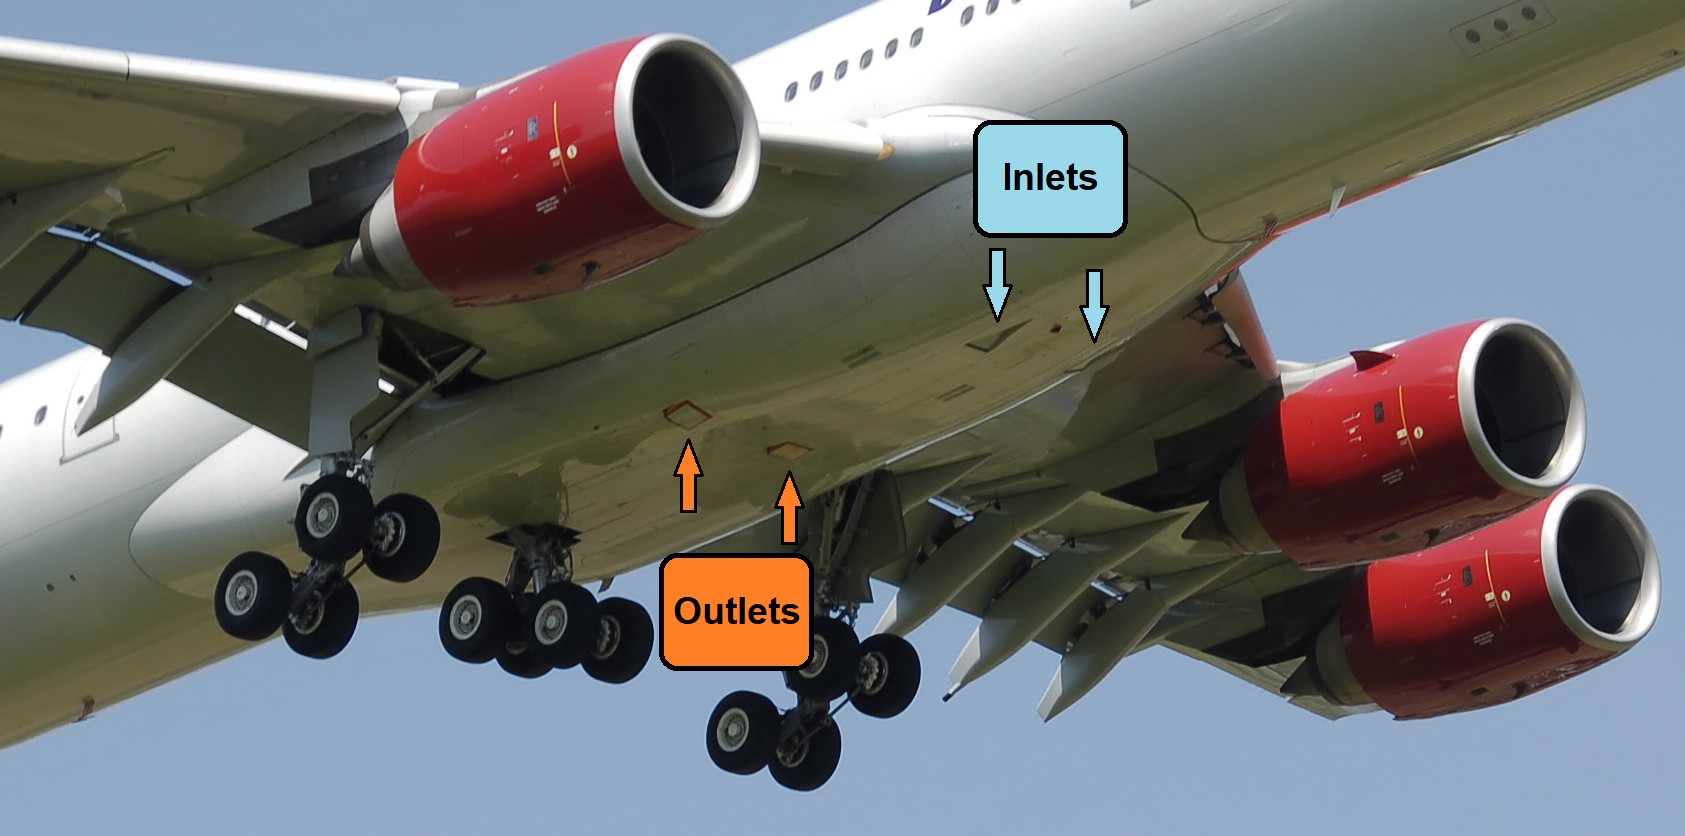
\includegraphics[width=1\textwidth]{Epictures/ECS_Packs_A340-600_Inlet_Outlet.png}
    \caption{Airbus A340-600 two ECS packs in the wing-body fairing with adjustable inlets and outlets for cooling air. Amended from Wikipedia.}
    \label{fig:A340ECS}
\end{figure}

Three different types of \acrshort{ecs}-packs will be laid out:

\begin{enumerate}
\item The conventional, bleed-air driven, Air Cycle Machine (\acrshort{acm}).
\item The Electrical Air Cycle Machine (\acrshort{eacm}).
\item The Electrical Vapour Cycle Machine (\acrshort{evcm}).
\end{enumerate} 

\subsection{Conventional Air Cycle Machine (ACM)}
\label{subsec:ConvACM}
The conventional Air Cycle Machine (\acrshort{acm}), see figure \ref{fig:ACM}, which is most commonly used, is driven by compressed air, called bleed-air, taken from the compressor stages in the engine core. The bleed-air, provide power to run the \acrshort{acm} and air for the cabin. Using the passing through air as a refrigerant, with a combination of turbine, compressors, valves, heat exchangers and outside air to dispense heat, the hot and compressed air can be cooled down well below freezing conditions.

\begin{figure}[!ht]
    \centering
    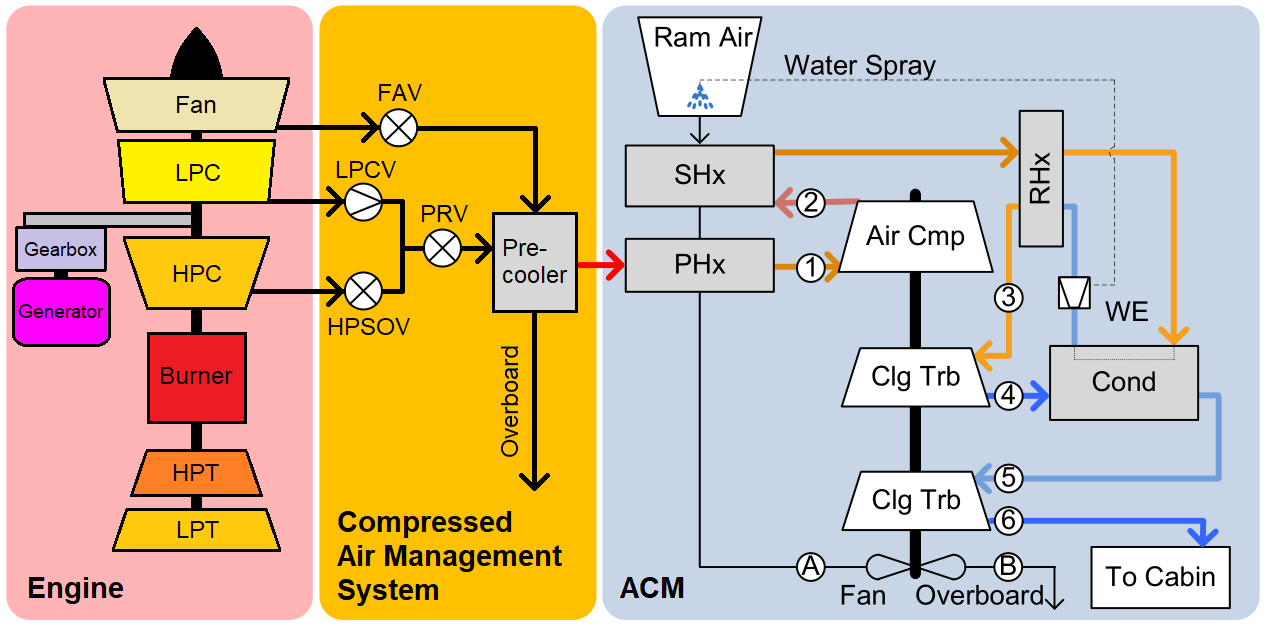
\includegraphics[width=1\textwidth]{Epictures/Pneumatic Bootstrap Four-Wheel Condensing ACM.png}
    \caption{Pneumatic Four-Wheel Condensing Air Cycle Machine. Amended from Parrilla, 2014, \cite{Parrilla2014}.}
    \label{fig:ACM}
\end{figure}

Pressure and temperature of the bleed-air varies with thrust setting of the engine. An engine that is working hard gives bleed-air with high pressure and temperature. Here, the bleed-air can be tapped at either the Low Pressure Compressor (\acrshort{lpc}) or at the High Pressure Compressor (\acrshort{hpc}), depending on   which port that can deliver just enough pressure to drive the \acrshort{acm}. Most of the time, when thrust is on a moderate level, bleed-air is tapped from the \acrshort{hpc}. During short periods of time with high thrust setting, such as during takeoff, bleed-air is taken from the \acrshort{lpc}. A Pressure Regulator Valve, \acrshort{prv}, is used the reduce the pressure to approximately 200 kPa.

Typical bleed-air temperature for the simulated A320 is around 260 \degree C during cruise and at maximum around 340 \degree C during climb, which corresponds to bleed-air pressures around 400 kPa and 800 kPa respectively. For safety reasons, the bleed-air is cooled down below autoignition temperature (200 \degree C) of jet fuel, before it leaves the engine. Heat is dumped overboard with compressed air from the engine fan through the pre-cooler.

Before entering the Air Cycle Machine, the relatively hot airflow through a catalytic converter that breaks down ozone. Air enters the \acrshort{acm} through the Primary Heat Exchanger, \acrshort{phx}, then it is compressed. The heat is squeezed out and discarded through the Second Heat Exchanger, \acrshort{shx}. To prevent ice build-up in the system, moisture must be extracted from the air. To do this, some heat in the air is stored in the Reheat Heat Exchanger, \acrshort{rhx}. While further cooling is done in the Condenser, droplets of water forms and gets expelled in the Water Extractor, \acrshort{we}. Extracted water can then be used to spray over the Secondary Heat Exchanger to increase its effectiveness. The dry and cold air can now regain the heat that has been stored earlier in the \acrshort{rhx}. Finally, the air is expanded through a couple of Cooling Turbines, Clg Trb. The expansion extracts power from the compressed air to drive the \acrshort{acm}. After this stage, the temperature of the air can be as low as -18 \degree C.

To adjust the air temperature, hot air can be taken directly after the \acrshort{phx}, at point 1, through a bypass valve and is joined at point 6, where hot and cold air are mixed together. With this adjustment, the air from the \acrshort{acm} can have a temperature from -14 \degree C to 120 \degree C (Merzvinskas et al., 2020, \cite{Merzvinskas2020}). Before flowing to the cabin, fresh air from the \acrshort{acm} is mixed with recirculated air from the cabin. The mixing ratio is typical 50\% fresh air and 50\% recirculated air. A \acrshort{hepa}-type filter is used to capture most particles, bacteria, and viruses in the recirculated air. The fresh, clean air then makes its way to the cabin through the distribution network, and by the time it enters the cabin, its temperature can vary between 4 \degree C and 71 \degree C.

Air pressure in the cabin is maintained and regulated through one or two Out-Flow Valves, OFV, located at the bottom rear of the fuselage.

\subsection{Electric Air Cycle Machine (E-ACM)}
\label{subsec:EACM}
Taking the Conventional Air Cycle Machine, replace the bleed-air with pressurized air from electrically driven compressors, we get the Electric Air Cycle Machine (\acrshort{eacm}), see figure \ref{fig:E-ACM}. The main advantage over the bleed version is improved control over the pressure of the compressed air, as it is not relying on the thrust setting of the engine. Just enough pressure is produced to drive the \acrshort{acm}, about 100 kPa above cabin pressure.

\begin{figure}[!ht]
    \centering
    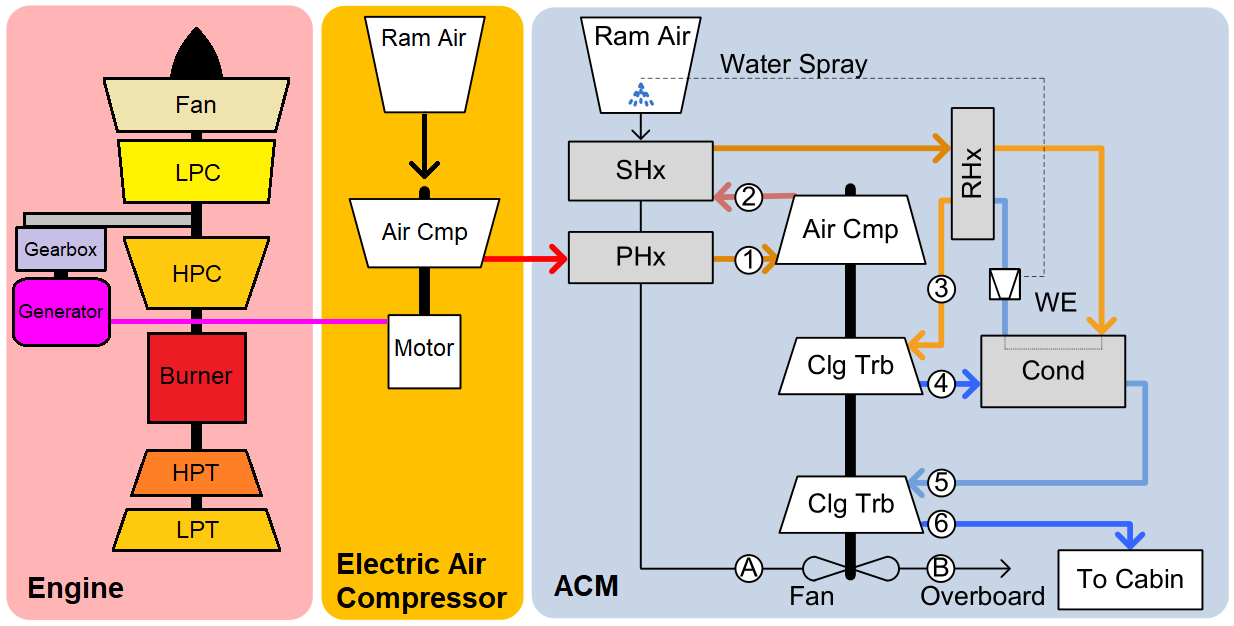
\includegraphics[width=1\textwidth]{Epictures/All Electric Four-Wheel Condensing ECS.png}
    \caption{Electric Four-Wheel Condensing Air Cycle Machine. Amended from Parrilla, 2014, \cite{Parrilla2014}.}
    \label{fig:E-ACM}
\end{figure}


\subsection{Electric Vapour Cycle Machine (E-VCM)}
\label{subsec:EVCM}

The working fluid in the Electric Vapour Cycle Machine, \acrshort{evcm} or even shorter \acrshort{vcm}, is a refrigerant with greater thermodynamic properties than air. This means that the \acrshort{vcm} is more efficient at cooling than the \acrshort{acm}. See figure \ref{fig:E-VCM}. Fresh air for the cabin must still be compressed, but at a lower pressure, around 20 kPa above the cabin pressure. Thus less heat must be extracted and less power is required. Though, the \acrshort{evcm} is more energy efficient than \acrshort{eacm}, the fuel savings may not make up for other disadvantages, such as lower reliability and higher maintenance requirements.

\begin{figure}[!ht]
    \centering
    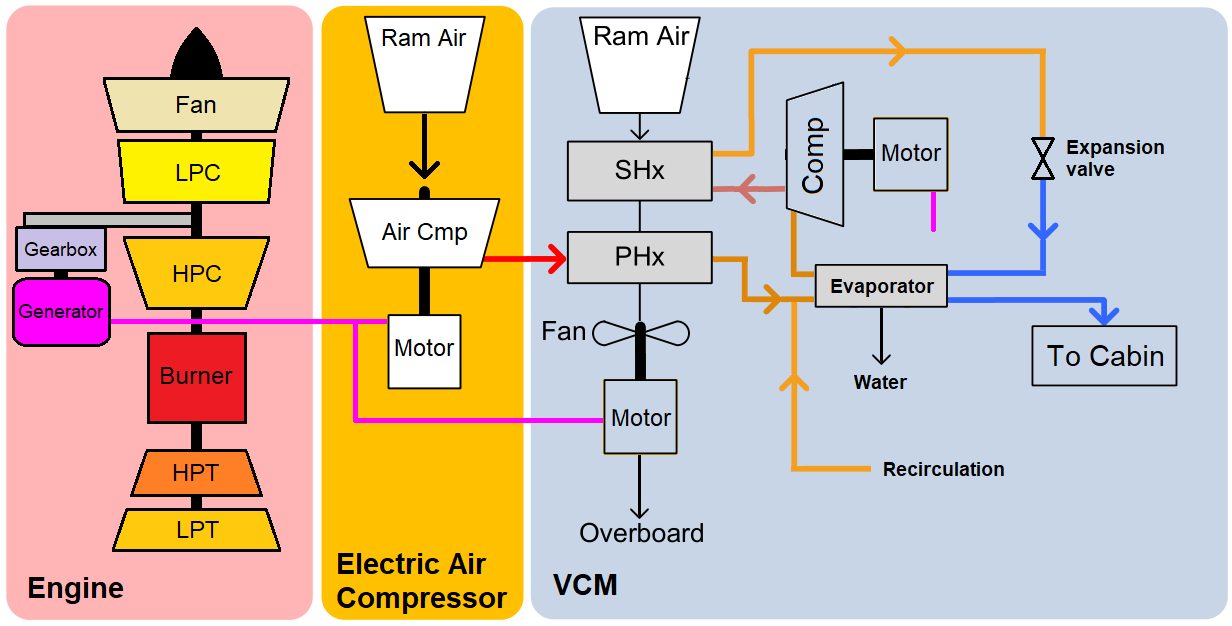
\includegraphics[width=1\textwidth]{Epictures/All Electric VCM ECS.png}
    \caption{Electric Vapour Cycle Machine. Amended from Parrilla, 2014, \cite{Parrilla2014}.}
    \label{fig:E-VCM}
\end{figure}

\section{ECS Thermodynamics}
\label{sec:ECSthermodynamics}

\todo[inline, backgroundcolor=aqua]{Describe the thermodynamics for all 3 ECS variants. Energy balance.}
\todo[inline, backgroundcolor=aqua]{What affects power consumption. Internal and external thermal loads. All assumed parameters.}
\todo[inline, backgroundcolor=aqua]{bleed-air mass flow rate. Dependence of bleed temperature.}
\todo[inline, backgroundcolor=aqua]{Include picture.}

The most important parts of the thermodynamic of this model will be shown here in this chapter. How the model works in detail, can be seen in the Appendix \ref{sec:AppMatlab}, where the MATLAB code is shown.
The control volume of the thermodynamic model is the fuselage of the airliner. It is approximated as a cylinder with an effective length and diameter. The size of the fuselage is a function of pax. The thermal conductivity of the fuselage skin is assumed to have an average value of 5 W/m\textsuperscript{2}K (Chakraborty et al., 2016, \cite{Chakraborty2016}). There are three ways for the heat to flow in and out of the cabin: through fresh air from the \acrshort{ecs}, through the fuselage skin and internal heat generation.


\subsection{Conventional Air Cycle Machine Thermodynamics}
\label{subsec:ConvACMThermodynamics}

 To maintain a cabin temperature of 295.15 K (22 \degree C) under various conditions, the \acrshort{ecs} will initially adjust the temperature of the fresh air. If adjusting the fresh air temperature is not enough, then the airflow rate can be increased. According to regulations, the minimum amount of fresh outside air that must enter the cabin is 10 cfm/pax, which is equal to 6 g/paxs at standard sea level.

Thermal equilibrium for a hot day and static on ground can be described
with:

\begin{equation}
\dot{Q}_{ECS} + \dot{Q}_{shadow} + \dot{Q}_{sun} + \dot{Q}_{pax}  = 0
\end{equation}

,where 

\begin{center}
\begin{tabular}{ r l }
 $\dot{Q}_{ECS}$ & heat flux from the \acrshort{ecs}\\ 
 $\dot{Q}_{shadow}$ & heat flux through the fuselage in shadow\\  
 $\dot{Q}_{sun}$ & heat flux through the fuselage in the sun\\
 $\dot{Q}_{pax}$ & passenger associated heat flux
\end{tabular}
\end{center}

Heat flux from the \acrshort{ecs} can be defined as:

\begin{equation}
\label{eq:QECS}
\dot{Q}_{ECS} = \dot{m}_{air} C_p (T_{ECS} - T_{cabin})
\end{equation}

, where $\dot{m}_{air}$ is the air mass flow rate, $C_p$ is specific heat capacity of air, $T_{ECS}$ is air temperature provided by the \acrshort{ecs} and $T_{cabin}$ is cabin temperature.

Heat flux through the part of fuselage, that is in shadow, from ambient
air is:

\begin{equation}
\dot{Q}_{shadow} = U(A_{wet} - A_{proj})(T_{amb} - T_{cabin})
\end{equation}

, where $U$ is thermal conductivity of fuselage skin, $A_{wet}$ is wet surface area of the fuselage, $A_{proj}$ is projected area of the fuselage, $T_{amb}$ is ambient temperature and $T_{cabin}$ is cabin temperature.

Heat flux through the part of fuselage, that is in the sun can be expressed as:

\begin{equation}
\dot{Q}_{sun} = U A_{proj} (T_{amb} + \Delta T_{solar} - T_{cabin})
\end{equation}

, where $\Delta T_{solar}$ is the average temperature rise of the surface, due to solar radiation. The temperature rise is approximately 10 K (Cottony et al, 1941), for a white surface.

The passenger associated heat flux, $\dot{Q}_{pax}$, is based on metabolic heat and all other facilities such as entertainment, lighting, galley etc. It is roughly 190 W/pax (Slingerland et al. \cite{Slingerland2007}).

\subsubsection{Fresh Air Mass Flow Rate}
\label{subsubsec:ACMair}

Solving for the air mass flow rate, for on ground conditions, gives:

\begin{equation}
\label{eq:mairstatic}
\dot{m}_{air,static} = \frac{U (A_{wet} - A_{proj}) (T_{amb} - T_{cabin}) + U \cdot A_{proj} (T_{amb} + \Delta T_{solar} - T_{cabin}) + \dot{Q}_{pax}}{C_p (T_{cabin} - T_{inlet})}
\end{equation}

, where cooling is assumed with $T_{inlet}=259.37$ K (-13.8 \degree C), for a hot day.

When flying, assume that forced convection will remove most of the solar heating. The temperature rise due to solar heating will then be relatively small and can be neglected. The ambient temperature, $T_{amb}$, is replaced with total temperature, $T_{total}$, to include the kinetic heating effect, thus the air mass flow rate can be calculated as:

\begin{equation}
\label{eq:mairfly}
\dot{m}_{air,fly} = \frac{U \cdot A_{wet} (T_{total} - T_{cabin}) + \dot{Q}_{pax}}{C_p (T_{cabin} - T_{inlet})}
\end{equation}

If heating is required (if eq. \ref{eq:mairstatic} or \ref{eq:mairfly} gives negative value), then assume heating with $T_{inlet}=393.15$ K (120 \degree C).

Ensure that the fresh air mass flow rate meets the regulation. If the calculated air mass flow rate is smaller than the minimum value, $\dot{m}_{air,min}=0.006 \cdot pax$ kg/s, then set $\dot{m}_{air}=\dot{m}_{air,min}$.

With regulated air mass flow rate, a new inlet temperature must be calculated:
%Tinlet = Tc - (Uskin*Awet*(Ttot - Tc) + qpax*pax) / (Cp*bleed_ecs_min); % [K] Throttled ACM to regulate inlet temperature.
\begin{equation}
\label{eq:ACMTinlet}
T_{inlet} = T_{cabin} - \frac{U \cdot A_{wet} (T_{tot}-T_{cabin}) + \dot{Q}_{pax}}{C_p \dot{m}_{air,min}}
\end{equation}

\subsubsection{Heat Exchangers}
\label{subsubsec:ACMHx}
Excessive heat is expelled through the pre-cooler and heat exchangers in the ACM.
The air mass flow rate through a heat exchanger is calculated with the simple assumption that the difference of temperature between the hot air inlet and the cold air outlet is $\Delta T_{hx}$. Further, assume adiabatic process that no heat is transferred to the environment, except between the air in the heat exchanger itself.
If cooling of bleed-air is needed ($T_{bleed}>T_{safe}$), then the fraction of fan air and bleed-air mass flow rate can be expressed as:
%fhxi = (Tbleed-Tsafe)/(Tbleed-1-Tfan);
\begin{equation}
\label{eq:FanXi}
\xi_{fan} = \frac{\dot{m}_{fan}}{\dot{m}_{air}} = \frac{T_{bleed}-T_{safe}}{(T_{bleed}-\Delta T_{hx})-T_{fan}}
\end{equation}
, otherwise $\xi_{fan}=0$.


The fraction of cooling air flow through the heat exchangers in the ACM is expressed as:

\begin{equation}
\label{eq:ACMHx}
\xi_{hx} = \frac{\dot{m}_{hx}}{\dot{m}_{air}} = \frac{T_{safe}-T_{shx}}{(T_{safe}-\Delta T_{hx})-T_{tot}}
\end{equation}



\subsubsection{Conventional Air Cycle Machine Shaft Power}
\label{subsubsec:ACMShaftPower}

For bleed-air, shaft power is a function of air mass flow rate and bleed temperature. According to (Slingerland et al., 2007, \cite{Slingerland2007}) the amount of exergy (in this case, shaft power), extracted from the engine, can be calculated by using:

\begin{equation}
\label{eq:Exergy}
Exergy = P_{shaft} = \dot{m}_{air} \left[ (h-h_0) + T_0 \cdot (s-s_0) \right]
\end{equation}

,where 

\begin{center}
\begin{tabular}{ r l }
 $P_{shaft}$ & shaft power \\ 
 $\dot{m}_{air}$ & bleed-air mass flow rate\\  
 $h$ & enthalpy of bleed-air \\
 $h_0$ & enthalpy of air at compressor inlet \\
 $T_0$ & temperature at compressor inlet \\
 $s$ & entropy of bleed-air \\
 $s_0$ & entropy of air at compressor inlet
\end{tabular}
\end{center}

Enthalpy and entropy can be obtained from data tables when all the temperatures are known. The compressor inlet temperature is the total temperature (static + kinetic), while the compressor outlet temperature is the same as bleed temperature.

When the Auxiliary Power Unit (APU) is providing bleed-air, the bleed-air temperature is:

\begin{equation}
\label{eq:Tapu}
T_{bleed} = T_{total} \cdot 1.258
\end{equation}

, assuming that the pressure ratio is 2, and the compressor efficiency is 0.85.
When the engines are running, the bleed temperature will be set by the engines and various conditions. Details about engine bleed and fan temperature are presented in chapter \ref{ch:bleedtemp}.

The shaft power for the conventional ACM is a sum of 3 different terms, shaft power for fresh air (bleed-air), shaft power for pre-cooler (bleed-air from engine fan) and shaft power for electric circulation fans:

\begin{equation}
\label{eq:ShaftPowerACM}
P_{shaft,ACM} = P_{shaft,bleed} + P_{shaft,fan} + P_{shaft,cf}
\end{equation}

With help from eq. \ref{eq:Exergy} we can express these terms as:

\begin{equation}
P_{shaft,bleed} = \dot{m}_{air}[(h_{bleed}-h_{tot})+T_{tot}(s_{bleed}-s_{tot})]
\end{equation}

\begin{equation}
P_{shaft,fan} = \xi_{fan}\dot{m}_{air}[(h_{fan}-h_{tot})+T_{tot}(s_{fan}-s_{tot})]
\end{equation}

\begin{equation}
\label{eq:cfShaftPower}
P_{shaft,cf} = \frac{P_{cf}}{\eta_{gbx}\cdot\eta_{gen}\cdot\eta_{trn}\cdot\eta_{mot}}
\end{equation}

, where $P_{cf}$ is the power for electric circulation fans, $\eta_{gbx}$ is the gearbox efficiency, $\eta_{gen}$ is the generator efficiency, $\eta_{trn}$ is the transfer efficiency of electricity and $\eta_{mot}$ is the motor efficiency.


\subsection{Electric Air Cycle Machine Thermodynamics}
\label{subsec:EACMThermodynamics}

The thermodynamic model for the conventional and Electric Air Cycle Machine (E-ACM) is the same, only difference is the source of compressed air and the shaft power calculation, since the power is taking a different path from the engine.

Beginning with the supply of compressed fresh air from the electrical compressor. The fresh air mass flow rate is the same as in previous case. The supply pressure is about 100 kPa above cabin pressure. The pressure ratio for the supply air is then:
%EACM_rcomp = (cab_press+100e3)/Ptot; % [1] Compression ratio. Minimum pressure requirement of ACM ECS is around 200e3 Pa, p.9, Martinez, 2020
\begin{equation}
\pi_{comp} = \frac{P_{cabin}+100 \text{ kPa}}{P_{tot}}
\end{equation}

Depending on flight condition and compressor efficiency, the compressed air temperature can be expressed as:

\begin{equation}
\label{eq:Tcomp}
T_{comp} = T_{tot} \left[ 1+\frac{\pi_{comp}^{\frac{\gamma-1}{\gamma}} - 1}{\eta_{comp}} \right]
\end{equation}

, where $\pi_{comp}$ is the pressure ratio, $\gamma = \frac{C_p}{C_v}$ is the ratio of specific heat for air. It changes with temperature but can be approximated to $\gamma \approx 1.4$ in this case. $\eta_{comp}$ is the compressor efficiency.



\subsubsection{Heat Exchangers}
\label{subsubsec:EACMHx}
With the same precedure as with the conventional ACM, the cooling air mass flow rate through the heat exchangers is calculated as:
%erhxi = (EACM_Tcomp-Tshx)/(EACM_Tcomp-dTx-Ttot);
\begin{equation}
\label{eq:ECMHx}
\xi_{hx} = \frac{\dot{m}_{hx}}{\dot{m}_{air}} = \frac{T_{comp}-T_{shx}}{(T_{comp}-\Delta T_{hx})-T_{tot}}
\end{equation}

\subsubsection{Electric Air Cycle Machine Shaft Power}
\label{subsubsec:EACMShaftPower}

With help from eq. \ref{eq:Exergy} , the compressor power can be calculated as:
% EACM_Pcomp = bleed_ecs*1000*((pchip(T,h,EACM_Tcomp)-pchip(T,h,Ttot)) + Ttot*((pchip(T,s,EACM_Tcomp)-pchip(T,s,Ttot))));
\begin{equation}
\label{eq:EACMPcomp}
P_{comp} = \dot{m}_{air} \left[ (h_{comp}-h_{tot}) + T_{tot} (s_{comp}-s_{tot}) \right]
\end{equation}

This power comes from the engine shaft, through a gearbox, a generator, cables, power converters and a motor, all having an efficiency less than unity. Finally shaft power, that is extracted from the engine to the compressor and for the E-ACM, can be calculated:
% shaftpower_EACM_ecs = (EACM_Pcomp + (mode~=0)*ECS_Circfan)/(eta_gbx*eta_gen*eta_mot*eta_trn);
\begin{equation}
\label{eq:Pshaftcomp}
P_{shaft,comp} = \frac{P_{comp}}{\eta_{gbx} \cdot \eta_{gen} \cdot \eta_{cpc} \cdot \eta_{mot}}
\end{equation}

\begin{equation}
\label{eq:EACMPshaft}
P_{shaft,EACM} = P_{shaft,comp} + P_{shaft,cf}
\end{equation}

, where shaft power for the circulation fans, $P_{shaft,cf}$, is the same as in eq. \ref{eq:cfShaftPower}.

\subsection{Electric Vapour Cycle Machine Thermodynamics}
\label{subsec:EVCMThermodynamics}

Like the \acrshort{eacm}, \acrshort{evcm} also uses an electric air compressor to deliver air to the cabin, but at a lower pressure, since the pressurized air is not used to drive the machine, as for the \acrshort{acm}. The air mass flow rate is the same as for the \acrshort{acm}.

The supply pressure is about 20 kPa above cabin pressure. The pressure ratio for the supply air is then:
%VCM_rcomp = (cab_press+20e3)/Ptot; % [1] Compression ratio. Minimum pressure requirement of VCM ECS is 120e3 Pa, p.16, Martinez,2020
\begin{equation}
\pi_{comp} = \frac{P_{cabin}+20 \text{ kPa}}{P_{tot}}
\end{equation}

The compressed air temperature,$T_{comp}$, is calculated as in eq. \ref{eq:Tcomp}.



\subsubsection{VCM Operation}
\label{subsubsec:EVCMOperation}
Since the fresh compressed air temperature is not as high as for the previous machines, cooling through heat exchangers is not always necessary. Often, heat exchangers must be throttled or even turned off. In extremely cold conditions, such as cruising at high altitudes, the electric heater is most likely to add additional heat to the cabin.

The fresh air mass flow rate and inlet temperature are the same for the \acrshort{vcm} as for the previous machines, since they are all simulated with the same aircraft model.
%We begin with the supply air temperature for the cabin. When the speed is low and the solar heating effect must be considered, then the supply air temperature for the cabin can be expressed as:
% VCM_Tinlet = Tc - (Uskin*(Awet - Aprj)*(Ttot - Tc) + Uskin*Aprj*(Ttot + Tsolar - Tc) + qpax*pax) / (Cp*bleed_ecs_min); % [K] Required inlet temperature for equilibrium.
%\begin{equation}
%\label{VCMTinletog}
%T_{inlet} = T_{cabin} - \frac{U(A_{wet}-A_{prj})(T_{tot}-T_{cabin}) + U\cdot %A_{prj}(T_{tot}+\Delta T_{solar} - T_c) + \dot{Q}_{pax}}{C_p \dot{m}_{air,min}}
%\end{equation}

%When flying, the solar heating effect is neglected and we get:
% VCM_Tinlet = Tc - (Uskin*Awet*(Ttot - Tc) + qpax*pax) / (Cp*bleed_ecs_min); % [K] Required inlet temperature for equilibrium.
%\begin{equation}
%\label{VCMTinletfly}
%T_{inlet} = T_{cabin} - \frac{U A_{wet}(T_{tot}-T_{cabin}) + \dot{Q}_{pax}}{C_p %\dot{m}_{air,min}}
%\end{equation}

If cooling is needed by the Vapour Cycle Machine, then the cooling effect is expressed as:
% Hvcm = bleed_ecs_min*Cp*(Ttot+dTx-VCM_Tinlet); % [W] Heat that needs to be extracted by the VCM.
\begin{equation}
\label{VCMQ}
\dot{Q}_{VCM} = \dot{m}_{air}C_p((T_{tot}+\Delta T_{hx})-T_{inlet})
\end{equation}

The power to run the vapour cycle compressor is calculated as:
%VCM_Pref = Hvcm/COPr; % [W] VCM compressor power for cooling.
\begin{equation}
\label{VCMPref}
P_{comp,VCM} = \frac{\dot{Q}_{VCM}}{\text{COP\textsubscript{R}}}
\end{equation}

Coefficient of Performance Refrigerator (COP\textsubscript{R}) can vary depending on temperatures and refrigerant but be set to 3, for simplicity. This means that 1 kW of power input to the VCM motor can pull out 3 kW of heat from the system.


The cooling air mass flow rate through the primary heat exchangers is:
% m_phx = bleed_ecs_min*(VCM_Tcomp-(Ttot+dTx))/(VCM_Tcomp-dTx-Ttot); % [kg/s] Cooling air mass flow rate through primary heat exchanger.
% m_shx = Hvcm*(1+1/COPr)/(Cp*(Tshx-Ttot)); % [kg/s] Cooling air mass flow rate through secondary heat exchanger.
\begin{equation}
\label{VCMphx}
\dot{m}_{phx} = \dot{m}_{air}\frac{T_{comp}-(T_{tot}+\Delta T_{hx})}{(T_{comp}-\Delta T_{hx})-T_{tot}} = \dot{m}_{air}
\end{equation}

While the cooling air mass flow rate through the secondary heat exchangers is:

\begin{equation}
\label{VCMshx}
\dot{m}_{shx} = \frac{\dot{Q}_{VCM}(1+1/COP_r)}{C_p (T_{shx}-T_{tot})}
\end{equation}



If no cooling is required, then the vapour cycle compressor is turned off, $P_{comp,VCM}=0$ and as a consequence, there is no cooling airflow through the secondary heat exchanger, $\dot{m}_{shx}=0$.
% VCM_Pref = 0; % [W] VCM compressor power off.
% m_shx = 0; % [kg/s] Cooling air mass flow rate through secondary heat exchanger not needed.


Cooling air mass flow rate through the primary heat exchanger is throttled according to:
% m_phx = bleed_ecs_min*(VCM_Tcomp-VCM_Tinlet)/(VCM_Tcomp-dTx-Ttot); % [kg/s] Cooling air mass flow rate through primary heat exchanger.
\begin{equation}
\label{VCMphxThrottled}
\dot{m}_{phx} = \dot{m}_{air} \frac{T_{comp}-T_{inlet}}{(T_{comp}-\Delta T_{hx})-T_{tot}}
\end{equation}

If heating is needed, then primary heat exchanger is turned off, $\dot{m}_{phx}=0$, and the electric heater is turned on with a power of:
% if m_phx < 0 % Cabin need more heat than what the compressed air can provide.
%   VCM_Peh = -Uskin*Awet*(Ttot - Tc) - bleed_ecs_min*Cp*(VCM_Tcomp-Tc) - qpax*pax; % [W] Electric heater
%   m_phx = 0; % [kg/s] Turn off cooling air flow
%  end
\begin{equation}
\label{VCMPeh}
P_{eh} = -U\cdot A_{wet} (T_{tot}-T_{cabin}) - \dot{m}_{air} C_p (T_{comp}-T_{cabin}) - \dot{Q}_{pax}
\end{equation}


\subsubsection{Electric Vapour Cycle Machine Shaft Power}
\label{subsubsec:EVCMShaftPower}
Power to compress supply air is expressed as:
%VCM_Pcomp = bleed_ecs_min*1000*((pchip(T,h,VCM_Tcomp)-pchip(T,h,Ttot)) + Ttot*((pchip(T,s,VCM_Tcomp)-pchip(T,s,Ttot))));
\begin{equation}
\label{eq:EVCMPcomp}
P_{comp} = \dot{m}_{air} \cdot \left[ (h_{comp}-h_{tot}) + T_{tot} \cdot (s_{comp}-s_{tot}) \right]
\end{equation}

The total shaft power to run the E-VCM is:
% Shaft power due to Compressor, VCM, HX-fan , Electric heater and
% circulation fans.
% shaftpower_VCM_ecs = (mode~=0)*(VCM_Pcomp + ECS_Circfan + VCM_Pref + VCM_hxfan) / %(eta_gbx*eta_gen*eta_mot*eta_trn) + VCM_Peh/(eta_gen*eta_gbx*eta_trn);
\begin{equation}
\label{eq:EVCMPshaft}
P_{shaft,EVCM} = \frac{P_{comp} + P_{comp,VCM} + P_{cf} +  P_{hxf}}{\eta_{gbx} \cdot \eta_{gen} \cdot \eta_{trn} \cdot \eta_{mot}} + \frac{P_{eh}}{\eta_{gbx} \cdot \eta_{gen} \cdot \eta_{trn}}
\end{equation}

,where power for the circulation fans ,$P_{cf}$, is the same as for the conventional ACM. Power to pull cooling air through the heat exchangers is $P_{hxf}$.

\section{ECS Weight Impact}
\label{sec:ECSweight}

%\todo[inline, backgroundcolor=aqua]{Show the weight for all 3 ECS variants.}
%\todo[inline, backgroundcolor=aqua]{Describe how weight differences affect fuel consumption %through L/D ratio and TSFC.}

The weight of the \acrshort{ecs} contributes to fuel consumption through Lift-to-Drag ratio of the aircraft. Increased weight leads to increased drag, while drag transforms to fuel consumption by the engines' Thrust Specific Fuel Consumption (\acrshort{tsfc}).

The mass of the \acrshort{ecs} is a function of technology and rated power. Therefore Specific Power (\acrshort{sp}) is chosen to distinguish different technologies. For the conventional ACM, bleed-air mass flow rate is chosen instead of power.

The specific power is used in the simulation to estimate \acrshort{ecs} mass according to:

\begin{equation}
\label{eq:ECSmass}
m_{ECS} = \frac{RP}{SP}
\end{equation}

The rated power, \acrshort{rp}, is a function of passenger count, pax, and data from several airliners with different sizes.\\

According to Tagge et al., 1985, \cite{Tagge1985}, environmental control system modi-fications from the Baseline, 197 pax airliner with 2 engines, bleed-air \acrshort{ecs} to a no-bleed electric \acrshort{ecs} results in additional system mass, despite the removal of bleed associated ducting, valves and pre-coolers. See table \ref{table:TaggeMass}. It is assumed that mass increase, associated with higher electric power demand by the \acrshort{ecs}, also includes more powerful generators and transfer systems.

%Baseline uses bleed fed air cycle machines, weights 1034 kg and is probably rated for 2 kg/s of bleed-air. Then the bleed mass-to-weight ratio for conventional ECS is about $1.93 \cdot 10 ^{-3} [\frac{kg/s}{kg}]$.

%Configuration E-ACM, which uses electric compressors with heat exchangers and air cycle machines, has 0.171 kW/kg.
%Configuration E-VCM, which uses electric compressors with heat exchangers and vapour cycle machines, has 0.124 kW/kg.
%Configuration 4, the same as E-ACM but without heat exchangers, has0.194 kW/kg.

\begin{table}[h!]
\centering
\caption{ECS mass and specific power for a 197 pax airliner. Amended from Tagge et al. 1985, \cite{Tagge1985}}
\begin{tabular}{| c | c | c | c |} 
\hline
Technology & Connected Power & Mass & Specific Power \\
\hline
Bleed ACM & 2.00 kg/s & 1034 kg & $1.93 \cdot 10 ^{-3}$ (kg/s)/kg \\
Electric ACM & 262.5 kW & 1533 kg & 0.171 kW/kg \\
Electric VCM & 202.8 kW & 1633 kg & 0.124 kW/kg \\
\hline
\end{tabular}
\label{table:TaggeMass}
\end{table}

As described by Martinez, 2020, \cite{Martinez2020}, we can read about the conventional \acrshort{ecs} for the A320 (180 pax) and the A340 (400 pax). The A320 has 2 ACM packs and are rated for 2 kg/s of bleed-air. The A340 has 4 ACMs, while they are rated for 4 kg/s of bleed-air. The \acrshort{ecs} for the A340 weighs 720 kg, which means 180 kg/pack. Martinez further describes that larger airliners usually have 1 pack per engine, each rated for 1 kg/s of bleed-air and weighs some 150 kg each. Note that mass presented here do not include the mass of bleed valves, pre-coolers and ducts. Thus we can not use these numbers for the \acrshort{ecs} as a whole system.

Berlowitz, 2010, \cite{Berlowitz2010}, described mass changes when fitting a couple of Wide-Body twin-engine airliners, about the same size as the A340, with electric instead of bleed ACM. See table \ref{table:BerlowitzMass}. We can see that the removed pneumatic parts, bleed-air valves, pre-coolers and ducts, weigh around 603 kg. For the A340 the packs mass is 720 kg, then the \acrshort{ecs} mass is 720+603=1323 kg. If the rated bleed-air mass flow rate is 4 kg/s, then the mass-to-weight ratio is $4/1323 \approx 3.02 \cdot 10^{-3} \left[\frac{kg/s}{kg}\right]$. The power-to-weight ratio for the E-ACM can be estimated to 500kW/(1323+97)kg $\approx 0.352$ kW/kg.

We can estimate approximately that the packs have the same mass as the pneumatic components. For the case with the A320, 2 packs weigh 300 kg, then the \acrshort{ecs} mass would be around 600 kg. The bleed mass-to-weight ratio would then be $2/600 \approx 3.33 \cdot 10^{-3} \left[\frac{kg/s}{kg}\right]$.

\begin{table}[h!]
\centering
\caption{ECS mass difference, comparing conventional Air Cycle Machine and the electric counterpart. The ECS is rated for 2x250 kW and is design for A330 and B767, around 400 pax. Amended from Berlowitz, 2010, \cite{Berlowitz2010}}.
\begin{tabular}{| c | c |} 
\hline
Component & Mass difference [kg] \\
\hline
Generators 500 kW & 150 \\
Motors & 150 \\
Controllers & 340 \\
Compressors & 60 \\
Removed pneumatic parts & -603 \\
\hline
Total & 97 \\
\hline
\end{tabular}
\label{table:BerlowitzMass}
\end{table}

According to Chakraborty et al.,2016, \cite{Chakraborty2016}, we can read that the electric architecture add weight to the aircraft, relative to the conventional architecture. See table \ref{table:ChakrabortyMass}. Assume that about 44\%, $\frac{200 \text{kW}}{540 \text{kVA}\cdot 0.85}\approx 0.44$, of the rated power is used for the E-ACM.

\begin{table}[h!]
\caption{Mass penalty by the Electric Air Cycle Machine for A320 sized airliner. Amended from Chakraborty et al.,2016, \cite{Chakraborty2016}}
\centering
\begin{tabular}{| c | c |} 
 \hline
 Component & Mass difference [kg] \\
 \hline
 Air compressors 200 kW & 80\\ 
 Generators 540 kVA & $0.44\cdot(196-87)\approx48$\\
 Additional wiring & $0.44\cdot84=37$\\
 Power electronics & $0.44\cdot130=57$\\
 APU & $0.44\cdot98=43$\\ 
 \hline
 E-ACM weight penalty & 265\\
 \hline
\end{tabular}
\label{table:ChakrabortyMass}
\end{table}

As we saw previously that the conventional \acrshort{ecs} for the A320 weighs about 600 kg. If we would convert to the E-ACM with associated electric architecture, then there would be a mass penalty of 265 kg. The power-to-weight ratio for this E-ACM would then be $\frac{200 \text{kW}}{600+265 \text{kg}}\approx 0.231$ kW/kg.

According to Milewski, 2019, \cite{D.M.N.Milewski2019}, there is a weight penalty when retrofitting an airliner with electric \acrshort{ecs}, not to mention the re-certification time. For the A320, this weight penalty is estimated to be around 400 kg based on currently installed technology on the aircraft. Still, with more advanced technology can be reduced to 200 kg. If we compute the electric \acrshort{ecs} power-to-weight ratio, we get $\frac{200 \text{kW}}{600+200 \text{kg}}= 0.250$ kW/kg.\\

To conclude the specific power of different \acrshort{ecs} technology, we can see that the numbers, provided by Tagge et al., 1985, \cite{Tagge1985}, deviates considerably from the rest. We can also see that the report was written 25-35 years ahead of the rest, so the values from that report will not be used directly, but as a reference to see the development of specific power.

For the other sources an average for the conventional Air Cycle Machine \acrshort{ecs} mass-to-weight ratio is $3.18 \cdot 10 ^{-3} \left[\frac{kg/s}{kg}\right]$.

For the electric Air Cycle Machine \acrshort{ecs}, the average system power-to-weight ratio is 0.278 kW/kg. Boeing B787 uses this system.

No modern studies could be found on the electric \acrshort{ecs} with Vapour Cycle Machine. Still, if we assume the same leap in technology as with the electric Air Cycle Machine, then the power-to-weight ratio for the electric Vapour Cycle Machine \acrshort{ecs} would probably be around 0.202 kW/kg.\\

A summary of \acrshort{ecs} specific power for different technology is shown in table \ref{table:ECSSpecificPower}.

\begin{table}[h!]
\centering
\caption{Summary of ECS specific power.}
\begin{tabular}{| c | c |} 
\hline
Technology & Specific Power \\
\hline
Bleed ACM & $3.18 \cdot 10 ^{-3}$ (kg/s)/kg \\
Electric ACM & 0.278 kW/kg \\
Electric VCM & 0.202 kW/kg \\
\hline
\end{tabular}
\label{table:ECSSpecificPower}
\end{table}


\section{ECS Drag}
\label{sec:ECSdrag}
%\todo[inline, backgroundcolor=aqua]{Describe how intake of fresh air for the cabin and cooling air for the heat exchangers creates drag.}
%\todo[inline, backgroundcolor=aqua]{Connect drag to fuel consumption through TSFC.}
%\todo[inline, backgroundcolor=aqua]{Include picture of air scoops.}

While bleed-air results in shaft power loss, intake of air through scoops creates drag, which can be expressed with Newton's Second Law:
%$$F = \frac{d(m\cdot v)}{dt}$$
\begin{equation}
\label{Newton2Law}
F = \frac{d(m\cdot v)}{dt}
\end{equation}

Drag can directly be converted to fuel consumption by multiplying with \acrshort{tsfc}.

The amount of mass flow rate of air through scoops, $\dot m_{scoops}$, is a sum of cooling air through the heat exchangers and intake of fresh air for the electric \acrshort{ecs}. The air mass flow rate is determined by the \acrshort{ecs}, while airspeed, $v$, is decided by the flight profile. We can formulate the drag as:
%$$D = \dot m \cdot v $$
\begin{equation}
\label{ScoopDrag}
D_{scoops} = \dot m_{scoops} \cdot v 
\end{equation}

Effects of the shape of the air scoops and how they interact with the rest of the aircraft is believed to be small, thus have been neglected.
Figure \ref{fig:A320Scoops} shows the air scoops for the \acrshort{ecs} packs. Their openings can be adjusted to regulate cooling of the heat exchangers in the \acrshort{ecs} packs.

\begin{figure}[!ht]
    \centering
    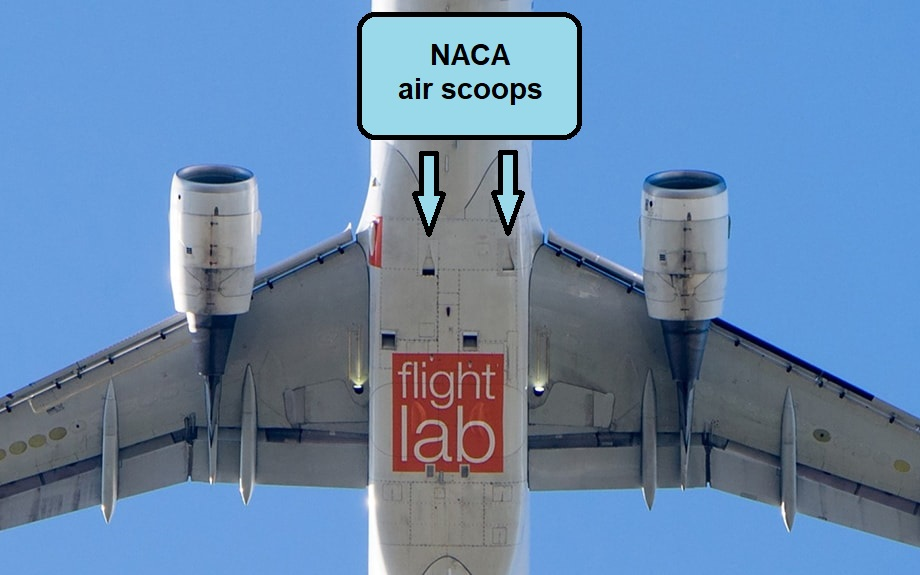
\includegraphics[width=1\textwidth]{Epictures/A320_Scoops_closer.jpg}
    \caption{Airbus A320 with partly open air scoops for the \acrshort{ecs}. Amended from GKN Aerospace, \cite{GKN2020}.}
    \label{fig:A320Scoops}
\end{figure}


\section{ECS Fuel Consumption}
\label{sec:ECSFuelConsumption}

%The ECS can be divided into many sub-assemblies, each with their own ways of consuming power. It can be electric power, mechanical power or pneumatic power. All major power comes from the engines. So it is natural to use shaft power as a common unit, then the step to fuel consumption is not far away.

Fuel consumption of the \acrshort{ecs} is a function of shaft power for bleeding air, shaft power to run the machine, air intake induced drag, and lift induced drag. For the bleed driven \acrshort{ecs}, the engines can even be forced to run at a higher thrust setting than what is needed by the aircraft, then the \acrshort{ecs} should also be accounted for the thrust increased fuel consumption.


Fuel consumption for the general \acrshort{ecs} can be formulated as:
\begin{equation}
\label{ECSFuel}
\dot{m}_{fuel,ECS} = \dot{m}_{fuel,Pshaft} + \dot{m}_{fuel,drag} + \dot{m}_{fuel,mass} + \dot{m}_{fuel,thrust}
\end{equation}

Fuel consumption due to shaft power to run the \acrshort{ecs} is:
\begin{equation}
\label{ECSFuelshaft}
\dot{m}_{fuel,Pshaft} = kp\cdot TSFC \cdot P_{shaft,ECS}
\end{equation}

Fuel consumption by the air scoop drag is:
\begin{equation}
\label{ECSFueldrag}
\dot{m}_{fuel,drag} = TSFC \cdot D_{scoops}
\end{equation}

Fuel consumption induced by mass of the \acrshort{ecs} is:
\begin{equation}
\label{ECSFuelmass}
\dot{m}_{fuel,mass} = TSFC \frac{m_{ECS}\cdot g}{LoD}
\end{equation}

Fuel consumption for the \acrshort{ecs} forced thrust increase is:
\begin{equation}
\label{ECSFuelthrust}
\dot{m}_{fuel,thrust} = TSFC \cdot \Delta T_{ECS}
\end{equation}


\acrshort{kp} is the Shaft Power Factor, $g$ is the gravitational constant, \acrshort{lod} is the Lift-to-Drag ratio and $\Delta T_{ECS}$ is the \acrshort{ecs} forced thrust increase.\\


%########################################################################################
\cleardoublepage
\chapter{Aircraft Icing}
\begin{figure}[!ht]
    \centering
\graphicspath{ {IPS/} }
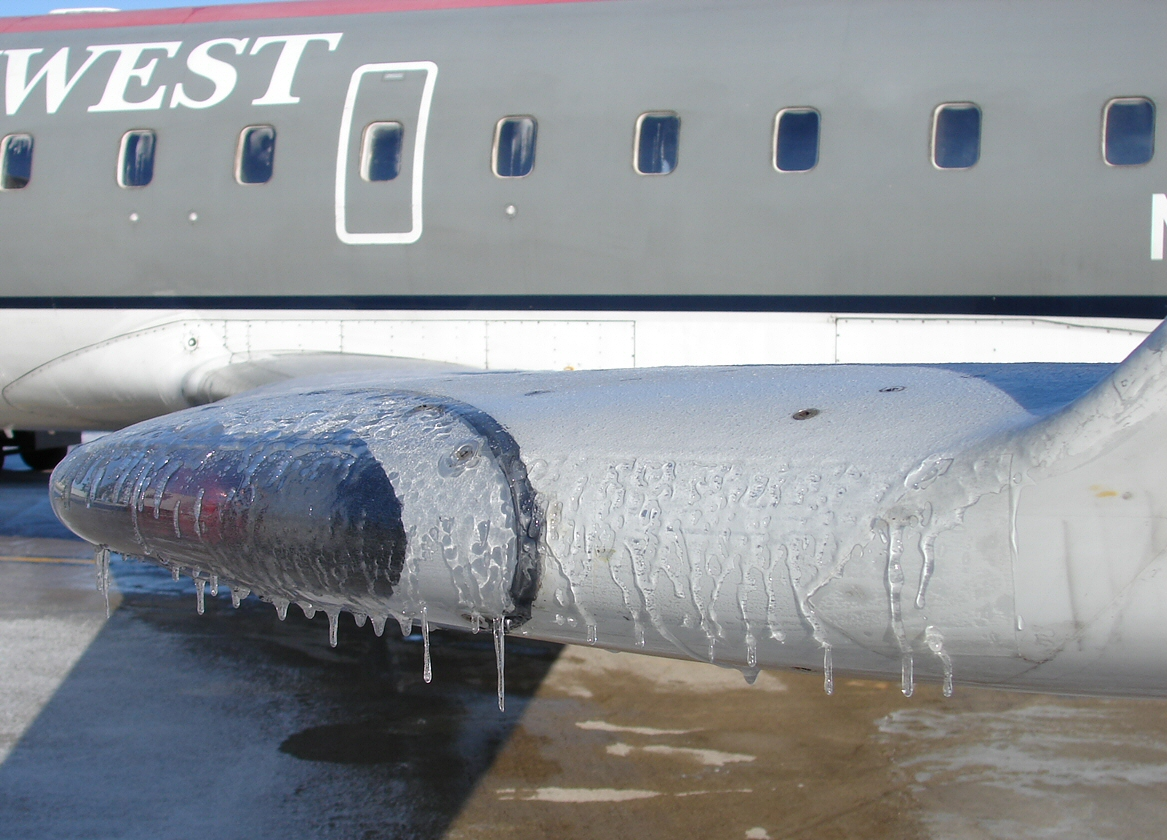
\includegraphics[width=\textwidth,height=\textheight,keepaspectratio]{Ice_on_an_aircraft_wing}
\caption{Ice on an aircraft wing, \cite{icingpic}}
\label{fig:Aircraftice}
\end{figure}
Before we delve deeper into ice protection, we need to understand why icing occurs and how it affects an aircraft. This chapter intends to answer the basics related to icing in aircraft.
\section{Why and where does icing occur?}
\label{sec:whyicingoccurs}
Following factors influence icing in aircraft:
\begin{enumerate}
\item \textbf{Supercooled Large Water Droplets (\acrshort{sld})}: Aircraft undertakes flight through clouds consisting of supercooled droplets that contact the aircraft surface and freeze. The droplets accumulate over time to form an icing layer on the surface. The \acrshort{sld} is divided into two groups of \acrshort{mvd} less than and greater than 40 $\mu$m \cite{EuropeanAviationSafetyAgency2020}.
\item \textbf{Precipitation}: Water droplets from rain or snow freeze on contact with the aircraft surface. When the air temperature lies between 0 \degree C and 3 \degree C , the snow consists of liquid water. This liquid water, in turn, causes the snow crystals to form weak bonds with each other. The weak bonds turn into strong bonds when the air temperature falls below 0 \degree C (Dalili et al, 2009) \cite{Thorsson} \cite{Dalili2009}.
\end{enumerate}

There have been numerous experiments to ascertain the effects of icing in aircraft. We observe that icing affects the aircraft's primary aerodynamic forces, i.e., lift, weight, thrust, and drag. The observable parameters that support this finding are the drag, lift coefficients, and the mass of ice produced. As a consequence, icing poses a significant threat that causes effects such as loss in altitude, airspeed, and lift while at the same time increasing power consumption of other aircraft subsystems.The locations of icing occurrence include leading edges of airfoil, tailgate, cockpit glass, windows, pitot tube, ailerons, antennas and inlet tip of engine nacelles.

\section{Ice Types}
\label{sec:icetypes}
\begin{enumerate}
\item \textbf{Rime Ice} : Rime ice is created when \acrshort{sld} hit the surface of aircraft, and quickly freeze on impact. It has a milky-white and crystalline appearance. The favorable conditions for rime ice include small, supercooled droplets present in stratiform clouds. Airfoil shape and leading edges near the engine inlet are the locations where there is a possibility of rime ice formation. It is formed where there is zero local velocity of the fluid (stagnation point) \cite{WikiIcing}.
\item  \textbf{Glaze/Clear Ice} : It is a thick layer of glass-like ice created while the aircraft is in flight where there is a high availability of \acrshort{sld}. A small part of the droplet hits the surface of the aircraft, and gradually freezes on impact. In some cases, there is uneven distribution of glaze ice throughout the wing surface. The favorable conditions for glaze ice include large droplets present in cumuliform clouds, freezing rain or terrain effects. \cite{icinghazard}
\item \textbf{Mixed Ice}: Mixed ice has both Rime and Glaze ice properties. It has a rugged and opaque appearance. The favorable conditions for mixed ice include the coexistence of large and small droplets, liquid and frozen particles, and wet snow.
\end{enumerate}

\section{Cloud Types}
\label{sec:cloudtypes}
The scope of the study covers Continuous Maximum (CM) Stratiform and Intermittent Maximum (IM) for Cumuliform Clouds.
\begin{enumerate}
\item \textbf{Cumuliform Clouds} : Formed due to severe convection, they are heavy and can hold a high \acrshort{lwc}. The constrained horizontal extent is exposed to the aircraft for a short period.
\item \textbf{Stratus Clouds}: Formed due to less severe convection than Cumuliform Clouds.The stratified layer thus formed covers a wide area. They are not as heavy, however can sometimes hold a high \acrshort{lwc}. Also called as layer clouds. Icing layers are uncommon with a vertical extent of more than 3.000 ft.
\item \textbf{Freezing Rain} : Significant icing happens while the aircraft is flying on cold air mass and below a warm air layer. Raindrops have a larger capture rate than cloud droplets. They form clear ice at freezing temperatures.
\item \textbf{Freezing Drizzle} : Drizzle falls from stratus clouds which have a high \acrshort{lwc}. The drizzle freezes on or close to the contact surface of an object or the ground itself.
\end{enumerate}

\begin{figure}[!ht]
    \centering
\graphicspath{ {IPS/} }
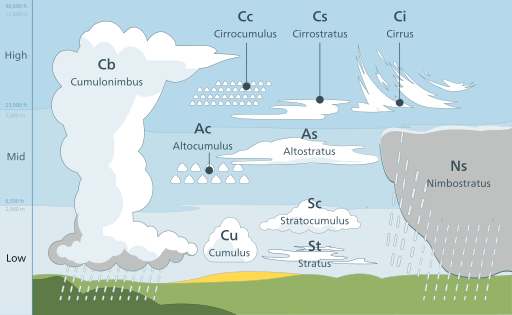
\includegraphics[width=\textwidth,height=\textheight,keepaspectratio]{512px-Cloud_types_en.svg}
\caption{Cloud Types \cite{Habashi2004}}
\label{fig:CloudT}
\end{figure}

\section{Parameters for Icing formation}
\label{sec:iceparameters}
Average droplet size, liquid water content, and the air temperature primarily constitute the deterministic parameters
for the icing conditions. 
\subsection{Drop Median Volumetric Diameter (\acrshort{mvd})}
\label{subsec:medvoldia}
Drop median volumetric or otherwise called as median droplet diameter, refers to the center point droplet size, where half of the amount of the droplet is smaller, and the other half of the droplets is larger than the mean droplet volume. The extent of the aft limit of the \acrshort{ips} is usually calculated with a \SI{40}{\micro\metre} \acrshort{mvd} , as prescribed by \acrshort{faa}. \acrshort{mvd} of \SI{40}{\micro\metre} reveals that half of the volume is less than \SI{40}{\micro\metre} of droplet size, while the other half is more than \SI{40}{\micro\metre}\cite{Heinrich1991}.


\subsection{Droplet Distribution}
\label{subsec:medvoldia}
It is necessary to know the droplets' size to explain and predict icing simulations accurately. Langmuir and Blodgett (1946) proposed a monodisperse droplet distribution in which half of the droplets had a smaller radius and the other half a larger radius in the fog. Monodispersion is a commonly used method and has been chosen as one of the input icing design parameters. Additionally,  Langmuir D distribution is selected as paramater for one of the icing simulation. Figure~\ref{fig:LangmuirD} shows the collection efficiency of droplets under Langmuir D distribution. 

\subsection{Droplet Impingement}
In order to evaluate the thermal inputs for removing ice accumulation, the design of ice protection systems includes awareness of local and total impingement intensities. Experiments have been performed in the past by NASA Glenn Research Center and at the FAA Technical Center. In a typical experiment setup, the data is captured through a Charge Coupled Device Camera. These devices specialize in capturing highly sensitive optical signals. Analysis is typically performed on components such as Finite Wings, Inlets of engines and Airfoils. The droplet distribution is around a \acrshort{mvd} of \SI{16,5}{\micro\metre} and \SI{20,4}{\micro\metre}. Droplet impingement is mathematically characterized by the Collection efficiency. The collection efficiency is the fraction of liquid water in the path of an aircraft component that, when traveling in icing conditions, is accumulated as ice on that component \cite{skybrary}. 


\subsection{Liquid Water Content (\acrshort{lwc})}
\label{subsec:liqwatcon}The \acrshort{lwc} is a parameter which influences the rate of ice accretion, the icing type, and risk of runback water freezing behind the protected areas\cite{dtic}. It is the \textit{liquid water quantity per unit volume of air}. It is calculated from Appendix C, corresponding to \acrshort{mvd}, ambient temperature and pressure altitude for a standard horizontal extent. It is measured in $g/m^3$. The higher the \acrshort{lwc}, the higher the amount of ice accretion.

\subsection{Icing Air Temperature (Ambient Temperature)}
\label{subsec:iceairtemp}
Icing Air temperature is the subzero \degree C temperature corresponding to ice formation. It is measured in \degree C.
\subsection{Horizontal Extent}
The horizonal extent is defined as the extent or height of air mass corresponding to the cloud. It is measured in $nm$. 

\subsection{Vertical Extent}
The vertical extent is defined as the extent or depth of air mass corresponding to the cloud. It is measured in $nm$. 

\section{Icing Standards}
\label{subsec:icestd}
The \acrshort{ips} must certify airworthiness requirements for flights into icing conditions. At present, the safety regulation is pursuant to Appendix C, Amendment 24, CS-25 of European Union Safety Agency (EASA) \textit{ED Decision 2020/001/R}. The primary objective of Appendix C is to provide the highest possible (99\%) icing conditions that the \acrshort{ips} should endure . According to Appendix C Part 1, for a non standard horizontal extent, the \acrshort{lwc} is calculated by multiplying the \acrshort{lwc} values of standard horizontal extent, by the liquid water content factor $F$ corresponding to the non-standard horizontal extent. Appendix O provides the data for calculating the \acrshort{lwc} for a non-standard horizontal extent subject to freezing rain and freezing drizzle conditions.

Subsequently, Appendix O provides \acrshort{sld}, freezing drizzle and freezing rain icing conditions pursuant to Amendment 24, CS-25 of European Union Safety Agency (EASA) \textit{ED Decision 2020/001/R} \cite{EuropeanAviationSafetyAgency2020}.

\subsection{Design Standards}
\label{subsec:desnstd}
Based on the Appendix C, we have the following parameters for continuous maximum or Stratiform clouds:
\begin{enumerate}
\item Cloud \acrshort{lwc}  should be between 0.14 $g/m^3$ and 0.18 $g/m^3$ (for 0 \degree C).
\item The ambient or aircraft surface temperature should be below 0 \degree C.
\item The air temperature should be above -30 \degree C.
\item Maximum vertical extent of 2000 m (6.500 ft).
\item Horizontal extent has a standard value of 17,4 nautical miles, or 32,2 km.
\item Pressure altitude ranges from sea level to 6.700 m (22.000 ft).
\item The \acrshort{mvd} should lie in the range between \SI{15}{\micro\metre} and \SI{40}{\micro\metre}.
\end{enumerate}

Based on the Appendix C, we have the following parameters for intermittent maximum or Cumuliform clouds:
\begin{enumerate}
\item Cloud \acrshort{lwc}  should be between 0.14 $g/m^3$ and 2.76 $g/m^3$ (for 0 \degree C).
\item The ambient or aircraft surface temperature should be below 0 \degree C.
\item The air temperature should be above -40 \degree C.
\item Maximum vertical extent of 2000 m (6.500 ft).
\item Horizontal extent has a standard value of 2,6 nautical miles, or 4,94 km.
\item Pressure altitude ranges from 1200 m (4.000 ft) to 6.700 m (22.000 ft).
\item The \acrshort{mvd} should lie in the range between \SI{15}{\micro\metre} and \SI{50}{\micro\metre}.
\end{enumerate}
\clearpage

%########################################################################################
\chapter{Ice Protection System}
\label{ch:IPS}
This chapter gives a comprehensive overview of the Ice Protection System (\acrshort{ips}) and its types. Additionally, it describes the factors that influence \acrshort{ips} power consumption.
\subsection{Mechanism of Ice Protection}
\label{subsec:Icingmech}
In certain situations, snow and ice protection can also be provided to the aircraft when it is not in flight (or grounded) by spraying Type 1 Fluid diluted with water. The Type I fluid consists of propylene glycol, which is heated to a termperature of 60 to 65 \degree C. The system that operates to remove ice buildup is called a de-icing system. In contrast, the system used to avoid ice buildup formation is called an anti-icing system. For the anti-icing system, the fluid used is Type IV, which is a more viscous version of Type I, not mixed with water. Propylene glycol is non-toxic, whereas Ethylene glycol, another lesser-known substance used, is toxic. The pilots disable the aircraft's ventilation system to prevent fluid fumes from entering inside during the application of Type I and Type IV Fluids. \textit{Type IV fluids gradually lose effectiveness during flight, and this is where the standard electrothermal and pneumatic ice protection systems come into play} \cite{Arnot2018}. Thermal \acrshort{ips} constitute one of the most common systems used for aircraft surfaces vulnerable to ice build-up. The \acrshort{ips} systems operate in {Running-wet} air mode that amplifies the energy demand \cite{khalil2}. In the running-wet mode, the temperature of the contact region has to be higher than 0 \degree C thereby maintaining a heavy dependency on the ambient climate temperature, normally between 0.6° and 7.2°C, and this results in a very high power demand of 16.4 kW to 26.4 kW/m2.

\section{IPS Function}
\label{sec:IPSfunction}
The function of the \acrshort{ips} is to provide ice protection to various crucial components that come in \textit{direct contact} with ice, be it during flight or when the aircraft is on the ground. For MEA technologies, the need to incorporate the \acrshort{ips} arises from the fact that \acrshort{ips} plays a significant role in electrical power consumption \cite{regair}. 
\acrshort{ips} functions either in Anti-icing or De-icing mode. In Anti-icing, the system functions continuously or in intervals. In contrast, the system is used only when the ice accretion passes a pre-determined threshold in the de-icing method. As evident from the mechanism, the De-icing system is preferred over Anti-icing due to its lower power utilization.

\section{\acrshort{ips} Types}
\label{sec:IPSfunction}
\subsection{Wing Ice Protection System (\acrshort{wips})}
\label{subsec:WIPS}
\acrshort{wips} focuses on the ice protection of the leading edges of the aircraft wings. Wing anti-icing is normally performed by hot bleed air coming from the engines on a large airplane, i.e., the system is pneumatic. However, electrical power is utilized for anti-icing purposes.
\subsubsection{Pneumatic Evaporative Anti-icing system \acrshort{wips} (\acrshort{pts})} 
Bleed air from the engines is passed to the inner airfoil surface via the piccolo tube. Due to the heat flux associated with the conduction of Piccolo tube \acrshort{pts}, the outer airfoil surface heats up and melts the ice.

\begin{figure}[H]
    \centering
\graphicspath{ {IPS/} }
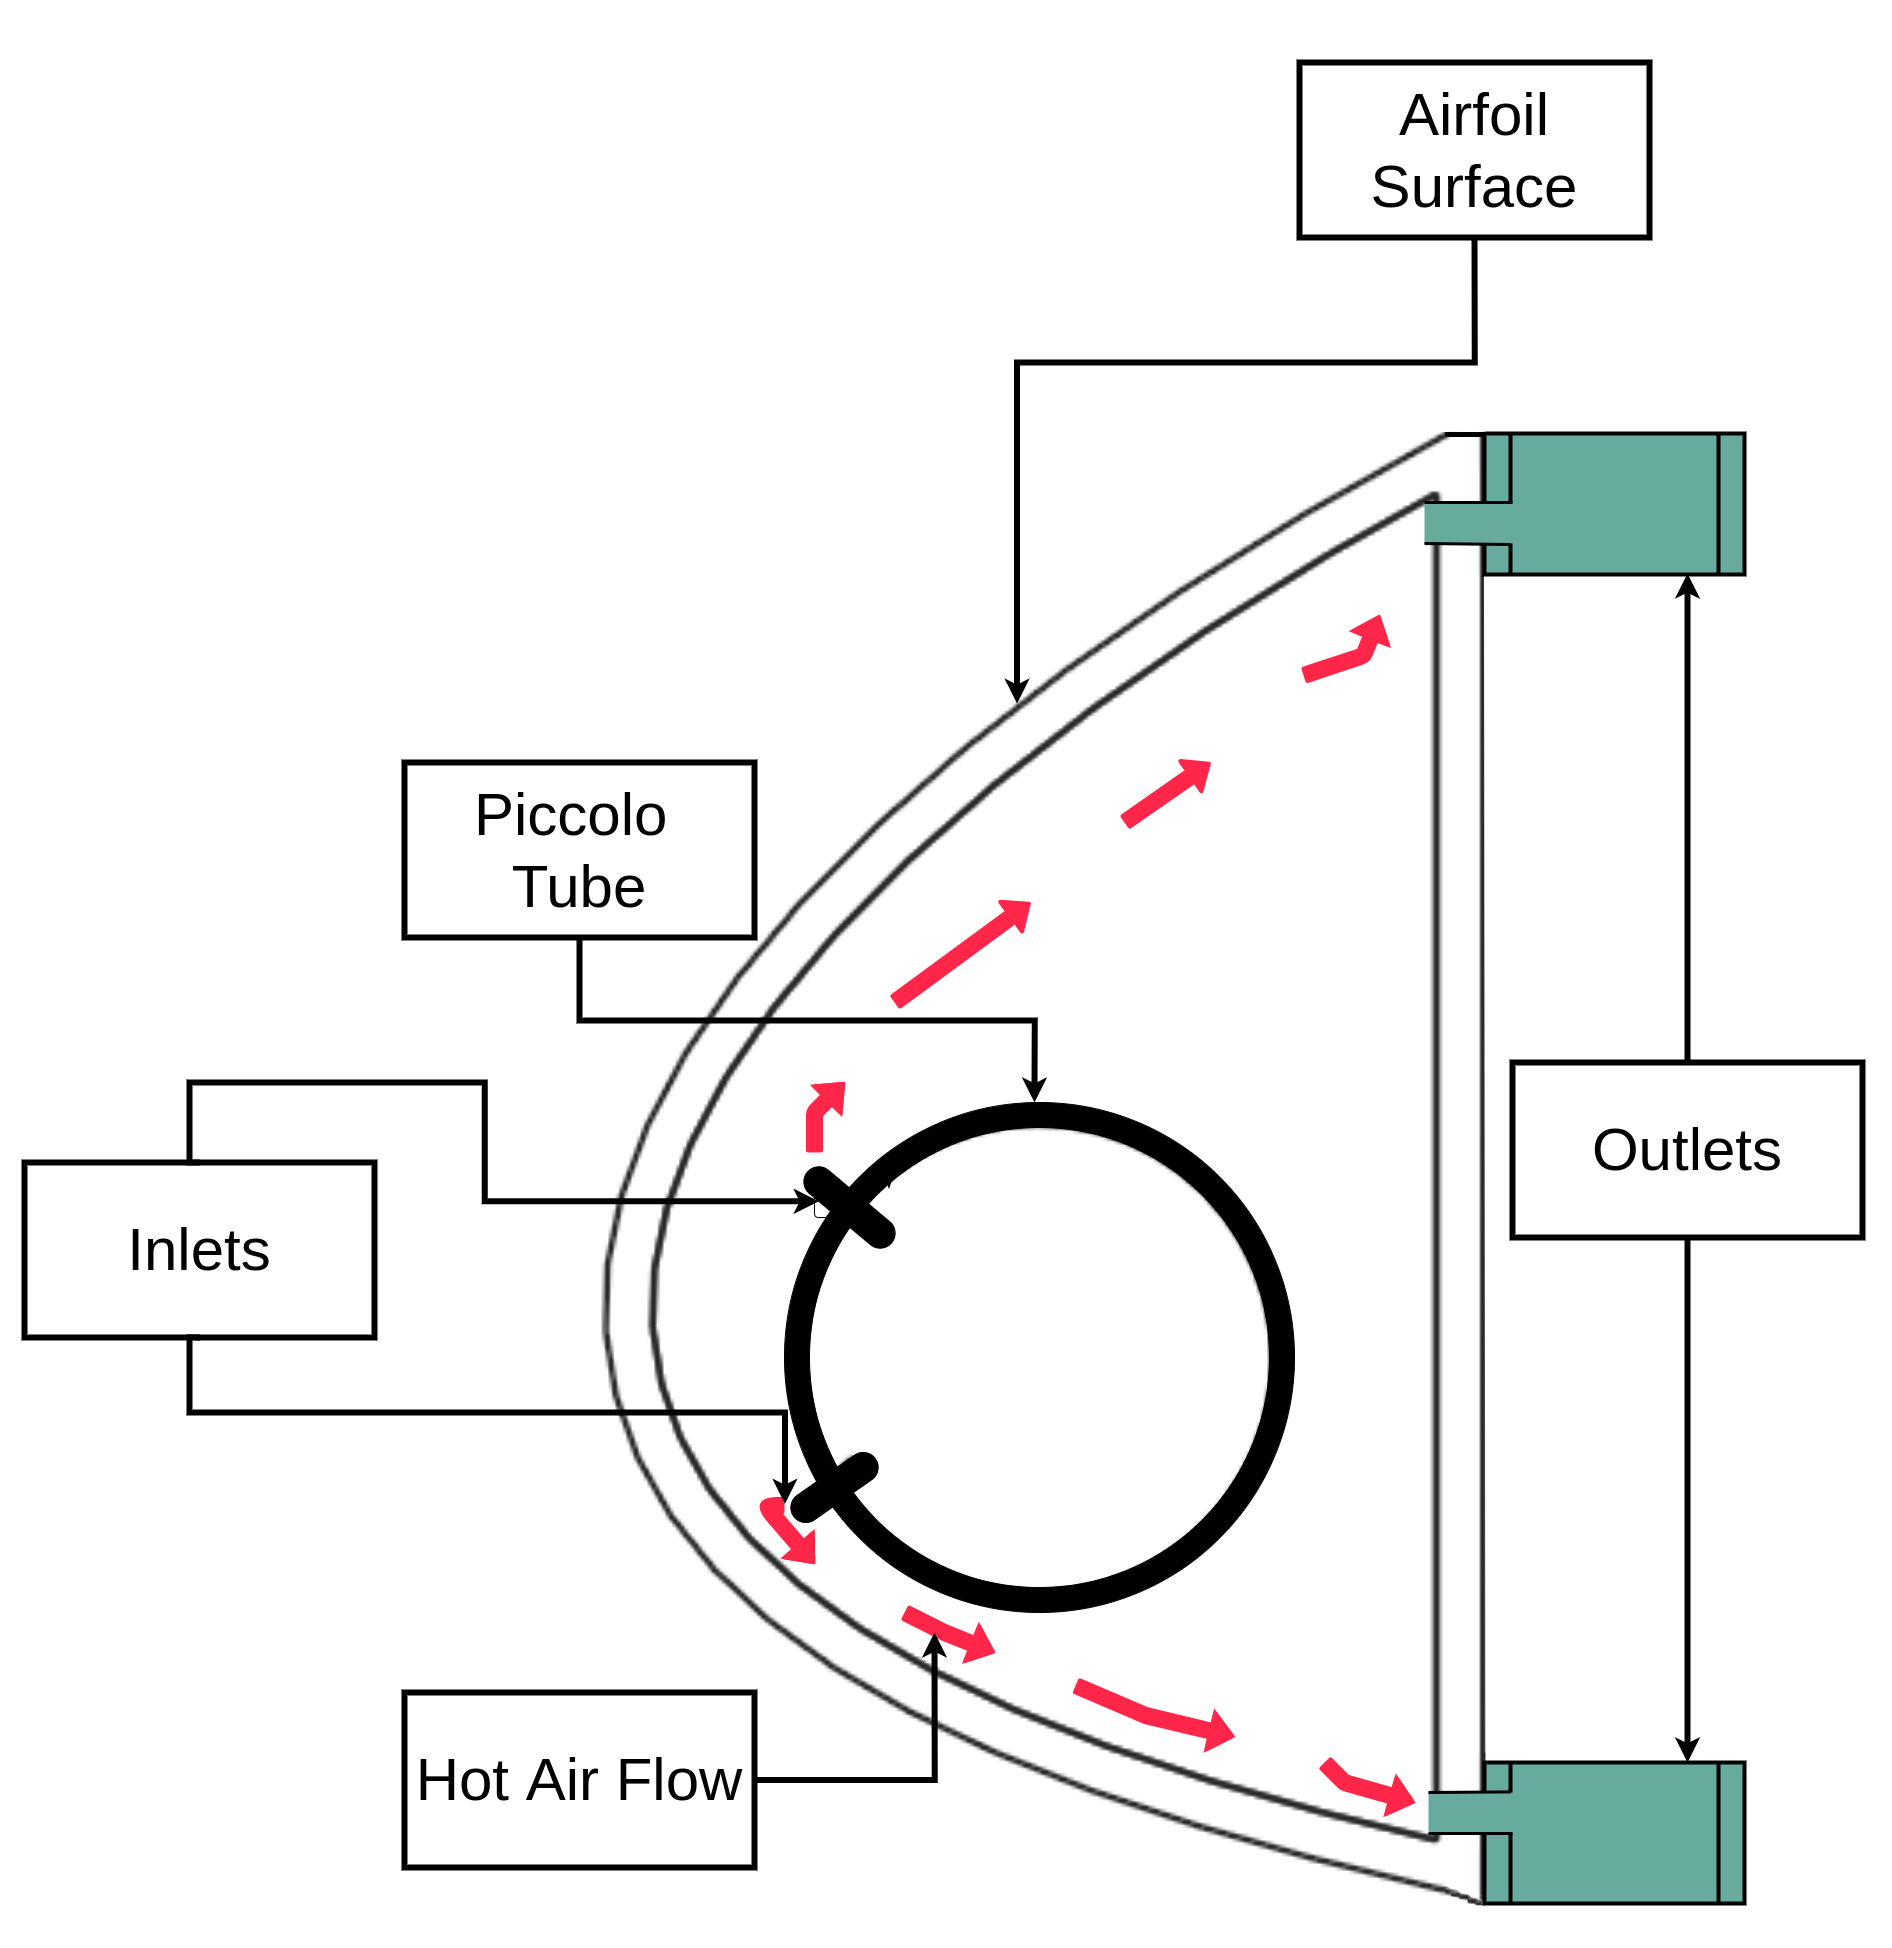
\includegraphics[width=1\textwidth,height=\textheight,scale=3.5,keepaspectratio]{Pneumatic Evaporative Anti-icing system or Piccolo Tube System.png}
\caption {Pneumatic Evaporative Anti-icing system \acrshort{wips} (\acrshort{pts})}
\label{fig:PTS}
\end{figure}


\subsubsection{Electrothermal Running-wet anti icing \acrshort{wips} (\acrshort{ets})} 
In this system, the outer airfoil surface has slabs of various materials, electric power provided heats those materials and melts the ice. The performance of (\acrshort{pts}) or \acrshort{ets} can be studied with FENSAP-ICE through the conjugate heat transfer (CHT) between air, water, ice and the solid materials that compose the \acrshort{ips}. The airflow domains are separated from the metal or composite skin of the aircraft component;, therefore, all the ANSYS airflow solvers can be used.
\todo[inline, backgroundcolor=aqua]{diagram}
For \acrshort{pts}, a steady-state thermal equilibrium between domains is computed to verify that the protected region is free of ice.
For \acrshort{ets}, the \acrshort{ips} response time to the cyclic activation of heater pads is analyzed in a time-dependent CHT simulation encompassing phase change, heat conduction and water runback to accurately predict the amount of ice that forms,
melts and refreezes. 

\subsection{Cowl Ice Protection System (CIPS)}
\label{subsec:CIPS}
\todo[inline, backgroundcolor=aqua]{equations}
\section{\acrshort{ips} Thermodynamics}
reference developments.docx
\label{sec:mathrep}
\subsection{Pneumatic Evaporative Anti-icing system \acrshort{wips}}
\subsection{Electrothermal Running-wet anti icing \acrshort{wips}}
\subsubsection{Extent of Protection (EOP)}

\section{\acrshort{ips} Weight Impact}
\label{sec:ipswtimpact}

\section{\acrshort{ips} Drag}
\label{sec:ipsdrag}
Since we have chosen the de-icing designs, there are no drag-penalties involved.

%########################################################################################
\cleardoublepage
\chapter{\acrshort{ips} Model Selection Methodology}
\label{ch:IPSparasim}
\subsection{Input Parameter Selection}
\label{subsec:inputpara}
\begin{equation}
\label{eq:barometric}
P=P_{s}\left[ 1+\frac{L_{s}}{T_{s}} \right] \left[ y-y_{s}\right]^{-g_{0}\frac{M}{R+L_{s}} }
\end{equation}
In Equation \ref{eq:barometric};  $P_s$ is the pressure at sea level or static pressure, measured in Pa. $T_s$ is the temperature at sea level or standard temperature, measured in K. $L_s$ is the standard temperature lapse rate, measured in K/m. $L_s$ has a constant value of -0.0065 K/m. The variable $y$ is the height measured about the sea level, it is measured in m. $y_s$ is the height at the bottom atmospheric layer, measured in m. $R$ is the Universal Gas Constant, which has a value of 8.31432. $g_0$ is the Gravitational Acceleration constant having a value of 9.80665 m/$s^2$. $M$ is the molar mass of the Earth's air, which has a value of 0.0289644 kg/mol \cite{presscalc}.

\subsubsection{Climb Input Parameters}
During Climb, there is a lot of power utilized to overcome drag and produce lift. When it comes to icing, the average speed taken from the flight log for our case study comes out to be 190.25 $m/s$. Icing is assumed to happen over a total duration of 500 seconds (or 8.33333 minutes). Consulting Appendix C Stratiform for droplet \acrshort{mvd} \SI{20}{\micro\metre} subject to specified air temperature and altitude, the \acrshort{lwc} is calculated. The \acrshort{lwc} is corrected for total accumulation time and cloud type to improve on the solution by introducing a correction factor. The new \acrshort{lwc} value is then used as input for the droplet simulation. Similarly, consulting Appendix C Cumuliform for droplet \acrshort{mvd} \SI{20}{\micro\metre}, the \acrshort{lwc} is calculated to be 0.255 $g/m^3$.

\begin{table}[]
\resizebox{\textwidth}{!}{%
\begin{tabular}{|l|l|l|l|l|}
\hline
Temperature at Sea Level (K)         & \multicolumn{4}{l|}{288.15}                                     \\ \hline
Pressure at Sea Level (Pa)           & \multicolumn{4}{l|}{101325}                                     \\ \hline
Altitude (ft)                        & \multicolumn{4}{l|}{6000}                                       \\ \hline
Altitude (m)                         & \multicolumn{4}{l|}{1828.8}                                     \\ \hline
Air static pressure at altitude (Pa) & \multicolumn{4}{l|}{78919.78}                                   \\ \hline
Droplet Diameter                     & \multicolumn{4}{l|}{20}                                         \\ \hline
Droplet Distribution                 & \multicolumn{4}{l|}{Langmuir D}                                 \\ \hline
Air Velocity (m/s)                   & \multicolumn{4}{l|}{80}                                         \\ \hline
Aircraft Speed (m/s)                   & \multicolumn{4}{l|}{190.25}                                         \\ \hline
Angle of Attack (degrees)                   & \multicolumn{4}{l|}{3}                                         \\ \hline
Icing air Temperature (K)            & \multicolumn{4}{l|}{256}                                        \\ \hline
Icing Duration (seconds)            & \multicolumn{4}{l|}{500}                                        \\ \hline
Clouds & \multicolumn{2}{l|}{Continuous Maximum or Stratiform} & \multicolumn{2}{l|}{Intermittent Maximum or Cumuliform} \\ \hline
Ice Type                             & \multicolumn{2}{l|}{Rime} & \multicolumn{2}{l|}{Glaze Advanced} \\ \hline
\end{tabular}%
}
\caption{Input Climb Parameters}
\label{tab:climb-table}
\end{table}

\subsubsection{Descent Input Parameters}
During Descent, there is a lot of drag induced because of application of flaps and brakes. When it comes to icing, the average speed chosen from the flight log for our case study comes out to be 202.75 $m/s$.

\begin{table}[]
\resizebox{\textwidth}{!}{%
\begin{tabular}{|l|l|l|l|l|}
\hline
Temperature at Sea Level (K)         & \multicolumn{4}{l|}{288.15}                                     \\ \hline
Pressure at Sea Level (Pa)           & \multicolumn{4}{l|}{101325}                                     \\ \hline
Altitude (ft)                        & \multicolumn{4}{l|}{6000}                                       \\ \hline
Altitude (m)                         & \multicolumn{4}{l|}{1828.8}                                     \\ \hline
Air static pressure at altitude (Pa) & \multicolumn{4}{l|}{78919.78}                                   \\ \hline
Droplet Diameter                     & \multicolumn{4}{l|}{20}                                         \\ \hline
Droplet Distribution                 & \multicolumn{4}{l|}{Langmuir D}                                 \\ \hline
Air Velocity (m/s)                   & \multicolumn{4}{l|}{80}                                         \\ \hline
Aircraft Speed (m/s)                   & \multicolumn{4}{l|}{202.75}                                         \\ \hline
Angle of Attack (degrees)                   & \multicolumn{4}{l|}{3}                                         \\ \hline
Icing air Temperature (K)            & \multicolumn{4}{l|}{256}                                        \\ \hline
Icing Duration (seconds)            & \multicolumn{4}{l|}{500}                                        \\ \hline
Clouds & \multicolumn{2}{l|}{Continuous Maximum or Stratiform} & \multicolumn{2}{l|}{Intermittent Maximum or Cumuliform} \\ \hline
Ice Type                             & \multicolumn{2}{l|}{Rime} & \multicolumn{2}{l|}{Glaze Advanced} \\ \hline
\end{tabular}%
}
\caption{Input Descent Parameters}
\label{tab:descent-table}
\end{table}

\subsubsection{Langmuir D Distribution}
Langmuir D Distribution of droplets with \acrshort{mvd} \SI{20}{\micro\metre} is used for the study. The Langmuir D distribution contains a set of seven ratios of diameters corresponding to the percentage of \acrshort{lwc}. For a given \acrshort{mvd}, there are seven values in a Langmuir D distribution. In the past, NACA has used distributions published by Langmuir to assess \acrshort{mvd} that are now in Appendix C. The upper limit for Langmuir- D distribution is an \acrshort{mvd} of \SI{50}{\micro\metre}. Figure~\ref{fig:LangmuirD} depicts the 7-diameter Langmuir-D distributions separately. The dashed line represents the final solution generated using weights on each droplet size.

\begin{figure}[!ht]
    \centering
\graphicspath{ {IPS/} }
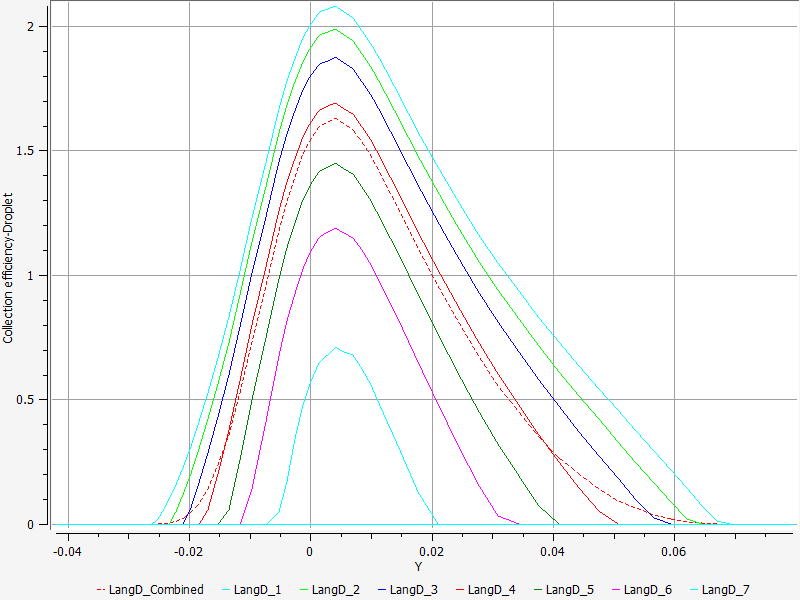
\includegraphics[width=1\textwidth,height=\textheight,keepaspectratio]{Collection_Efficiency_LangD}
\caption{Langmuir D Distribution for Climb Case Study as computed by FENSAP-ICE \cite{Habashi2004}}
\label{fig:LangmuirD}
\end{figure}

\todo[inline, backgroundcolor=aqua]{Standard NASA Parameters}
\todo[inline, backgroundcolor=aqua]{Consult page 2-F 201 of CS 25 for IPS wind tunnel testing parameters}
\todo[inline, backgroundcolor=aqua]{\acrshort{lwc} is output parameter.Flow diagram explaining the input and output parameters}


\subsection{Turbulence Model Selection}
\subsubsection{Turbulence Effects}
\label{subsec:modelsel}
The design and utilization of a mathematical model to simulate effects of turbulence constitute the initial stages of icing simulation. In most real-life scenarios, the boundary layer and wakes formed around the airplane wing are turbulent. 
Some of the observable effects of turbulent fluid flow are as follows: \cite{Davidson2018}
\begin{itemize}
  \item \textbf{Inconsistency} : Meaning that the flow is irregular in nature.
  \item \textbf{Diffusiveness} : The property refers to the extent of spreading increases as the fluid flow turns turbulent.
  \item \textbf{High Reynolds number} : Turbulence is associated with having a high Reynolds number. For a typical turbulent pipe or duct flow, the Reynolds number is more than 4000.  For the turbulent airfoils, the Reynolds number is of the magnitude of $10^6$. 
  \item \textbf{Dissipativeness}: The property refers to the tiny eddies which are formed due to turbulent flow have their own kinetic energy.
   \item \textbf{Continousness}: The property refers to the turbulence formed by the tiny eddies. The flow is treated as a continuum since the turbulence formed by the tiny eddies is much larger than the turbulence which occurs in the molecular level.
 \end{itemize}
Keeping in mind the effects observed due to turbulence, \acrshort{spt}, \acrshort{ket} and \acrshort{kost} models have been considered for \acrshort{cfd} simulations. \acrshort{cfd} has also been discussed in \ref{sec:cfd}.

\subsection{\acrfull{spt}}
\sloppy
The \acrfull{spt} is a type of one-equation \acrfull{rans} turbulence model utilized for \acrshort{cfd} simulations \cite{LangleyResearchCenter2015}. \acrshort{spt} works on computing for the solution of one partial-differential Transport equation \ref{eq:transporteq}. Equation \ref{eq:transporteq} is computed for a quantity that is derived either by the turbulent Reynolds number or turbulent Eddy Viscosity $\varpi _t$. Sutherland's Law governs the relationship between viscosity and temperature. It is assumed that the flow is compressible with Prandtl terms $Pr=0.72$ for air, and a $Pr_t=0.90$ is used for turbulent flow heat transfer.  
\begin{equation}
\label{eq:transporteq}
\begin{split}
\frac{{\partial \tilde v}}{{\partial t}} + {u_j}\frac{{\partial \tilde v}}{{\partial {x_j}}} 
& = {c_{b1}}(1 - {f_{t2}})\tilde S\tilde v - \left[ {{c_{w1}}{f_w} - \frac{{{c_{b1}}}}{{{\kappa ^2}}}{f_{t2}}} \right]{\left( {\frac{{\tilde v}}{d}} \right)^2} \\
& + \frac{1}{\sigma }\left[ {\frac{\partial }{{\partial {x_j}}}\left( {\left( {v + \tilde v} \right)\frac{{\partial \tilde v}}{{\partial {x_j}}}} \right) + {c_{b2}}\frac{{\partial \tilde v}}{{\partial {x_i}}}\frac{{\partial \tilde v}}{{\partial {x_i}}}} \right] 
\end{split}
\end{equation}
In Equation \ref{eq:transporteq}; $v$ is the Molecular kinematic viscosity and $\kappa$ is called as Von Kármán constant (logarithmic law of wall). $d$ is the distance from field point to closest wall.\\

The turbulent Eddy Viscosity $\varpi_t$ is computed by \ref{eq:eddyvis}:
\begin{equation}\label{eq:eddyvis}{\varpi _t} = \rho \tilde v{f_{v1}}\end{equation}
The variables used in \ref{eq:eddyvis} correspond to the following equations:
\begin{equation}{f_{v1}} = \frac{{{\chi ^3}}}{{{\chi ^3} + {c_{v1}}^3}}\end{equation}
\begin{equation}\chi  = \frac{{\tilde v}}{v}\end{equation}
where  $\tilde v$ refers to the viscosity-like working variable that conforms to \ref{eq:transporteq}.
\begin{equation}v = \frac{\mu }{\rho }\end{equation}
where $\rho$ represents local density and $mu$ is the dynamic molecular viscosity.
\begin{equation}\tilde S = \Lambda   + \frac{{\tilde v}}{{{\kappa ^2}{d^2}}}{f_{v2}}\end{equation}
Magnitude of Vorticity is represented by \ref{eq:magvo}
\begin{equation}\label{eq:magvo}\Lambda   = \sqrt {2{W_{ij}}{W_{ij}}} \end{equation}
\begin{equation}\label{eq:rotten}{W_{ij}} = {0.5}\left( {\frac{{\partial {u_i}}}{{\partial {x_j}}} - \frac{{\partial {u_j}}}{{\partial {x_i}}}} \right)\end{equation}
where $W_{ij}$ corresponds to the rotation tensor.
\begin{equation}{f_{v2}} = 1 - \frac{\chi }{{1 + \chi {f_{v1}}}}\end{equation}
\begin{equation}{f_w} = g{\left[ {\frac{{1 + {c_{w3}}^6}}{{g + {c_{w3}}^6}}} \right]^{1/6}}\end{equation}
\begin{equation}g = r + {c_{w2}}({r^6} - r)\end{equation}
For a large enough $r$, the variable $f_w$ becomes constant, thus maximum $r$ truncates to 10.
\begin{equation}r = \min \left[ {\frac{{\tilde v}}{{\tilde S{\kappa ^2}{d^2}}},10} \right]\end{equation}
The trip functions are represented by $f_{t1}$ and $f_{t2}$.
\begin{equation} {g_{trip}} = \min \left[ {(0.1),\frac{{\Delta U}}{{{\eta _t}\Delta x}}} \right] \end{equation}
where $\Delta x$ corresponds to wall grid spacing.
\begin{equation}{f_{t1}} = {c_1}{g_{trip}}\exp \left( { - {c_2}\frac{{{\eta _t}}}{{\Delta {U^2}}}\left[ {{d^2} + {g_{trip}}{d_{trip}}^2} \right]} \right)\end{equation}
where $d_{trip}$ corresponds to distance of field point to trip. $\Delta {U}$ is the velocity difference between field point and trip. $\eta _t$ is the wall vorticity.
\begin{equation}{f_{t2}} = {c_3}\exp ( - {c_{t4}}{\chi ^2})\end{equation}
\begin{equation}{{\tilde v}_{wall}} = 0\end{equation}
\begin{equation}3{v_\infty } \leqslant {{\tilde v}_{farfield}} \leqslant 5{v_\infty }\end{equation}

Transport equation \ref{eq:transporteq} is subject to the following free-stream boundary conditions:\\
\begin{equation}\text{Walls: \quad}{v_{t,wall}} = 0\end{equation} 
\centerline{ Outlet: Convective Outlet}
\begin{equation}\tilde S > 0\end{equation}
\begin{equation}0.210438{v_\infty } \leqslant {v_{farfield}} \leqslant 1.294234{v_\infty }\end{equation}
The values of the adjustable constants used in Transport equation \ref{eq:transporteq}:
\begin{equation}{c_{b1}} = 0.135\end{equation}
\begin{equation}{c_{b2}} = 0.622\end{equation}
\begin{equation}{c_{w1}} = \frac{{{c_{b1}}}}{{{\kappa ^2}}} + \frac{{1 + {c_{b2}}}}{\sigma }\end{equation}
\begin{equation}{c_{w2}} = 0.3\end{equation}
\begin{equation}{c_{w3}} = 2\end{equation}
\begin{equation}{c_{v1}} = 7.1\end{equation}
\begin{equation}{c_{t1}} = 1\end{equation}
\begin{equation}{c_{t2}} = 2\end{equation}
\begin{equation}{c_{t3}} = 1.2\end{equation} 
\begin{equation}{c_{t4}} = 0.5\end{equation}
\begin{equation}\sigma  = 0.666\end{equation}
\begin{equation}\kappa  = 0.41\end{equation}

Transport equation \ref{eq:transporteq} can be modified to compute for low Reynolds number \cite{LangleyResearchCenter2015}:
\begin{equation}{c_{w2,Low{R_e}}} = {c_{w4,Low{R_e}}} + \frac{{{c_{w5,Low{R_e}}}}}{{((\chi /40) + 1){)^2}}}\end{equation}
\begin{equation}{c_{w4,Low{R_e}}} = 0.21\end{equation}
\begin{equation}{c_{w5,Low{R_e}}} = 1.5\end{equation}

\subsection{\acrfull{ket}}
The \acrfull{ket} is a type of two-equation \acrfull{rans} turbulence model utilized for \acrshort{cfd} simulations. \acrshort{ket} works on computing the solution of two partial-differential Transport equations $k$-$\varepsilon$ to depict turbulence. The applications for this type of model include but are not limited to, are moderate to complex flows, flows with a high velocity gradient and viscous stresses (shear layers) and two-dimensional turbulent recirculating flows \cite{Zhang1994}.  Another version of this model is the realizable \acrshort{ket} which has a variable turbulent eddy viscosity, unlike in \ref{eq:ketturb}. It provides a better method for capturing the mean flow of complex rotational flows under high-pressure gradients and gives an improved depiction of the spreading rate. \acrshort{ket} is best suited for a flow that occurs further from the boundary.

The first transport equation depicting the turbulence kinetic energy $k$ is represented by \ref{eq:ketk} \cite{Launder1974}. ${u_i}$ represents velocity component in direction $i$.
\begin{equation}
\label{eq:ketk}
{{\delta (\rho k)} \over {\delta t}} + {{\delta (\rho k{u_i})} \over {\delta {x_i}}} = {\delta  \over {\delta {x_j}}}\left[ {{{{\varpi _t}} \over {{\sigma _k}}}} \right] + 2{\varpi_t}{S_{ij}}{S_{ij}} - \rho \varepsilon 
\end{equation}

The second transport equation depicts the dissipation $\varepsilon$. Since the explicit equation consists of unforeseen and immeasurable terms, it is amended to \ref{eq:ketdissi} \cite{Launder1974}. ${S_{ij}}$ represents the fluctuating component of rate of deformation.
\begin{equation}
\label{eq:ketdissi}
{{\delta \varepsilon } \over {\delta t}} + {{\delta (\rho \varepsilon {u_i})} \over {\delta {x_i}}} = {\delta  \over {\delta {x_j}}}\left[ {{{{\varpi_t}} \over {{\sigma _\varepsilon }}}{{\delta \varepsilon } \over {\delta {x_j}}}} \right] + {C_{1\varepsilon }}{\varepsilon  \over k}2{\varpi _t}{S_{ij}}{S_{ij}} + {C_{2\varepsilon }}\rho {{\varepsilon  \over k}^2}
\end{equation}

The Turbulent eddy viscosity $\varpi_t$ for $k-\varepsilon$ model is computed by \ref{eq:ketturb}
\begin{equation}
\label{eq:ketturb}{\varpi_t} = \rho {C_\varpi}{{k \over \varepsilon }^2}\end{equation}

\ref{eq:ketk} and \ref{eq:ketdissi} are subject to the following free-stream boundary conditions:
\begin{equation}\text{Inlet: \quad}k-\varepsilon \text{  distribution should be known. \quad}\end{equation}
\begin{equation}\text{Walls:    Solid and proportional to Reynolds number }R_e\end{equation}
\begin{equation}\text{Outlet: \quad}{{\delta \varepsilon } \over {\delta n}} = 0, \quad {{\delta k} \over {\delta n}} = 0\end{equation}

The values of the adjustable constants used in \ref{eq:ketk} and \ref{eq:ketdissi}:
\begin{equation}{C_\varpi } = 0.09\end{equation}
\begin{equation}{\sigma _k} = 1\end{equation}
\begin{equation}{\sigma _\varepsilon } = 1.3\end{equation}
\begin{equation}{C_{1\varepsilon }} = 1.44\end{equation}
\begin{equation}{C_{2\varepsilon }} = 1.92\end{equation}

\subsection{\acrfull{kost}}
Similiar to \acrshort{ket}, \acrshort{kost} is also a \acrfull{rans} two-equation model in which all the consequences of turbulence are modelled. Menter \cite{Menter1992} argues that the \acrshort{ket} model suffers from an increased prediction of the turbulence length scale in regions where the pressure gradient is not favourable, for example in the near wall region. The two transport equations account for the convection and dissipation effects concerning turbulent energy. The applications for \acrshort{kost} primarily concern low-$R_e$ flows and near-wall treatment regions. The SST refers to Shear-Stress Transport, that means that the \acrshort{kost} converts to \acrshort{ket} when the model encounters free-stream.

The first transport equation refers to the turbulence kinetic energy $k$ which is computed by  \ref{eq:kosttur}.
\begin{equation}
\label{eq:kosttur}{{\delta (\rho k)} \over {\delta t}} + {{\delta (\rho k{u_j})} \over {\delta {x_j}}} = {P_k} - {\beta ^*}\rho \omega k + {\delta  \over {\delta {x_j}}}\left[ {\left( {\varpi  + {\sigma _k}{\varpi _t}} \right){{\delta k} \over {\delta {x_j}}}} \right]\end{equation}

The second transport equation refers to the specific rate of heat dissipation that is represented by \ref{eq:kostomega}.
\begin{equation}
\label{eq:kostomega}
\begin{split}
{{\delta (\rho \omega )} \over {\delta t}} + {{\delta (\rho \omega {u_j})} \over {\delta {x_j}}} & = {\gamma  \over {{\varphi _t}}}{P_k} - \beta \rho {\omega ^2}
+ {\delta  \over {\delta {x_j}}}\left[ {\left( {\varpi  + {\sigma _\omega }{\varpi _t}} \right){{\delta \omega } \over {\delta {x_j}}}} \right] \\& + 2(1 - {F_1}){{\rho {\sigma _{{\omega ^2}}}} \over \omega }{{\delta k} \over {\delta {x_j}}}{{\delta \omega } \over {\delta {x_j}}}\end{split}\end{equation}

The Turbulent eddy viscosity $\varpi _t$ for $k-\omega$ SST model is computed by \ref{eq:turkost}.
\begin{equation}\label{eq:turkost}{\varpi _t} = {{\rho {a_1}k} \over {\max ({a_1}\omega ,S{F_2})}}\end{equation}

The variable $P_k$ represents the production term of the turbulent kinetic energy, it is computed by \ref{eq:pkkost}. There is a production limiter function applied for $P_k$.
\begin{equation}\label{eq:pkkost}{P_k} = \min \left( {{\tau _{ij}}{{\delta {u_i}} \over {\delta {x_j}}},20{\beta ^*}k\omega } \right)\end{equation}

The Turbulent shear stress $\tau _{ij}$ is computed by the relation given in \ref{eq:tau_ij}.
\begin{equation}\label{eq:tau_ij}{\tau _{ij}} = {\varpi _t}\left( {2{S_{ij}} - {0.666}{{\delta {u_k}} \over {\delta {x_k}}}\partial ij} \right) - {0.666}\rho k\partial ij\end{equation}

${S_{ij}}$ represents the fluctuating component of rate of deformation, which is computed in \ref{eq:ratedeform}.
\begin{equation}\label{eq:ratedeform}{S_{ij}} = {1 \over 2}\left( {{{\delta {u_i}} \over {\delta {x_j}}} + {{\delta {u_j}} \over {\delta {x_i}}}} \right)\end{equation}

The following equations represent the adjustable constants and auxiliary functions.
\ref{eq:blendfn} refers to the relation between the blending functions $F_1$ and $F_2$. $\Phi _1$ is the adjustable constant in the initial model and $\Phi _2$ is the adjustable constant present in the modified $k-\omega$ model.
\begin{equation}\label{eq:blendfn}\Phi  = {F_1}{\Phi _1} + (1 - {F_1}){\Phi _2}\end{equation}

The blending functions represent the adjustable constants corresponding to the $k-\varepsilon$ and $k-\omega$ models , they are computed as shown in \ref{eq:blend1} and \ref{eq:blend2}.
In \ref{eq:blend1}, $y$ is the distance to the upcoming surface.
\begin{equation}\label{eq:blend1}{F_1} = \tanh \left\{ {{{\left\{ {\min \left[ {\max \left( {{{\sqrt k } \over {{\beta ^*}\omega y}},{{500\varpi } \over {{y^2}\omega }}} \right),{{4{\sigma _{w2}}k} \over {{\xi _{k\omega }}{y^2}}}} \right]} \right\}}^4}} \right\}\end{equation}
$\xi _{k\omega }$ is the positive part of the cross-diffusion term used in \ref{eq:blend1}.
\begin{equation}{\xi _{k\omega }} = \max \left( {2\rho {\sigma _{w2}}{1 \over \omega }{{\delta k} \over {\delta {x_i}}}{{\delta \omega } \over {\delta {x_i}}}{{,10}^{ - 10}}} \right)\end{equation}
\begin{equation}\label{eq:blend2}{F_2} = \tanh \left[ {{{\left[ {\max \left( {{{2\sqrt k } \over {{\beta ^*}\omega y}},{{500\varpi } \over {{y^2}\omega }}} \right)} \right]}^2}} \right]\end{equation}
Other auxilliary relations between the variables are \ref{eq:magvo} for the magnitude of vorticity $\Lambda$, and a rotation tensor ${{W_{ij}}}$ which follows the same relation as previously mentioned in \ref{eq:rotten}.

\ref{eq:kosttur} and \ref{eq:kostomega} are subject to the following boundary conditions in the \acrshort{kost} model.

\begin{equation}{k_{wall}} = 0\end{equation} 
\begin{equation}{{w_{wall}} = 10{{6\varpi } \over {{\beta _1}{{(\Delta {d_1})}^2}}}}\end{equation} 
\begin{equation}\label{eq:rel}{{{U_\infty }^2} \over {\psi}} < {\omega _{farfield}} < 10{{{U_\infty }} \over \psi}\end{equation}
In \ref{eq:rel}, the term $\psi$ is the length estimate of the computational domain.
\begin{equation}{{{{10}^{ - 5}}{U_\infty }^2} \over {{R_{e\psi }}}} < {k_{farfield}} < {{{U_\infty }^2} \over {10\psi }}\end{equation}

Auxiliary adjustable constants are:
\begin{equation}{\gamma _1} = {{{\beta _1}} \over {{\beta ^*}}} - {{{\sigma _{w1}}{\kappa ^2}} \over {\sqrt {{\beta ^ + }} }}\end{equation}

\begin{equation}{\gamma _2} = {{{\beta _2}} \over {{\beta ^*}}} - {{{\sigma _{w2}}{\kappa ^2}} \over {\sqrt {{\beta ^ + }} }}\end{equation}

\begin{equation}{\sigma _{w1}} = 0.5 \end{equation}
\begin{equation}{\sigma _{w2}} = 0.856  \end{equation}
\begin{equation}{\sigma _{k1}} = 0.85 \end{equation}
\begin{equation}{\sigma _{k2}} = 1 \end{equation}
\begin{equation}{\beta _1} = 0.075 \end{equation}
\begin{equation}{\beta _2} = 0.0828 \end{equation}
\begin{equation}{\beta ^*} = 0.09 \end{equation}

\subsection{Rationale for model selection}
It has been observed from a large number of experiments that the Spalart-Allmaras solutions converge much faster and simpler than the $k-\omega$ SST model since only one computation of the transport equation is performed in \acrshort{spt}. Values for adjustable constants used in all of the three models are produced after data-fitting an extensive range of free turbulent flows. \acrshort{ket} is not suitable for near-wall treakment. Due to the implementation of Shear Stress transport equation, \acrshort{kost} provides better implementation and prediction of complex flow separation and enhanced near-wall treatment. Another significant advantage is its high precision to cost ratio. Additionally, \acrshort{kost} offers highly accurate velocity profiles. \acrshort{kost} is the most popular model in the industry, and all of the reasons provide significant confidence to select \acrshort{kost} as our go-to model for all simulations . 
\todo[inline, backgroundcolor=aqua]{review it again}
%########################################################################################
\cleardoublepage
\chapter{\acrshort{ips} Software Selection Methodology}
\label{ch:IPSsoft}
\subsubsection{Introduction}
The practical procedure to address the scientific problems faced in the study are done by simulations and four different programming languages, namely MATLAB, Fortran (XFoil), C++ (XFoil, Gmsh) or at times, Python-based languages (Gmsh geo, Ironpython). The chapter discusses in detail the alternatives available. The latter part of the chapter illustrates the stages involved in the simulation approach.

\subsection{\acrfull{cfd}}
\label{sec:cfd}
\acrshort{cfd} is an effective fluid dynamics tool. Fluid flows and associated theories that Differential Equations can describe can sometimes be analytically complicated to compute. The models presented in the previous chapter \ref{subsec:modelsel} help to propose a method of discretization that approximates equations by an algebraic equation system. Some of the software packages discussed in this chapter are \acrshort{cfd} packages.

\subsection{Software Package Selection}
\label{subsec:softpaksel}
This section attempts to provide a brief description of the software alternatives and catalogues the challenges encountered when selecting a specific package.
\subsubsection {\acrshort{openfoam}-Paraview}
\acrshort{openfoam} is an open-source \acrshort{cfd} package which requires prior working knowledge of Python. The package has a six-month release cycle, making it increasingly efficient for support of new hardware. A major limitation is that it requires a sophisticated installation (docker based binaries for a non-unix system). \textbf{The standard libraries that are available in \acrshort{openfoam} do not support icing implementations}. Furthermore, since the package is a command-line interface (CLI) program, it requires an additional post-processing package called ParaView for viewing data analysis and visualization graphics. Essentially, \acrshort{openfoam} is more of a library for creation of executable scripts, than a generic software package. Figures \ref{fig:openfoam} and \ref{fig:paraview} portray the cavity tutorial running on a Unix system.
\begin{figure}[!ht]
    \centering
    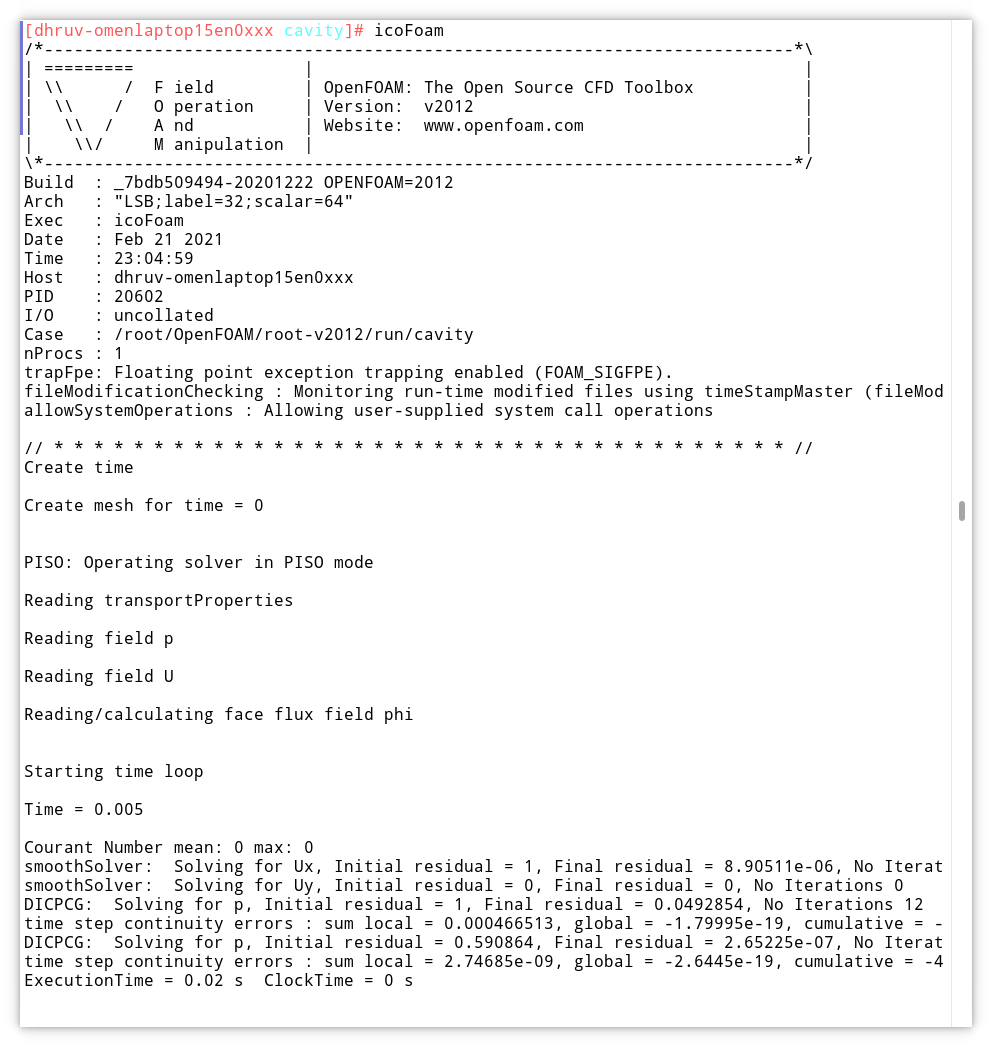
\includegraphics[width=0.8\textwidth]{IPS/openfoam.png}
    \caption{\acrshort{openfoam} Cavity tutorial running on Unix.}
    \label{fig:openfoam}
\end{figure}
\begin{figure}[!htb]
    \centering
    \includegraphics[width=1\textwidth]{IPS/paraview.png}
    \caption{Paraview Cavity mesh generation on Unix.}
    \label{fig:paraview}
\end{figure}

\subsubsection {MATLAB Simulink \textsuperscript{\textregistered}}
Skinkafi and Lawson \cite{shinlaw1} proposed a MATLAB Simulink \cite{simulink} model to calculate the IPS loads and implement the icing system. Their model consists of 12 inputs for studying aircraft, atmospheric conditions, and implementation of mission-related parameters. The primary application of this type of model is that it is used for the optimisation of flight trajectory, and not merely the implementation of the IPS. Since the objective is outside the scope of this study, this method was not implemented. However, the data and the verification results provided in \cite{shinlaw1} give a comprehensive evaluation of the integration of the IPS with the other systems as a whole. The reasons presented make it an excellent alternative to the solution provided in this thesis. \ref{fig:simulink} provides an example of a Simulink model.
\begin{figure}[!htb]
    \centering
    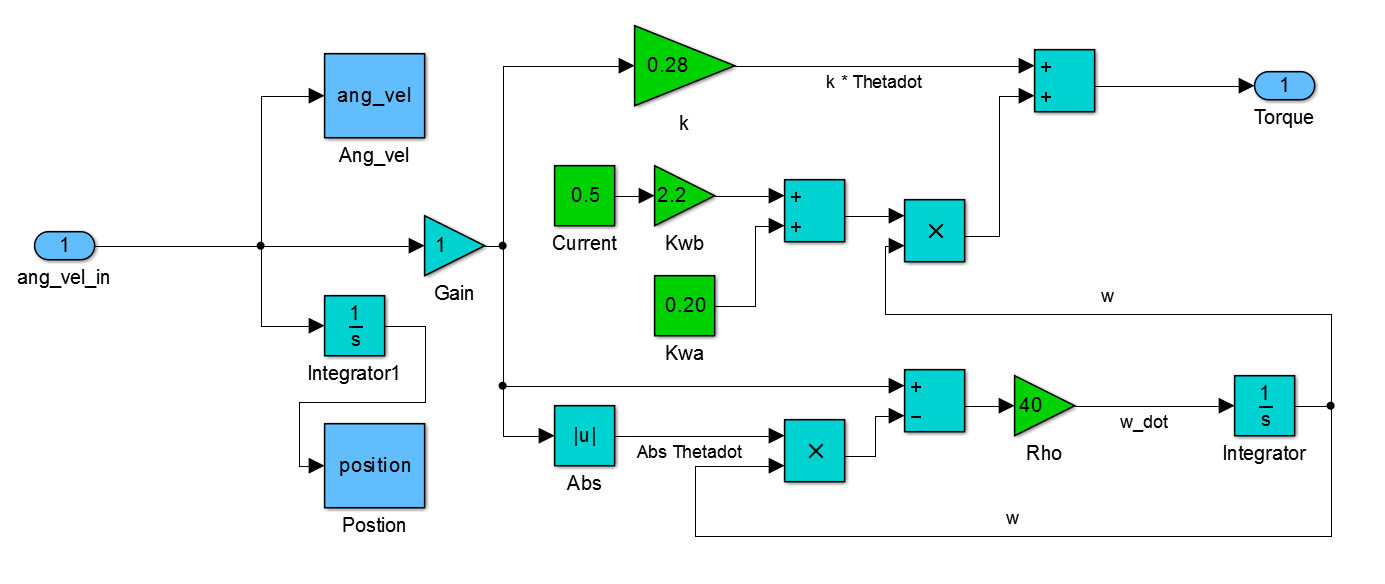
\includegraphics[width=1\textwidth]{IPS/Bilde_av_Dahl_model.png}
    \caption{Simulink example of Dahl Friction model.}
    \label{fig:simulink}
\end{figure}
\subsubsection {Gmsh}
\label{subsubsec:gmsh}
Gmsh is a 3D, open-source CAD-based software package. It generates a finite element mesh. The user interface of Gmsh provides a lightweight and simple tool while providing parametric scripting input options. The input parameters can be scripted as Gmsh supports programming languages such as Gmsh geo, Python and Julia. The Gmsh interface uses OpenCascade engine for geometry generation. The mesh libraries are based on Mmg3d and Netgen. The input geometry files can either be scripted using the Gmsh geo Programming language, or \lstinline{.STEP} files. The output mesh formats are \lstinline{.msh}, Nastran Bulk Data file \lstinline{.bdf} and STL Surface \lstinline{.stl} files. In addition, Gmsh supports post-processing and generates the file \lstinline{.pos} format. A major advantage of Gmsh is that it utilizes the GNU General Public License v2, which makes code and file sharing easier \cite{gmsh}.\\
\textbf{Side Note}: The initial approach to mesh generation involved the use of Gmsh as shown in  \ref{fig:icingsim}, and the code was developed for it. However, the \textbf{mesh file generated using Gmsh could not be used inside ANSYS because ANSYS is proprietary software}. Error log for the same is represented in \ref{fig:ansys_error_gmsh}. Thus, the method of developing further code for Gmsh was dropped. Consequentially, the mesh generated using ANSYS Meshing could also not be read by Gmsh, as shown in \ref{fig:gmsh_error_ansys}. Considerable amount of time and resources were spent trying to develop code that is consistent with the case study provided in the thesis. Since the generated mesh was open-source, and the package provides simple scripting for automation, the code is included for this study. Alternatives may be further developed in the future. The scripting options are presented in as part of the MATLAB Code \ref{dhruvmatlabcode}. The code automatically downloads the required Gmsh program files from the dhruvhaldar Github repository, and generates a mesh by automatically running Gmsh based on the variables defined in \ref{dhruvmatlabcode}. Sections \ref{subsec:gmsh_geometry}  and \ref{subsec:gmsh_mesh} discuss in detail how the geo programming language is used inside \ref{dhruvmatlabcode} to generate a mesh.
\begin{figure}[!htb]
    \centering
    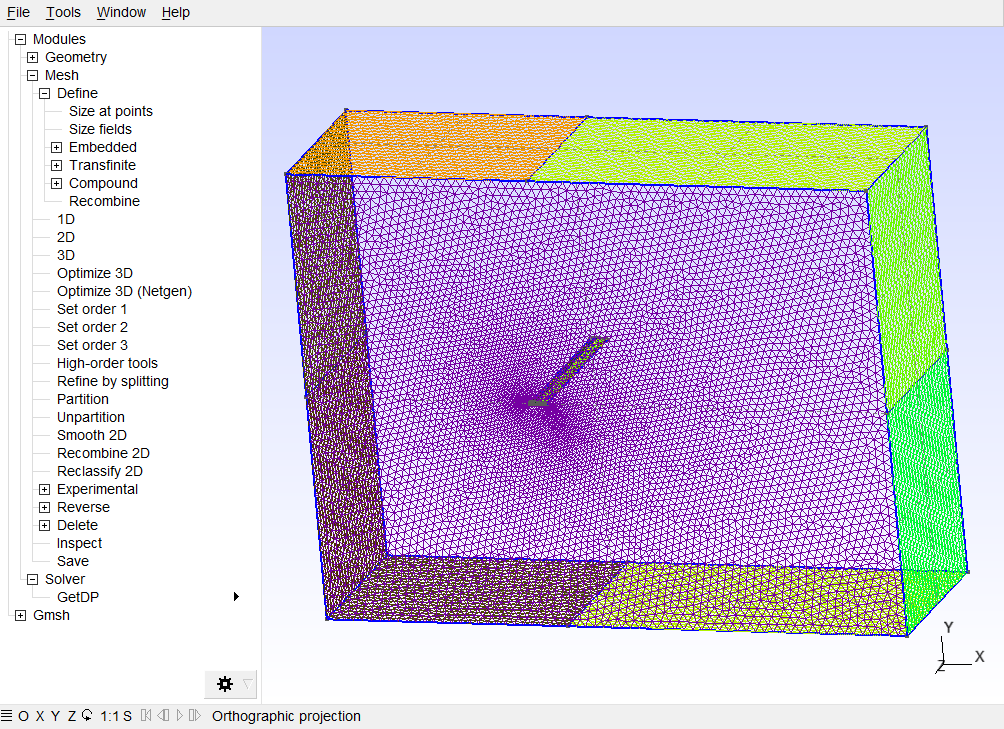
\includegraphics[width=1\textwidth]{IPS/gmsh.png}
    \caption{Automated Mesh Generated in Gmsh using \ref{dhruvmatlabcode}.}
    \label{fig:gmsh}
\end{figure}
\subsubsection {FreeCAD}
A python-based macro available for FreeCAD was used to read the airfoil coordinate files \cite{freecad}. The geometry created in the process was then exported to Gmsh. However, with the implementation of Gmsh Automation and Scripting this additional FreeCAD software dependency was removed, this is graphically represented in \ref{fig:icingsim}.
\subsubsection {ANSYS FLUENT}
The package has been used for implementation of \acrshort{pts} and \acrshort{ets} \acrshort{ips} systems.
\subsubsection {ANSYS FLUENT Icing}
FLUENT Icing is a simpler version of FENSAP-ICE \cite{Habashi2004} mainly used to compute generic airflow problems related to icing. The package supports basic atmospheric parameters and droplet distribution, and requires that the case files be computed from FLUENT. Thus, there is no option to create or modify a file from scratch. It supports input of basic input atmospheric conditions and droplet distribution. The major limitation of this package is that there is not enough documentation available \cite{fluenticing}.
\subsubsection {ANSYS FENSAP-ICE}
Cite \cite{Habashi2004}
\todo[inline, backgroundcolor=aqua]{Insert picture}
\subsubsection {ANSYS SpaceClaim}
Cite \cite{spaceclaim}.Section \ref{subsec:ironpython_geometry} discusses in detail how IronPython \ref{dhruvironpythoncode} was utilized inside the SpaceClaim interface to generated airfoil geometry for ANSYS.
\todo[inline, backgroundcolor=aqua]{Insert picture}
\subsubsection {XFoil}
\begin{figure}[!htb]
    \centering
    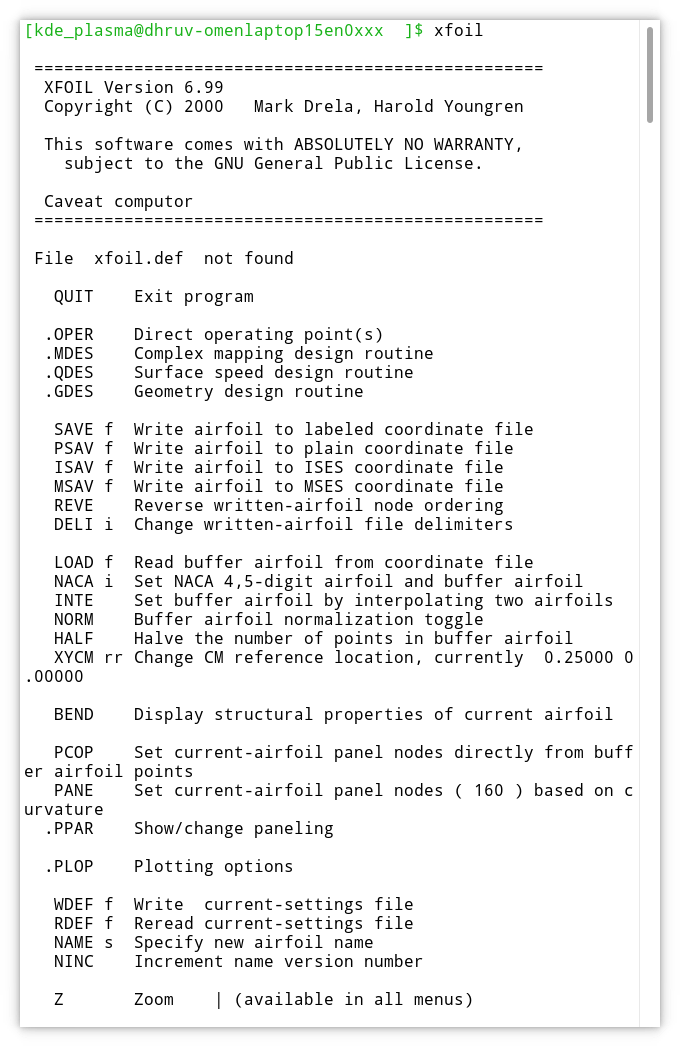
\includegraphics[width=0.8\textwidth]{IPS/xfoil1.png}
    \caption{XFoil running on Unix\textsuperscript{\textregistered}.}
    \label{fig:xfoil1}
\end{figure}
Figure reference \ref{fig:xfoil1}
XFoil cite \cite{xfoil}\\Section \ref{subsec:airfoil_geometry} gives an in-depth analysis of how \ref{dhruvmatlabcode} was exploited XFoil to generate the airfoil coordinate data file.
\todo[inline, backgroundcolor=aqua]{Insert picture}
\subsubsection {AirfoilTools.com Website} 
The website \cite{airfoiltools} is not a software per-se, however it is worth mentioning that the website provides detailed modification options for generating an airfoil. The underlying engine utilizes XFoil engine and Airfoil database from University of Illnois website \cite{uiuc}.

\subsection{Rationale for software selection} It is essential that students and researchers should be able to repeat the conditions described in this study to get the same results. The ANSYS SpaceClaim and ANSYS FENSAP-ICE software package available is bleeding-edge. However, both help us to attain the objective within respectable assumptions. Additionally, ANSYS FENSAP-ICE is the only software that has an extensive set of features necessary for IPS.

\todo[inline, backgroundcolor=aqua]{openness, limitations, advantages, latest}

\subsection{System specifications and Program runtime} 
The softwares was run on a 64-bit processor architecture with 16 GB of RAM. Since, the Fluent simulations normally take a longer amount of time, they were run on a separate 6-core 64-bit processor running on 32 GB RAM. The initial approach took about 20 minutes from start to finish. The newer approach, however, in which the geometry and mesh generation were modified and optimized, reduced the program runtime to approximately 3 minutes. A similar approach to optimizing the MATLAB code \ref{dhruvmatlabcode} was implemented, the \lstinline{if-else} statements present in program code were changed to \lstinline{while} loops significantly reducing the execution speed. This actively demonstrates that the compiler will only run that particular line of code if the \lstinline{while} loop argument is true. Additionally, an option for multi-platform support has also been included in \ref{dhruvmatlabcode} as evident by the \lstinline{ispc} function.
%########################################################################################
\cleardoublepage
\chapter{Icing Simulation}
This chapter discusses in detail each of the elements used to create the flowchart \ref{fig:icingsim}. \ref{fig:icingsim} shows how the different software packages and files are connected together in an iterative form. It also shows the failed and abandoned approaches used to arrive at the solution. The orange parallelograms used in \ref{fig:icingsim} refer to the input and output files generated during the process. The green rectangles in \ref{fig:icingsim} represent the process, or software packages used, The purple box in \ref{fig:icingsim} represent the sub-process occurring within the process, where additional input parameters are given during each step of the iterative simulation.
\begin{figure}[!htb]
    \centering
    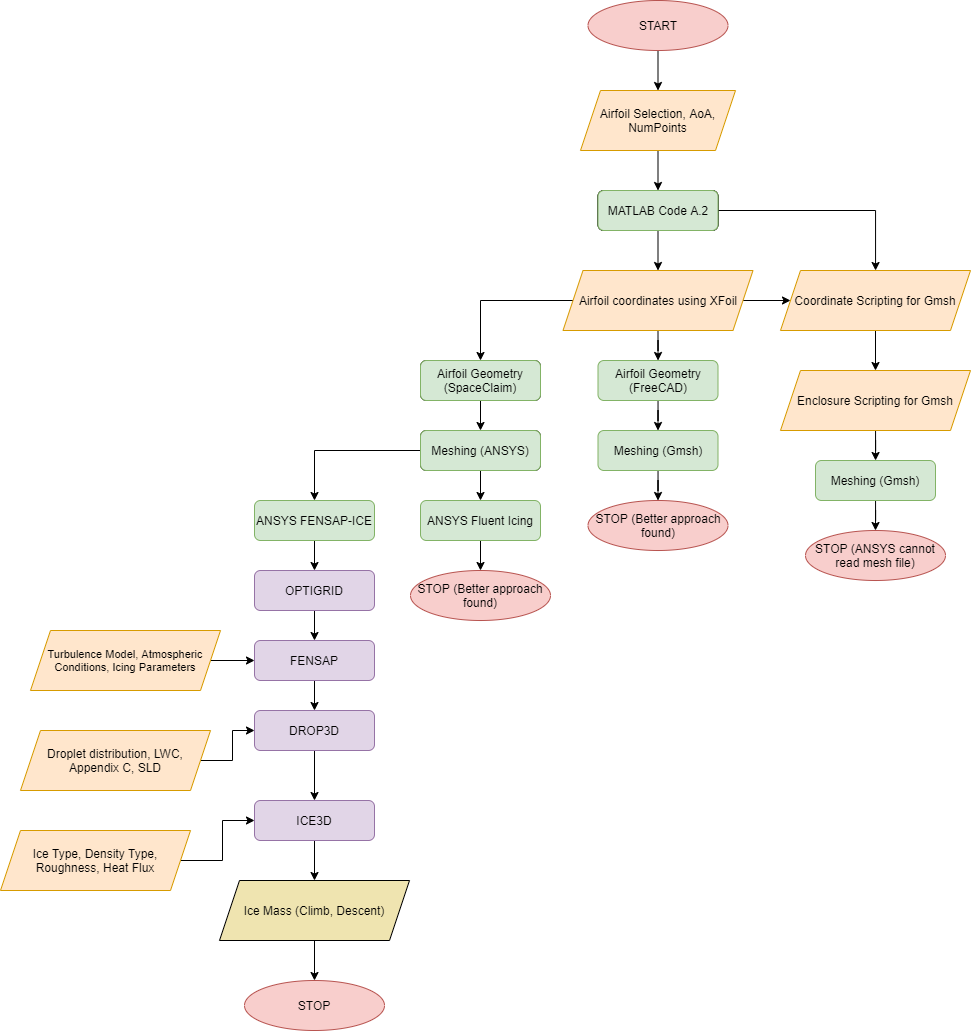
\includegraphics[width=1\textwidth]{IPS/Icing Simulation.png}
    \caption{Flowchart of Icing Parameters Simulation.}
    \label{fig:icingsim}
\end{figure}
\subsection{Airfoil Geometry} \label{subsec:airfoil_geometry}
Figure \ref{fig:xfoil2} shows the plot of the coordinate file generated by XFoil.
The airfoil file is generated from \ref{dhruvmatlabcode} which exploits XFoil for the points generation. A modified version NACA 24012 with closed trailing edge is the airfoil selected for this case study. 
\begin{figure}[!htb]
    \centering
    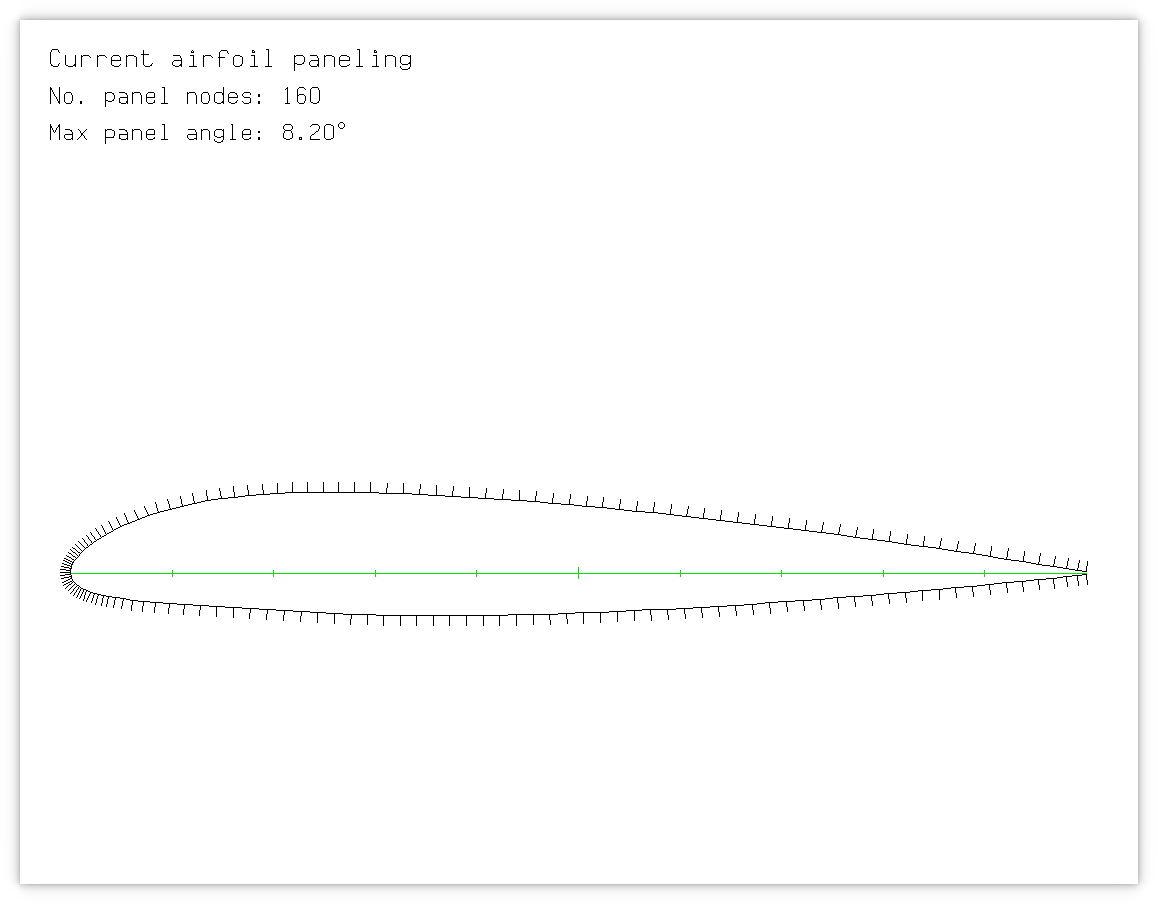
\includegraphics[width=0.8\textwidth]{IPS/xfoil2.png}
    \caption{NACA 24012 Airfoil Geometry generated using XFoil.}
    \label{fig:xfoil2}
\end{figure}
xfoil cite\cite{xfoil}
gmsh cite\cite{gmsh}
FreeCAD cite
\subsection{ANSYS Meshing}
Very time consuming since orthogonal quality is difficult to achieve in 3D meshing.A compromise between 1.5 million mesh elements and defeaturing is the objective.
\subsection{Meshing Y+ Value}
\subsection{Gmsh Geometry Automation} \label{subsec:gmsh_geometry}
MATLAB Code
\subsection{IronPython Geometry Automation} \label{subsec:ironpython_geometry}
The default airfoil coordinate file that was generated from XFoil consists of two columns relating to the x and y coordinates. In order to make the file compatible with IronPython, a modified airfoil file consisting of placeholders and curve name was generated. A new command was added to the first line of the script \lstinline{Polyline=True}. The \lstinline{Polyline} command created a 2D spline curve out of the data points (Airfoil Coordinates). For the \lstinline{Polyline} command to work, the first column in the data points (Airfoil Coordinates) shall have integer values. Thus, the first column consisted of the curve number (1 in our case). This is represented in Figure \ref{fig:airscript}. Additionally, the coordinates were scaled by 1000 since the SpaceClaim user interface by default has mm as the set unit of length. \hfill \break
The modified script was then imported into the IronPython script as a part file. There are two ways for running the script. First is in debug mode, where the compiler runs the script line-by-line. Second, the program runs the entire script all at once. These two options are important to differentiate since the IronPython compiler is bleeding-edge, sometimes one worked better over the other. \lstinline{Fit=True} could also be added to Curve fit the coordinate points within a specified tolerance \lstinline{Fittol}.
\begin{figure}[!htb]
    \centering
    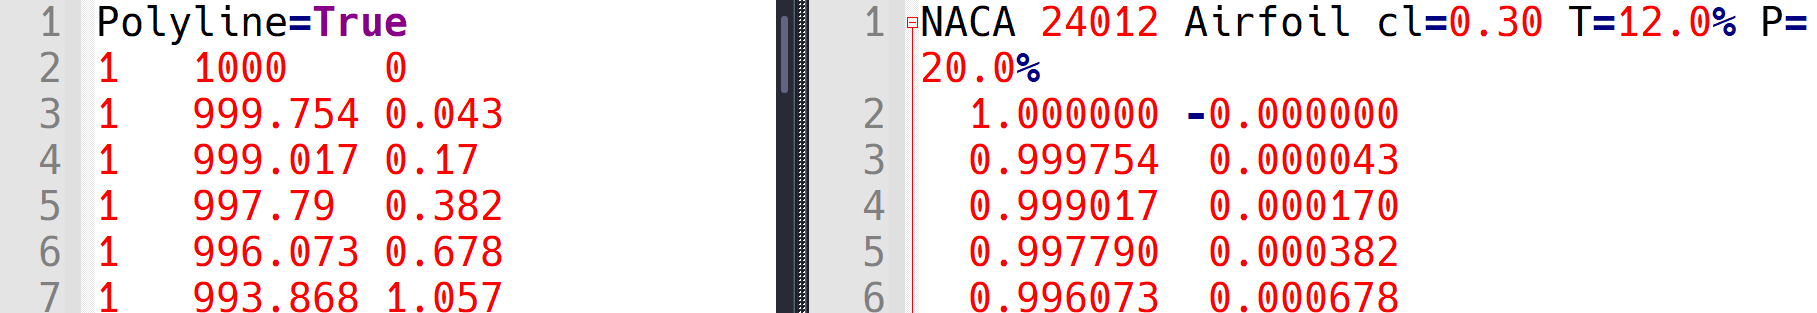
\includegraphics[width=1\textwidth]{IPS/notepad++_woSEXWc0kh.png}
    \caption{Modified Script vs Original NACA 24012 Airfoil.}
    \label{fig:airscript}
\end{figure}

\subsection{Gmsh Meshing} \ref{dhruvmatlabcode} Unfortunately, Gmsh file couldn't be used in the ANSYS model.
\subsection{Gmsh Meshing Automation} \label{subsec:gmsh_mesh}
\subsubsection{Gmsh Enclosure Automation}
\subsubsection{Gmsh Surface Automation}
\subsection{ANSYS SpaceClaim Mesh Scripting Automation}
By default, the IronPython SpaceClaim scripting works only for geometry creation. Yet, there was an option to enable meshing automation inside SpaceClaim itself. The meshing method had very limited and basic features, as it was meant for simpler objects (geometries). The command \lstinline{SetFaceMeshTypeOptions()} was used to enable meshing and set the meshing options supported in the ANSYS Meshing software (separate software package inside ANSYS). The \lstinline{SetFaceMeshTypeOptions()} command seemed to work in the initial iteration of geometries made. However since the SpaceClaim mesh compiler was bleeding-edge, the compiler kept on crashing. This became more prevalent as the newer iterations made the airfoil geometry more complicated. Hence, the utilization of SpaceClaim scripting for meshing automation was dropped. However, the compiler should work fine as the product gets developed in further releases of the ANSYS Software package. An example of a meshing block which was used in the initial iterations for geometry creation is included in . 

\subsection{Mesh Optimization} Mesh size, orthogonal quality, $y+$ value, OPTIGRID

\subsection{IPS Implementation and Calculation}
Discussion of FENSAP-ICE, DROP3D, ICE3D, CHT3D Pneumatic, CHT3D Electrothermal.

\todo[inline]{paraphrase the following text}
The physics and in-flight icing thermodynamics consist of strong heat convection in fluids. Realistic simulations of IPS are too complex to be treated within a single computational domain. The computationally efficient alternative is to apply a divide and conquer strategy by computing the solutions of the different domains separately and exchanging interface boundary conditions in an iterative manner. Convergence is achieved by equalizing heat fluxes and temperatures across interfaces. The strategy also benefits from simplification of mesh modeling.
%########################################################################################
\cleardoublepage
\chapter{Bleed Temperature}
\label{ch:bleedtemp}
%\todo[inline, backgroundcolor=aqua]{Short description why bleed temperature is important.}
This chapter will show the relationship between bleed-air temperature and net thrust for the CFM56-5B turbofan engine. Fuel consumption due to bleed-air extraction from the engines is a function of bleed temperature. Though many different machines fly today, each with its characteristics, to limit the amount of work, the engine that the A320 family widely uses was chosen for the model. It will be a source of error when comparing the calculations with aircraft that runs with other engines. Still, the differences should be limited because the engine manufacturers are assumed to be working with similar physical limits and goals.

\section{CFM International CFM56-5B}
\label{sec:cfm56-5b}
%\todo[inline, backgroundcolor=aqua]{Describe the CFM56-5B roughly. Show bleed ports.}
The CFM56-5B is a high bypass ratio turbofan engine with two concentric spools. The low-pressure parts (fan, LPC and LPT) are connected to the inner spool, while the high-pressure parts (HPC and HPT) are attached to the outer spool. Bleed air is extracted for internal use, in the engine, and external use by the aircraft pneumatics. Depending on pressure requirements, bleed air can be tapped from several different locations. For the aircraft, bleed-air can be taken downstream right after the LPC and after the 5th stage of the HPC.

\subsection{Engine Maps}
\label{subsec:enginemaps}
%\todo[inline, backgroundcolor=aqua]{Engine maps. Show how bleed temperature is a function of thrust.}
%\todo[inline, backgroundcolor=aqua]{Include picture.}
A way to describe the characteristics of a turbojet engine is to use compressor maps and turbine maps. Since we are only interested in bleed temperature from the compressor stages, we will only use compressor maps. Relevant maps for the CFM56-5B can be seen in figure \ref{fig:CFM56-5BMaps}.
%\todo[inline, backgroundcolor=aqua]{Show maps for Fan, LPC and HPC. With extrapolated operation points.}

\begin{figure}[hb]
    \centering
    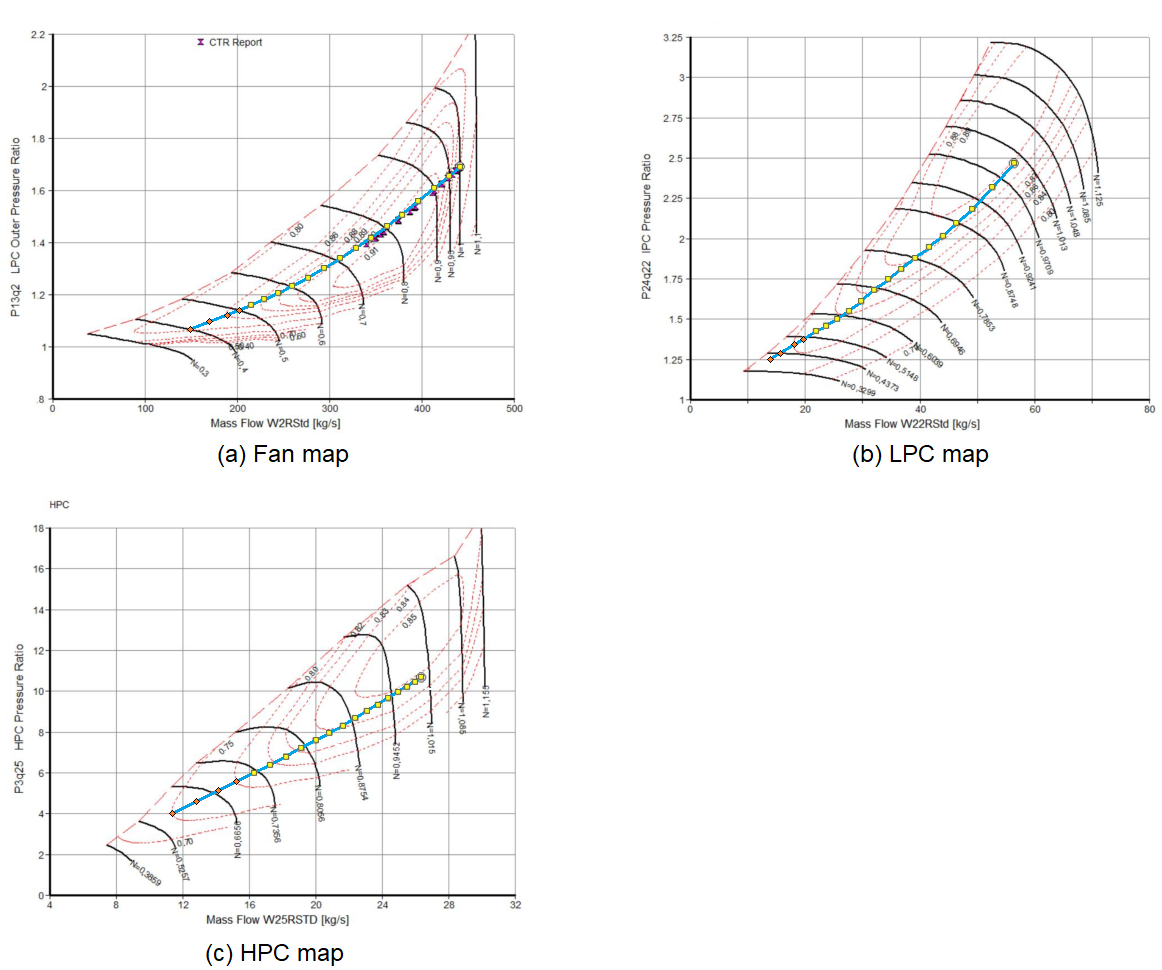
\includegraphics[width=1\textwidth]{Epictures/CFM56-5B_Compressor Maps.png}
    \caption{CFM56-5B maps with extrapolated orange points. Amended from Baptista, 2017, \cite{Baptista2017}.}
    \label{fig:CFM56-5BMaps}
\end{figure}

These maps show, for standard sea-level condition, the relation between air mass flow rate through the engine, the pressure ratios, the rotational speeds, efficiency and most importantly, the operation of the engine.
%The engine controller will strive to maximize the overall efficiency of the engine, by keeping the operation point in each map in a high efficiency region.

Ideally, maps from the engine manufacturer should be used, but they are not publicly available. Maps presented here are based on standard maps by various sources, compiled by the \textit{GasTurb} company, \cite{Kurzke2020}.
% See figure \ref{fig:GasTurbCompMapSource} and \ref{fig:GasTurbTurbMapSource}

The yellow squares in the maps show different operation points of the engine. The point with the highest mass flow rate corresponds to the engine's maximum thrust condition, as the mass flow rate is proportional to thrust. All the points are placed on operation lines.

\textit{GasTurb} provides tools to adjust generic maps to fit a specific engine. This has been done by Baptista, 2017, \cite{Baptista2017}, to obtain the maps presented in figure \ref{fig:CFM56-5BMaps}. Extrapolated points were added as orange diamonds to the maps to lower the engine's operation limit, enabling a lower idling setting for the simulations. Care has been taken to keep some surge margin.

What dictates the shape and placement of the operation lines? It is assumed that the engine's controller strives to maximize the overall efficiency by placing the operation points in high-efficiency areas while balancing the power between compressors, turbines, power off-takes, bleed air, and fuel injection.
Safety limits, such as surge margin and spool speed, must also be considered by the controller. The shape and placement of the operation lines are then assumed to be decided by the controller.

Example of how different loads on a generic engine changes the operation lines are shown in figure \ref{fig:GasTurbHPCMapBleed} and \ref{fig:GasTurbHPCMapPower}. Increased bleed-air flow rate moves the operation line further down to the right, away from the surge line. Increased mechanical power off-take moves the operation line closer to the surge line. This behaviour shows that engines for More Electric Aircraft, with large mechanical power extraction, must be designed for the specific purpose to keep the same surge margin.
To limit the amount of work, operation lines are kept static according to figure \ref{fig:CFM56-5BMaps}.

\begin{figure}[hb]
    \centering
    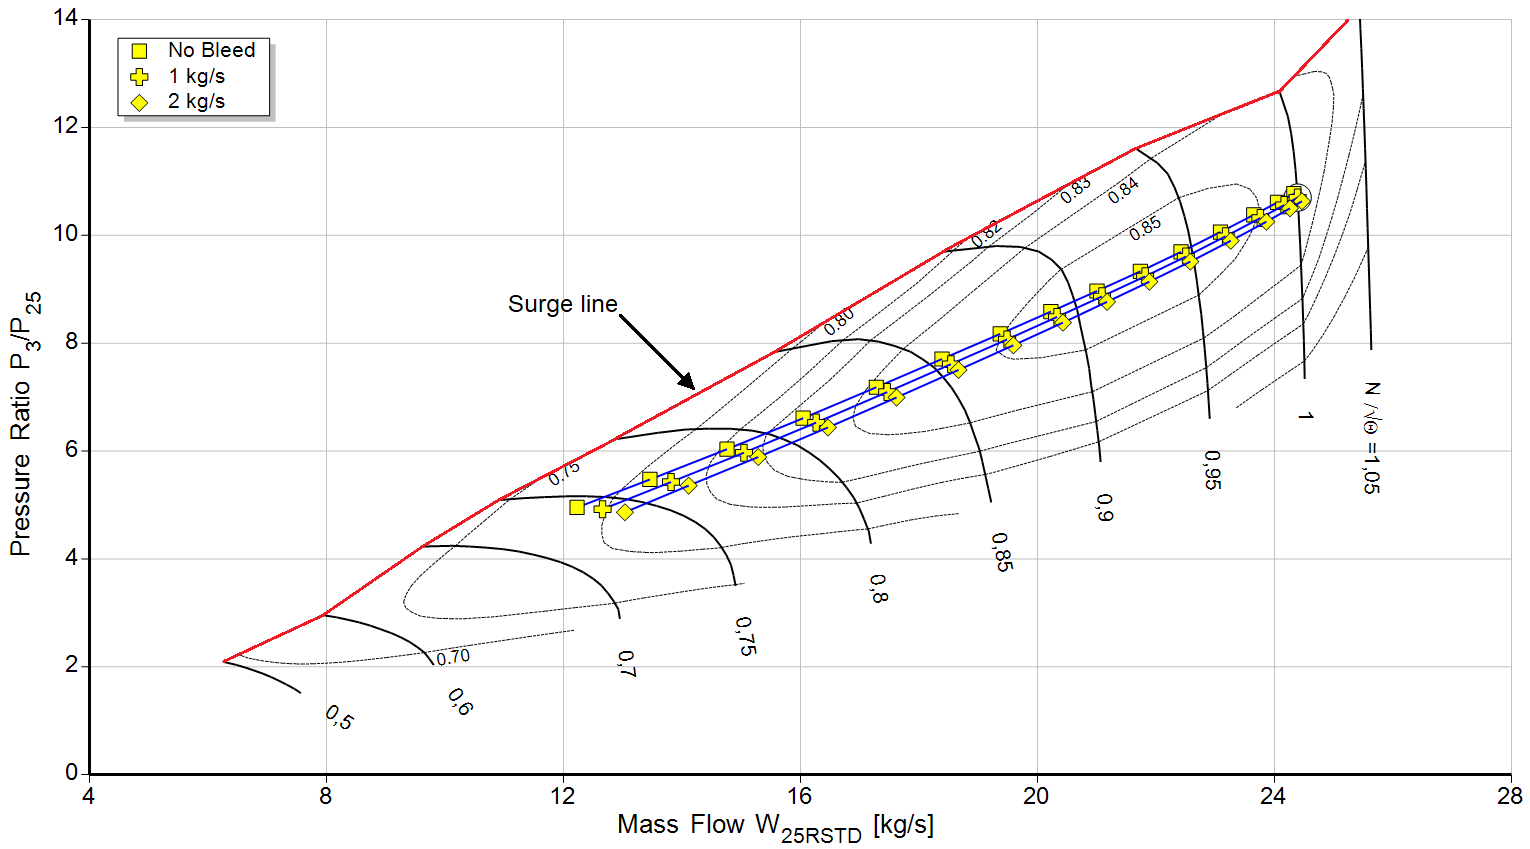
\includegraphics[width=1\textwidth]{Epictures/HPC_Map_Bleed.png}
    \caption{HPC operation lines for different bleed air flow rates.}
    \label{fig:GasTurbHPCMapBleed}
\end{figure}

\begin{figure}[hb]
    \centering
    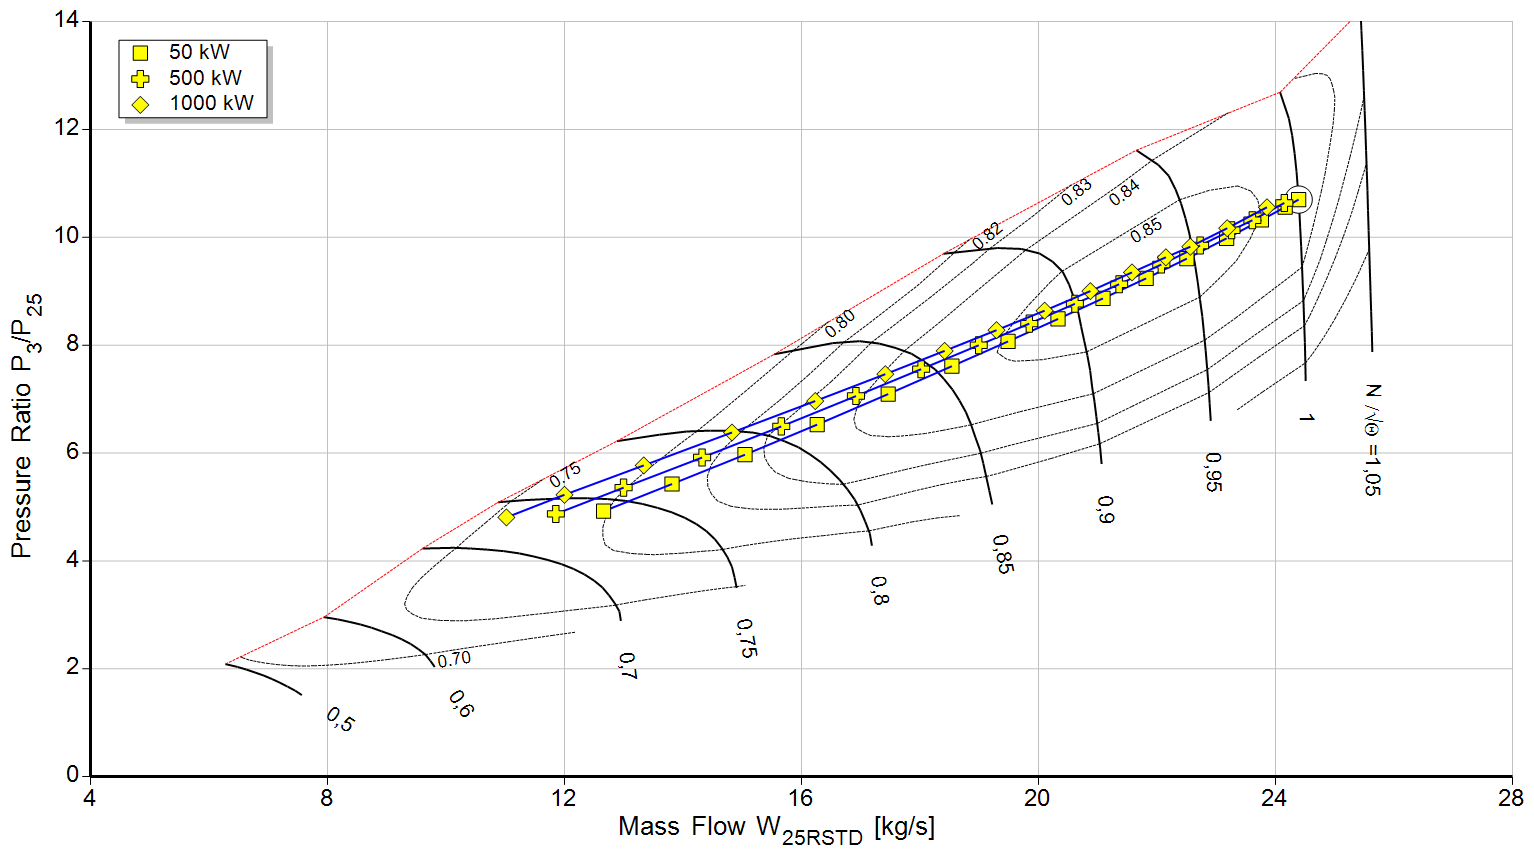
\includegraphics[width=1\textwidth]{Epictures/HPC_Map_PowerOfftakes.png}
    \caption{HPC operation lines for different power off-takes by the gearbox.}
    \label{fig:GasTurbHPCMapPower}
\end{figure}

\clearpage

\section{Engine Air Mass Flow Rate}

To calculate thrust, air mass flow rate through the engine must first be derived. The table in figure \ref{fig:CFM56-5B4GasturbTable} provides the real air mass flow rate, W2, for several different conditions. Now we need to see if it relates to anything. The goal is to use input from a flight condition to predict the engine air mass flow rate.
%\todo[inline, backgroundcolor=aqua]{Insert table CFM56-5B4GasturbTable.}

\begin{figure}[hb]
    \centering
    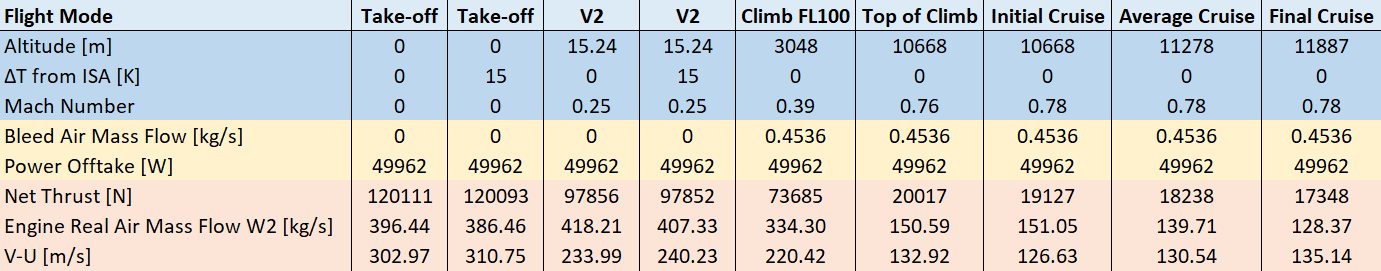
\includegraphics[width=1\textwidth]{Epictures/CFM56-5B4 GasTurb Data Fehrm.png}
    \caption{CFM56-5B4 engine simulation data. Amended from Fehrm, 2017, \cite{Fehrm2017}.}
    \label{fig:CFM56-5B4GasturbTable}
\end{figure}




%As described in the report for week 38, thrust is calculated by the relation:

%\begin{equation}
%\label{eq:Thrust}
%T = \dot{m}_a \left[ (1+f-b_3-b_{3b})V_9 +(\beta-b_{10}) V_{11} - (1+\beta) U \right]
%\end{equation}

%, where $\dot{m}_a$ is the air mass flow rate through the engine core, $V_9$ is the air exit speed from the core, $\beta$ is the bypass ratio, $V_{11}$ is the air exit speed from the fan and $U$ is the aircraft speed. $f$ is the fuel to air ratio. $b_3$, $b_{3b}$ and $b_{10}$ are bleed air ratios.\\

%Under normal conditions $f-b_3-b_{3b} \approx 0$ and $b_{10} \approx 0.01 << \beta$. For simplicity, we can ignore the small parameters. Further more, $V_9$ and $V_{11}$ are usually designed to be at high subsonic speeds, for airliners, and are nearly equal to each other, $V_9 \approx V_{11} = V$ so we can approximate equation \ref{eq:Thrust} as:

Net thrust can be approximated by:

\begin{equation}
\label{eq:ThrustSimple}
T \approx \dot{m}_a (V-U)
\end{equation}

, where $\dot{m}_a$ is the engine air mass flow rate, $V$ is the air exit speed, also called Specific Thrust, while $U$ is the flight speed, also called Specific Drag.

\subsection{Effect of Mach number on Specific Thrust}

With data from figure \ref{fig:CFM56-5B4GasturbTable}, plot of Specific Thrust and Mach number at International Standard Atmosphere, ISA $\Delta T=0$, can be seen in figure \ref{fig:STvsM}.
The linear function for Specific Thrust was derived to be:

%st = -216.0893.*m + 298.6845;
\begin{equation}
\label{eq:SpecificThrust}
V(M) = 298.68 - 216.09M \quad \mathrm{[m/s]}
\end{equation}

\begin{figure}[hb]
    \centering
    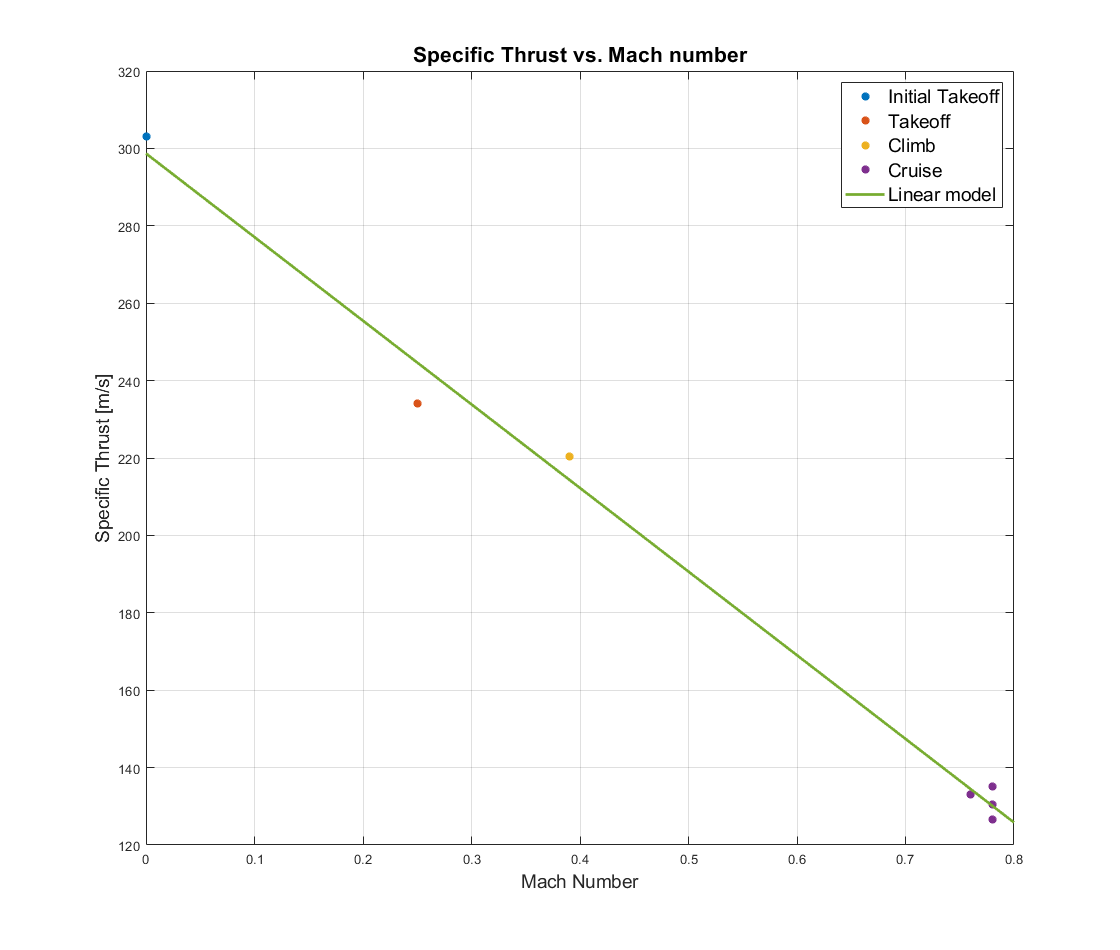
\includegraphics[width=1\textwidth]{Epictures/Specific Thrust vs. Mach number.png}
    \caption{Specific Thrust vs. Mach number.}
    \label{fig:STvsM}
\end{figure}

\clearpage

\subsection{Effect of temperature on Specific Thrust}

Conditions with different temperature deviations, $\Delta T$, from ISA are provided at altitudes close to the ground.

At M=0:

$\Delta T=0 \mathrm{K}: V = 302.97 \quad\mathrm{m/s}$

$\Delta T=15 \mathrm{K}: V = 310.75 \quad\mathrm{m/s}$\\

Change of Specific Thrust due to change in temperature is then:\\

$\frac{\Delta V}{\Delta T} =  (310.75-302.97)/15 \approx 0.5184$ at   M=0.\\

At M=0.25:

$\Delta T=0 \mathrm{K}: V = 233.99 \quad\mathrm{m/s}$

$\Delta T=15 \mathrm{K}: V = 240.23 \quad\mathrm{m/s}$\\

Gives:\\

$\frac{\Delta V}{\Delta T}  =  (240.23-233.99)/15 \approx 0.4162 $ at M=0.25.\\

%% Effect of increased temperature on Specific Thrust, Alt=0
% ISA+0, M 0: NetThrust = 302.9740 * MassFlow
% ISA+15,M 0: NetThrust = 310.7506 * MassFlow
% Change of Specific Thrust = Change of Temperature *
% (310.7506-302.9740)/15
% Delta_V = Delta_T*0.51844

% ISA+0, M 0.25: NetThrust = 233.9875 * MassFlow
% ISA+15,M 0.25: NetThrust = 240.2302 * MassFlow
% Change of Specific Thrust = Change of Temperature *
% (240.2302-233.9875)/15
% Delta_V = Delta_T*0.41618

%% Effect of increased temperature and Mach
% Altitude effect is small and has been neglected
% Delta_V = Delta_T*(0.51844 - M*0.40904)

\subsection{Effect of Mach number on $\Delta V / \Delta T$}

We have:\\

$\frac{\Delta V}{\Delta T} \approx 0.5184 $ at M=0.\\

$\frac{\Delta V}{\Delta T} \approx 0.4162 $ at M=0.25.\\

Then:\\

$\frac{\Delta V}{\Delta T}(M) \approx (0.5184 - M (0.5184-0.4162)/0.25)$\\

$\Delta V(M) \approx  \Delta T (0.5184 - 0.4090M)$\\

Specific Thrust from equation \ref{eq:SpecificThrust} can then be expanded as:

\begin{equation}
\label{eq:SpecificThrust2}
V(M,\Delta T) \approx 298.68 - 216.09M + \Delta T (0.5184 - 0.4090M) \quad \mathrm{[m/s]}
\end{equation}


\section{Validation}
To validate equation \ref{eq:SpecificThrust2}, a comparison with the data in figure \ref{fig:CFM56-5B4GasturbTable} is done by calculating the air mass flow rate by $W2 = \frac{Net Thrust}{V(M,\Delta T)} $. The result is shown in figure \ref{fig:MassFlowRateComparison}. The greatest difference occurs at condition 3, where the model made an under prediction of about 4.4\%. We can see that differences are relatively high close to the ground, but the model shows relatively good accuracy for conditions where most time is spent.

\begin{figure}[hb]
    \centering
    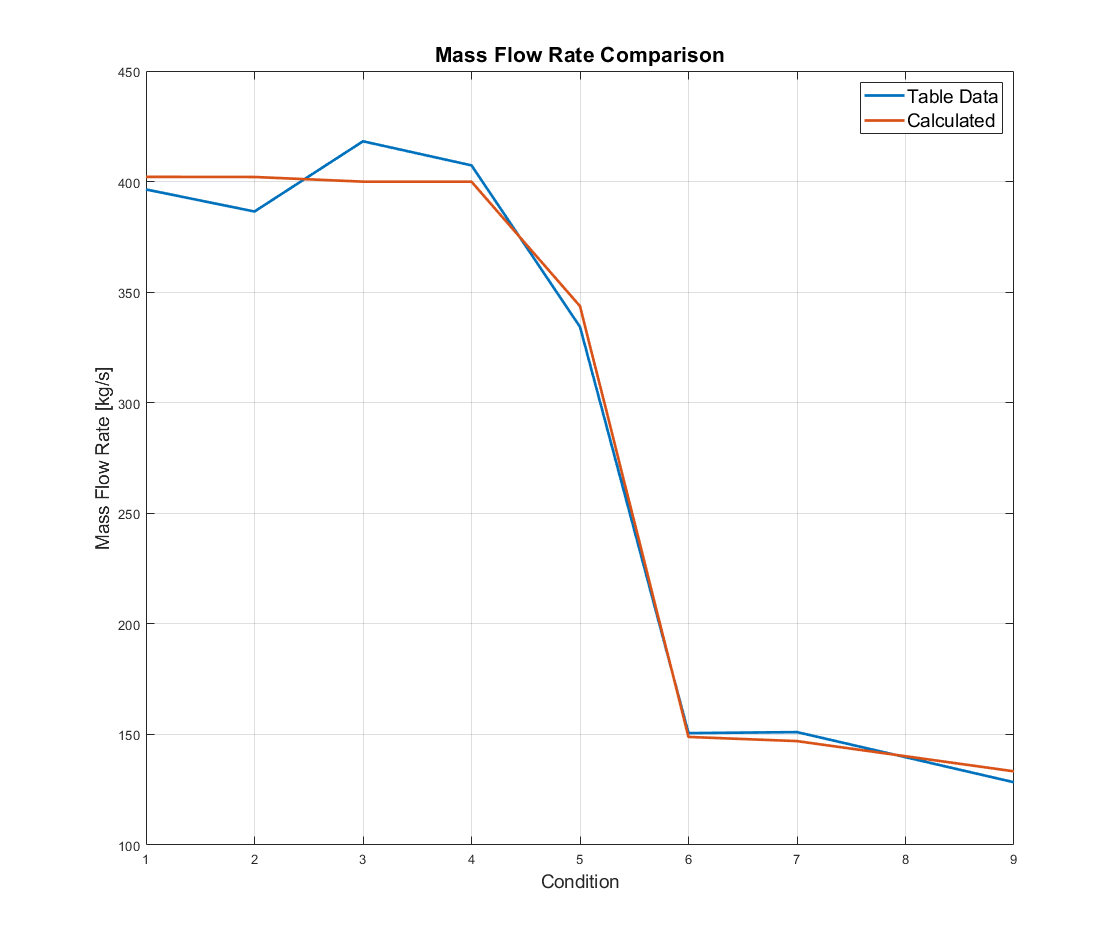
\includegraphics[width=1\textwidth]{Epictures/MassFlowRateComparison.png}
    \caption{Mass Flow Rate Comparison for different conditions.}
    \label{fig:MassFlowRateComparison}
\end{figure}


\clearpage







\section{Side note on Pneumatic \acrshort{wips}}
\todo[inline, backgroundcolor=aqua]{Engine maps. Why icing is dependent to bleed temperature.}

%########################################################################################
\cleardoublepage
\chapter{Flight dynamics}
\label{ch:flightdynamics}
%\todo[inline, backgroundcolor=aqua]{Describe why flight dynamics is important, how it affect fuel consumption.}

This chapter will show a simple 2-D flight dynamics for the airliner, see figure \ref{fig:FlightForces}. A 3-D model would be more accurate, especially for flight cases that involve much turning. An airliner does make turns, but it flies straight and uneventful for the absolute majority of the time. The 2-D model is thus considered to be good enough while requiring much less effort.

The goal is to obtain the required thrust for the aircraft to follow the flight profile.
Thrust stands for by far the most significant fuel consumption of the airliner. Thrust is also indirectly responsible for the fuel consumption of the pneumatic systems on board, through the bleed air temperature.

\begin{figure}[!ht]
    \centering
    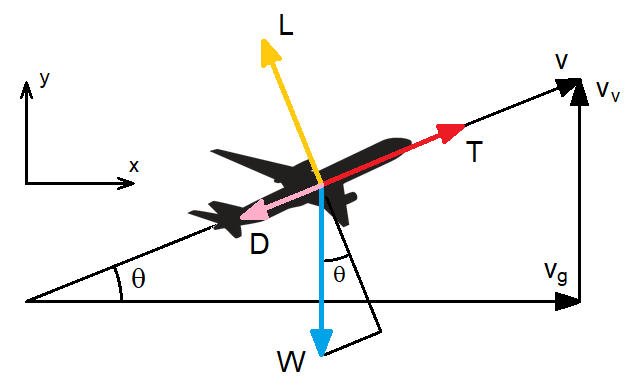
\includegraphics[width=1\textwidth]{Epictures/FlightDynamicsForces.png}
    \caption{2-D forces on the aircraft.}
    \label{fig:FlightForces}
\end{figure}

\section{Flight profile}
\label{sec:flightprofile}
%\todo[inline, backgroundcolor=aqua]{Describe flight profile, where it comes from and how it is used.}
The flight profile describes the most critical parameters that are making up the flight. It provides input to everything that is happening during a simulation.

The flight profile contains:

\begin{itemize}
  \item Time
  \item Flight mode
  \item Ground speed
  \item Altitude
  \item Distance between airports
  \item Total flight distance
  \item Temperature on ground
  \item Day or night
\end{itemize}

Time, ground speed and altitude are taken from real flight recordings, according to FlightAware \cite{flightaware} and \cite{flightaware2}. Other parameters have been added manually and compiled into a txt-file that serves as input for the simulation. Any other route can be simulated, if the flight is described as a valid flight profile and provided in a txt-file.

A flight is divided into several modes or phases. All activity of the subsystems, such as when the APU is on and flaps setting, are decided by flight mode. There are ten different modes described in the flight profile, see table \ref{table:FlightModes}.

\begin{table}[h!]
\centering
\caption{Flight modes in the flight profile.}
\begin{tabular}{ c | l }
 Mode Nr. & Description \\ 
 \hline
 \hline
 0 & Static on ground\\  
 1 & APU providing power \\
 2 & Taxi to take-off \\
 3 & Take-off \\
 4 & Climb \\
 5 & Cruise \\
 6 & Descent \\
 7 & Loitering \\
 8 & Land \\
 9 & Taxi to gate\\
\end{tabular}
\label{table:FlightModes}
\end{table}

The flight profile for the case study can be seen in figure \ref{fig:FlightProfile}.
Higher resolution figures are shown in Appendix \ref{fig:FlightAltitude}, \ref{fig:VerticalSpeed}, \ref{fig:VerticalAcceleration}, \ref{fig:FlightSpeed}, \ref{fig:FlightAcceleration} and \ref{fig:FlightMode}.
\begin{figure}[!ht]
    \centering
    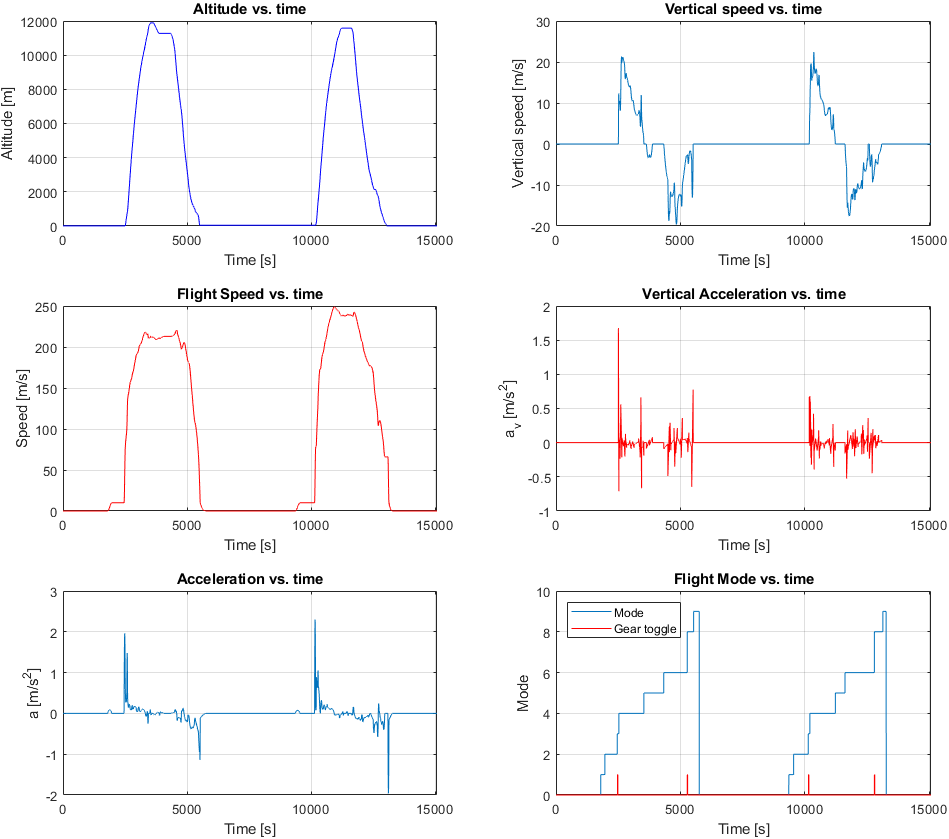
\includegraphics[width=1\textwidth]{Epictures/FlightProfile.png}
    \caption{Flight profile for a round trip flight, Copenhagen-Stockholm-Copenhagen.}
    \label{fig:FlightProfile}
\end{figure}

%\clearpage




\clearpage



\section{Weight}
\label{sec:weight}
%\todo[inline, backgroundcolor=aqua]{What is the weight of the aircraft and how is it derived?}
The weight of the aircraft is a product of its mass and gravitational constant:

\begin{equation}
\label{eq:Weight}
W = m \cdot g
\end{equation}

The mass of the aircraft is the takeoff mass minus the burned fuel:

\begin{equation}
\label{eq:ACmass}
m = m_{takeoff} - m_{fuel,burned}
\end{equation}

Takeoff mass is a sum of zero-fuel mass and fuel mass:

\begin{equation}
\label{eq:TOM}
m_{takeoff} = m_{zfm} + m_{fuel}
\end{equation}


\subsection{Zero-fuel mass}
\label{sec:zerofuelmass}
%\todo[inline, backgroundcolor=aqua]{What is zero-fuel  mass and how is it derived?}
The zero-fuel mass is the total mass of the aircraft, minus usable fuel mass. Some fuel is trapped in places where it is unusable for the engines. The unusable fuel is included in the zero-fuel mass.

Data from several airliners were compiled into a function describing the zero-fuel mass. See figure \ref{fig:ZFM}.

\begin{figure}[!ht]
    \centering
    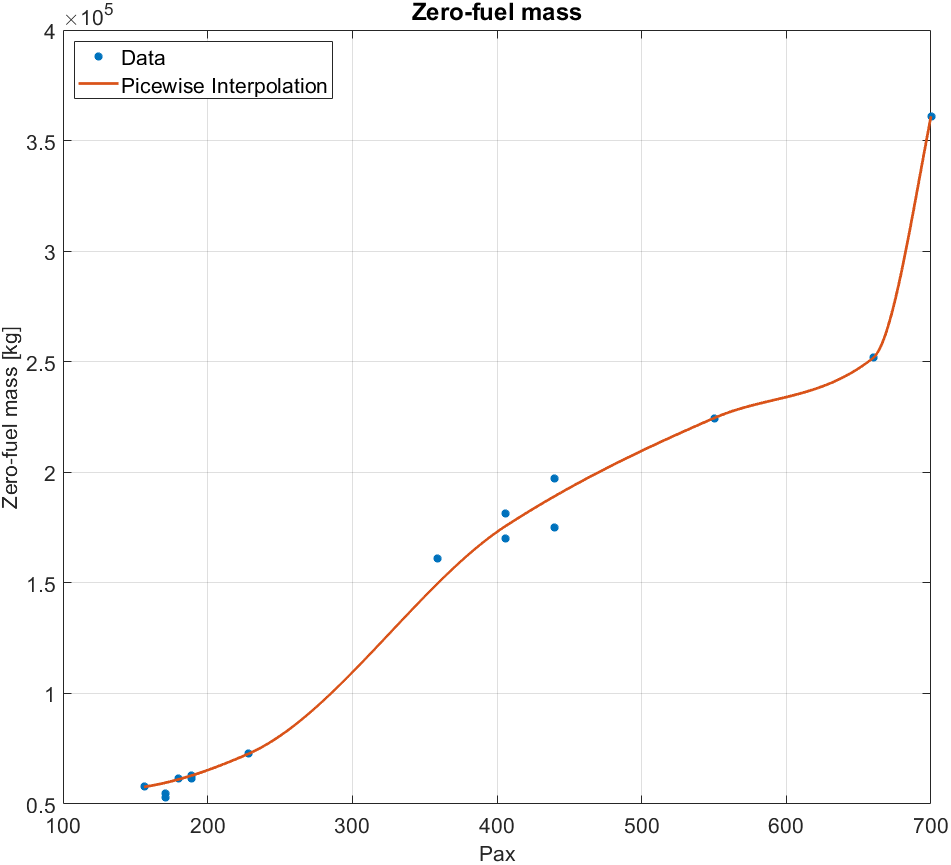
\includegraphics[width=0.7\textwidth]{Epictures/ZFM.png}
    \caption{Zero-fuel mass for a range of airliners.}
    \label{fig:ZFM}
\end{figure}

\clearpage

\subsection{Fuel mass}
\label{sec:fuelmass}
%\todo[inline, backgroundcolor=aqua]{Show how to estimate fuel mass?}
Fuel mass is used to estimate the takeoff mass of the aircraft. It is the usable fuel's initial mass and is estimated by assuming that the total fuel consumption is around 0.03 kg/(pax km), Wikipedia, \cite{WikiACFuelEconomy2021}. A safety margin of 50\% is added, and the fuel mass estimation becomes:
% Est_Fuel = 0.045*pax*dist/100;   % [kg] Estimated fuel that will be a part of takeoff mass
\begin{equation}
\label{eq:Fuelmass}
m_{fuel} = 0.045 \cdot pax \cdot dist
\end{equation}
, where $dist$ is the distance between refueling.

In reality, the safety margin can be a complex function of several parameters, such as weather and distance to other airports, but was for simplicity chosen to be a constant factor. For longer distances, when the fraction of fuel mass to total mass is more considerable, another method to estimate safety margin must be used.

\section{Lift}
\label{sec:lift}
%\todo[inline, backgroundcolor=aqua]{Show how lift is a function of mass and flight profile.}
Lift is decided by the flight profile as:
% L = W*(1+vacc)*cos(theta); % [N] Lift
%\begin{equation}
%\label{eq:Lift}
%L = W(1+a_v)cos(\theta)
%\end{equation}
\begin{equation}
\label{eq:Lift}
 L = \left\{\begin{array}{l r}
        W(1+a_v)cos(\theta) , & \text{when flying}\\
        0, & \text{on ground}
        \end{array}\right\}
\end{equation}
, where $a_v$ is the vertical acceleration and $\theta$ is the climb angle, according to figure \ref{fig:FlightForces}.

The climb angle is worked out by the relation:
% theta = asin(vspeed/speed); % [rad] Climb angle
\begin{equation}
\label{eq:Theta}
 \theta = \arcsin \frac{v_v}{v}
\end{equation}

\section{Drag}
\label{sec:drag}
\todo[inline, backgroundcolor=aqua]{What is drag and all its components?}
%\todo[inline, backgroundcolor=aqua]{Explain how drag affect fuel consumption and bleed temperature?}
Drag is the force that the aircraft is acting on the air, leaving a trail of energized air with movement and heat.

Drag can be expressed as:
 
\begin{equation}
\label{eq:Drag}
D = C_D q S
\end{equation}

, where $C_D$ is the drag coefficient, $q=\frac{\rho\cdot v^2}{2}$ is the dynamic pressure and $S$ is the wing area. Drag can be divided into parasitic drag, also called zero-lift drag, and lift-induced drag. We can express the coefficients as:

\begin{equation}
\label{eq:CD}
C_D = C_{D0} + C_{Di}%k C_L^2
\end{equation}
, where $C_{D0}$ is the parasite drag coefficient and $C_{Di}$ is the lift-induced drag coefficient.

\subsection{Zero-lift drag coefficient ($C_{D0}$)}
\label{sec:CD0}
%\todo[inline, backgroundcolor=aqua]{Show the component build-up method.}
The parasitic drag or zero-lift drag originates from viscous effects in the airflow. It is primarily a sum of skin friction and pressure drag or form drag. Protruding elements from the airframe will contribute to zero-lift drag. Flying at high subsonic speeds will generate wave drag due to compressible effect of air. Wave drag is also a part of the zero-lift drag and will be shown in section \ref{sec:wavedrag}.\\

There are several ways to estimate the zero-lift drag. The method chosen here is based on the Component Buildup Method, described by Raymer, 1992, \cite{Raymer1992} and is valid for low speeds up to the drag-divergence Mach number, $M_{DD}$. The drag-divergence Mach number is defined as the Mach number for which the wave drag coefficient has an increase of 0.002. It occurs at about M 0.84 for the A320-200, according to Scholz, 2017, \cite{Scholz2017}. This method's advantages are that it has flight condition dependency, pax-scaling properties, and is reasonably accurate. The disadvantage is that this technique requires excellent geometrical knowledge about the aircraft. A way to work around this is to study a few airliners and make functions, describing all the necessary parameters as pax functions. Although the geometry will not be perfect for every aircraft, at least we should be able to capture the scaling effect.\\

The idea with the component build-up method is to calculate the flat-plate skin friction drag coefficient ($C_f$) for each aircraft component. A Form Factor ($F_F$) is added to the function to include the pressure-drag. Influenced by the components' position, an Interference Factor, $Q$, describes how much the elements interfere with each other. How to derive $F_F$ and $Q$ are further described by Raymer. The factors that are used here are shown in table \ref{table:DragFactors}. The component drag coefficient is calculated as a product of the wetted surface area $S_{wet}$, $C_f$, $F_F$ and $Q$ divided by the wing area, $S_{wing}$. The drag coefficient for the entire aircraft is a sum of all the component drag coefficients:

\begin{equation}
\label{eq:CD0sum}
C_{D0} = \sum{C_{f,c} F_{F,c} Q_c \frac{S_{wet,c}}{S_{wing}}}
\end{equation}

, where the subscript, $c$, stands for component.

According to Anderson, 2000, \cite{Anderson2000}, the component skin friction drag coefficient for a flat plate with turbulent flow is calculated as:

\begin{equation}
\label{eq:Cfc}
C_{f,c} = \frac{0.074}{Re_c^{0.2}}
\end{equation}

The component Reynolds number is given by:

\begin{equation}
\label{eq:Rec}
Re_{c} = \frac{\rho v L_c}{\mu}
\end{equation}

, where $\rho$ $[kg/m^3]$ is the air density, $v$ $[m/s]$ is the air speed, $L_c$ $[m]$ is the effective length of the component and $\mu$ $[Ns/m^2]$ is the dynamic viscosity of air. $\rho$, $v$ and $\mu$ are all dependent on flight condition.\\

Viscosity of air is a function of temperature and is described by the Sutherland Equation, according to \cite{Sydney2005} and \cite{EngTool2003}:

\begin{equation}
\label{eq:mu}
\mu = \frac{1.458\cdot 10^{-6} \cdot T_{tot}^{1.5}}{T_{tot} + 110.4} \quad \left[ \frac{kg}{s\cdot m} \right]
\end{equation}

, where $T_{tot}$ $[K]$ is the total temperature.

\begin{table}[h!]
\centering
\caption{Form Factor, $F_F$, and Interference Factor, $Q$, for typical jet airliner components.}
\begin{tabular}{ l | l | l} 
Component & $F_F$ & $Q$\\
\hline
\hline
Wing & 1.6 & 1.0\\
Fuselage & 1.09 & 1.0\\
Tail & 1.09 & 1.04\\
Engines & 1.23 & 1.3\\
\end{tabular}
\label{table:DragFactors}
\end{table}

The geometrical properties of the aircraft components are shown in Appendix figures \ref{fig:WingAreaPax}, \ref{fig:WingChordPax}, \ref{fig:FuselageLePax}, \ref{fig:FuselageDiaPax}, \ref{fig:HtailWetPax}, \ref{fig:HtailChordPax}, \ref{fig:VtailWetPax}, \ref{fig:VtailChordPax}, \ref{fig:EngDiaSumPax} and \ref{fig:EngLePax}.

With the Component Buildup Method, combined with the mentioned geometrical properties and a typical cruise condition at M 0.8 and 11500 m, the zero-lift drag coefficient without wave drag will look like in figure \ref{fig:CD0Pax}.

\begin{figure}[!ht]
    \centering
    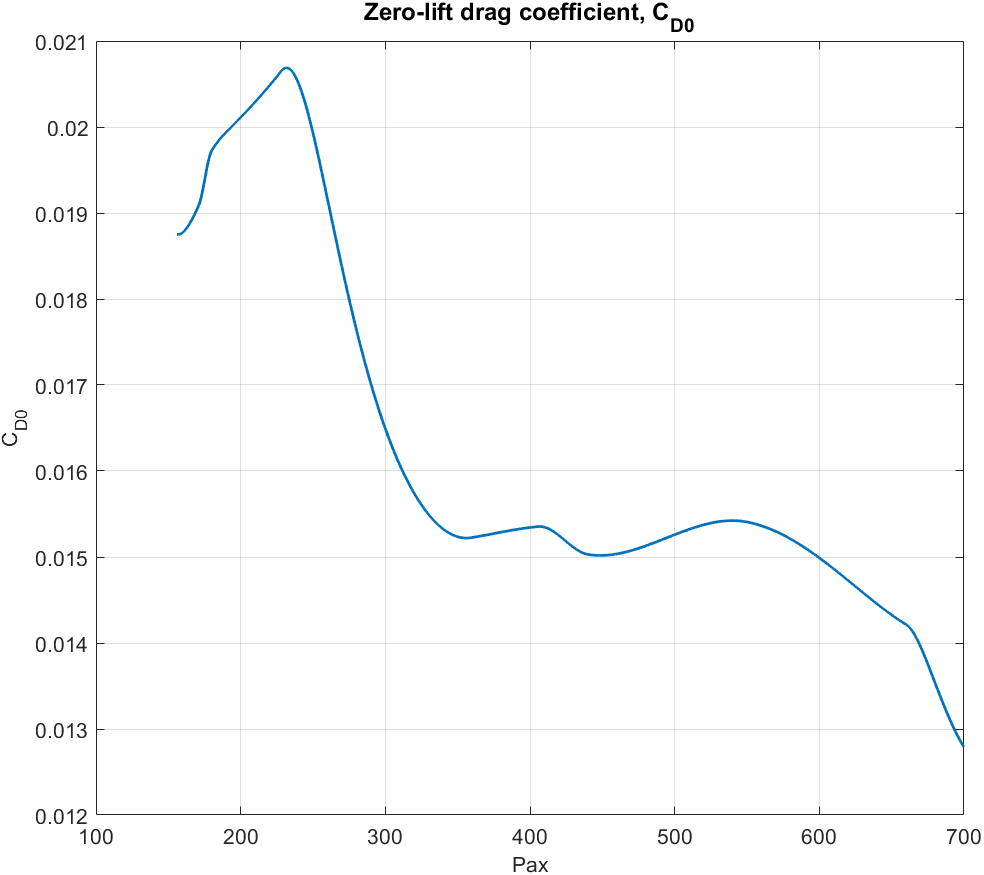
\includegraphics[width=1\textwidth]{Epictures/Zero-liftDragPax.png}
    \caption{Zero-lift drag coefficient for the airliners in this study.}
    \label{fig:CD0Pax}
\end{figure}


\subsection{Lift-induced drag coefficient ($C_{Di}$)}
\label{sec:k}
%\todo[inline, backgroundcolor=aqua]{Data from OpenAP.}

The lift-induced drag coefficient can be expressed as:
\begin{equation}
\label{eq:CDi}
C_{Di} = k C_L^2
\end{equation}
, where $C_L$ is the lift coefficient and $k$ is the \textit{drag-due-to-lift factor}.

According to the classical aerodynamic theory, this factor can be expressed as a function of wing geometry:
\begin{equation}
\label{eq:k}
k = \frac{1}{\pi \AR e}
\end{equation}
, where $\AR$ is the aspect ratio, and $e$ is the \textit{span efficiency factor} or \textit{Oswald efficiency factor}. A perfect, elliptical wing has an efficiency factor $e=1$, while typical airliners have efficiency factors close to 0.7-0.8

Many design choices can affect the \textit{span efficiency factor}, such as using different airfoil sections in the wing, applying wing twist, placement of engines, etc. Thus parameters, based on flight data, according to Sun et al., 2020, \cite{Sun2020}, will be used here. How $k$ can look like for different airliner sizes can be seen in figure \ref{fig:kPax}.

\begin{figure}[!ht]
    \centering
    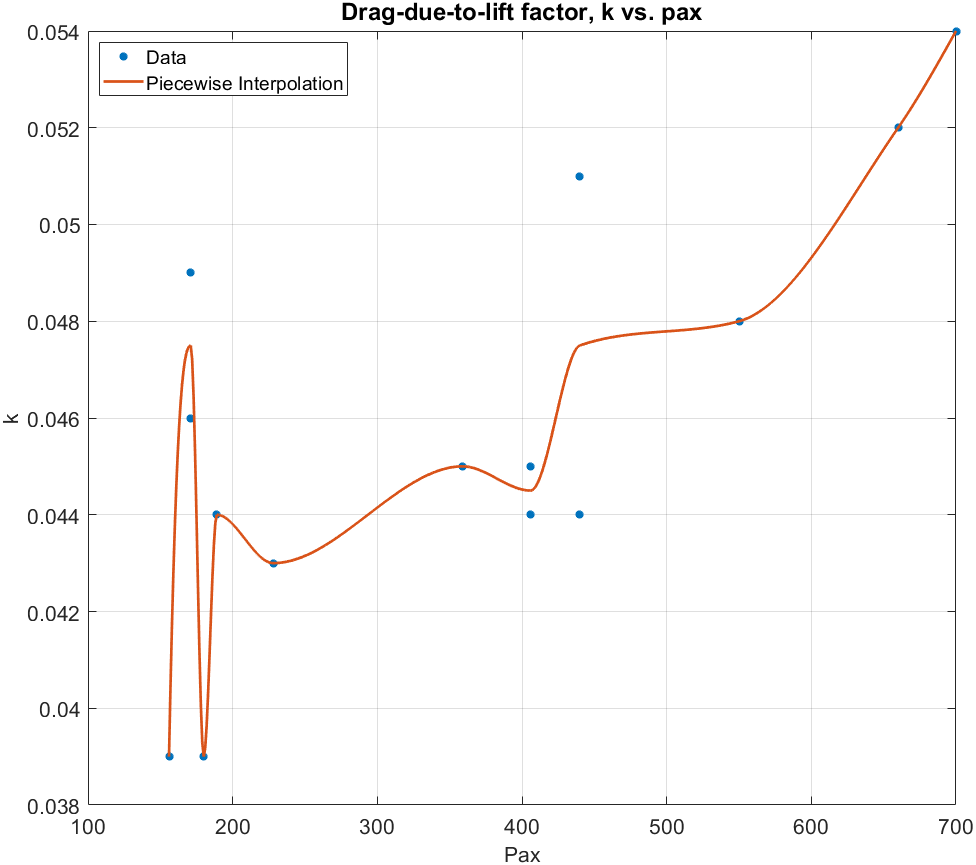
\includegraphics[width=1\textwidth]{Epictures/kvsPax.png}
    \caption{Drag-due-to-lift factor, $k$, for the airliners in this study.}
    \label{fig:kPax}
\end{figure}

%\clearpage

\subsection{Flaps effect on lift-induced drag}
\label{sec:flapsoninduceddrag}
The lift-induced drag coefficient also gets affected by the flap's deflection. According to Sun et al., 2020, \cite{Sun2020}, a model for the change of Oswald efficiency factor, $e$, is shown to be:

\begin{equation}
\label{eq:eflaps}
\Delta e_{flaps} = 0.0026 \cdot \delta_{flaps}
\end{equation}
, where $\delta_{flaps}$ $[degrees]$ is the flaps deflection.

The lift-induced drag coefficient can then be expressed as:

\begin{equation}
\label{eq:kflaps}
k_{flaps} = \frac{1}{1/k + \pi \AR \Delta e_{flaps}}
\end{equation}

, where $\AR$ is the aspect ratio of the wing.

The aspect ratio for several airliners were plotted against pax. See figure \ref{fig:ARvsPax}. 
\begin{figure}[hb]
    \centering
    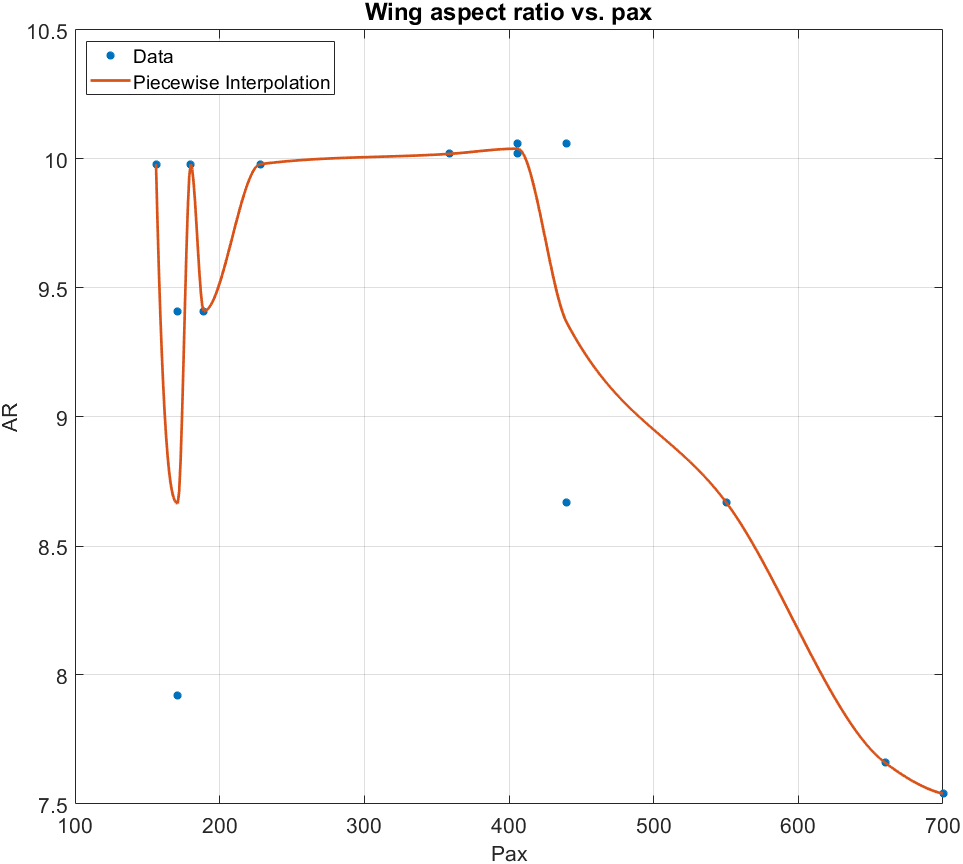
\includegraphics[width=0.7\textwidth]{Epictures/ARvsPax.png}
    \caption{Wing aspect ratio for airliners in this model.}
    \label{fig:ARvsPax}
\end{figure}




\subsection{Flaps effect on drag}
\label{sec:flapsondrag}

According to Young, 1947, \cite{Young1947}, the empirical model for the drag-increase by deployed flaps is expressed as:
 
\begin{equation}
\label{eq:dCDflapsYoung}
\Delta C_{D,flaps} = \frac{S_{fe}}{S} \cdot \delta_1(c_{fe}/c) \cdot \delta_2(\beta) \cdot \delta_3(b_{f}/b)
\end{equation}

, where $S_{fe}/S$ is the ratio between effective flaps and wing area, $c_{fe}/c$ is the ratio between effective mean flaps chord length and mean wing chord length, $c$. $\beta$ is the deflection angle, and $b_{f}/b$ is the ratio between flaps span and wingspan.

Taking the Airbus A320 as an example, by looking at the wing planform in figure \ref{fig:A320Planform}, we can roughly identify the parameters.

\begin{figure}[hb]
    \centering
    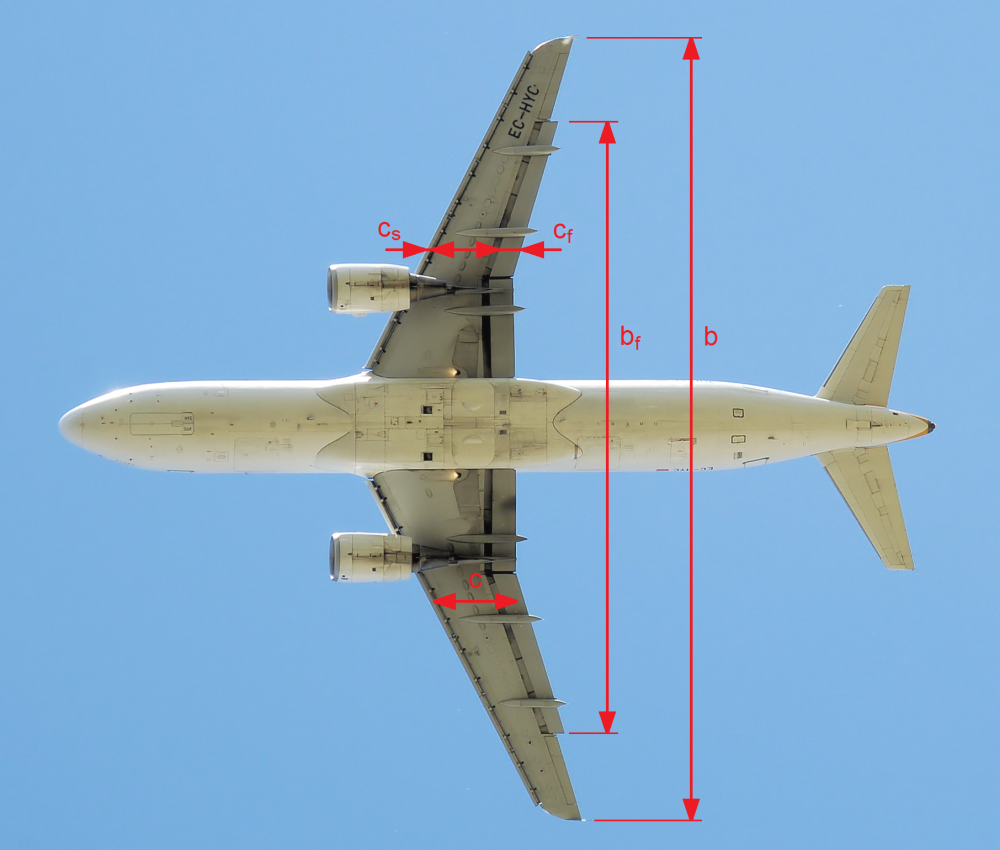
\includegraphics[width=1\textwidth]{Epictures/Iberia_a320-200_planform_Arrows.png}
    \caption{Airbus A320-200 wing planform. Amended from Wikipedia, \cite{WikiA320-2021}.}
    \label{fig:A320Planform}
\end{figure}

%\clearpage

Chord lengths of both slats and flaps are summed to obtain the effective flap chord length:

\begin{equation}
\label{eq:cfe}
c_{fe} = c_f + c_s
\end{equation}

For simplicity, since the slats have much smaller chord length than flaps, only the spanwise distribution of flaps is considered for the $b_f$.

In this case, some parameters were given by Jenkinson, 1999, \cite{Jenkinson1999}, see table \ref{table:FlapsParam}.

\begin{table}[h!]
\centering
\caption{Flaps, slats and wing parameters for Airbus A320.}
\begin{tabular}{ r c l } 
\hline
Wing area & $S$ & 122.40 $m^2$\\
Flaps area & $S_f$ & 21.10 $m^2$\\
Slats area  & $S_s$ & 12.64 $m^2$\\
Flaps span ratio & $b_f/b$ & 0.780\\
Taper ratio & $\lambda$ & 0.240\\
Average wing thickness & $t/c$ & 0.12\\
\hline
\end{tabular}
\label{table:FlapsParam}
\end{table}

The $c_{fe}/c$ ratio can then be calculated by:

$$c_{fe}/c = \frac{S_f + S_s}{S} \cdot \frac{b}{b_f} = \frac{21.10 + 12.64}{122.40} \cdot \frac{1}{0.780} \approx 0.35$$

To obtain $\delta_1$, $\delta_2$ and $\delta_3$ in function (\ref{eq:dCDflapsYoung}), a set of figures are given, see figure \ref{fig:A320Param}. Young \cite{Young1947} also introduced an approximation, $\delta_2 \approx 0.1 \cdot sin^2 \beta$. Drag increase for the A320 due to flaps can then be estimated:

$$\Delta C_{D,flaps,20\degree} = \frac{21.10 + 12.64}{122.40} \cdot 2.28 \cdot 0.88 \cdot 0.1 \cdot sin^2 20\degree \approx 0.0065$$
$$\Delta C_{D,flaps,40\degree} = \frac{21.10 + 12.64}{122.40} \cdot 2.28 \cdot 0.88 \cdot 0.1 \cdot sin^2 40\degree \approx 0.0229$$\\

We can compare this drag increase with the method, provided by Sun et al., 2020, \cite{Sun2020}, for the A320:

\begin{equation}
\label{eq:CDflapsOpenAP}
\text{(OpenAP)} \quad \Delta C_{D,flaps} = 0.9 \cdot \left(\frac{c_{fe}}{c}\right)^{1.38} \cdot \frac{S_{fe}}{S} \cdot sin^2 \beta \approx 0.211 \cdot \frac{S_{fe}}{S} \cdot sin^2 \beta
\end{equation}

\begin{equation}
\label{eq:CDflapsYoung}
\text{(Young)} \quad \Delta C_{D,flaps} = \delta_1(c_{fe}/c)\cdot \delta_3(b_f/b) \cdot \frac{1}{10}\cdot\frac{S_{fe}}{S} \cdot sin^2 \beta \approx 0.200\cdot\frac{S_{fe}}{S} \cdot sin^2 \beta
\end{equation}
, where the effective flaps area is $S_{fe} = S_f+S_s$.

Judging by the similarities, it should be safe to use both methods, though the method described by Young was chosen for this study. A simplification was made using the same flaps layout as for the A320 for every aircraft in the model.

\begin{figure}[hb]
    \centering
    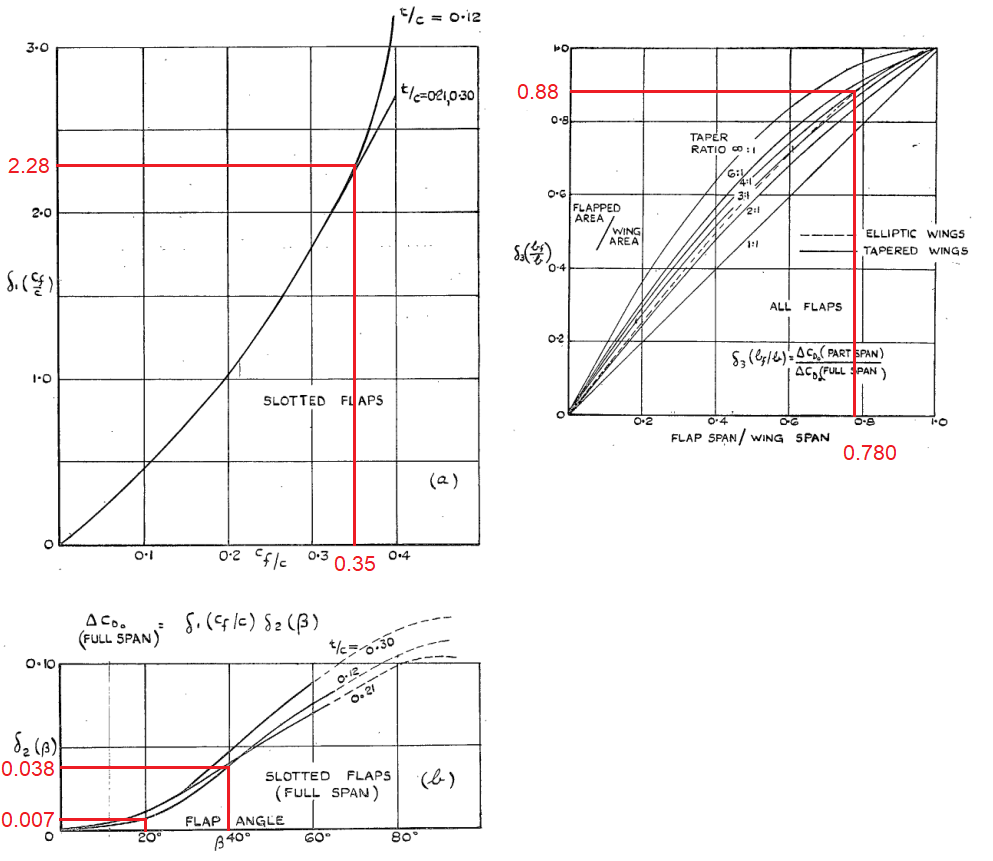
\includegraphics[width=1\textwidth]{Epictures/SlottedFlapsParametersA320-Young.png}
    \caption{Parameters for slotted flaps. Amended from Young, 1947, \cite{Young1947}.}
    \label{fig:A320Param}
\end{figure}

%\clearpage

\subsection{Effect of landing gear on drag}
\label{sec:landinggearondrag}
Not much could be found about drag, induced by extended undercarriage, other than that it adds a significant amount to the total drag. The undercarriage is composed of many non-aerodynamic shapes, see figure \ref{fig:DC8Gear}, and combined with extended flaps, the flow is highly three dimensional and complicated. Interference with the fuselage and wing is severe. Therefore, estimations of the drag contribution by the undercarriage are very dependent on experimental data. Very little data are publicly available. On the other hand, the duration of deployed landing gear is relatively short (when the plane is moving), compared to the total flight time and the uncertainty should not make a great impact on the total fuel consumption.

\begin{figure}[hb]
    \centering
    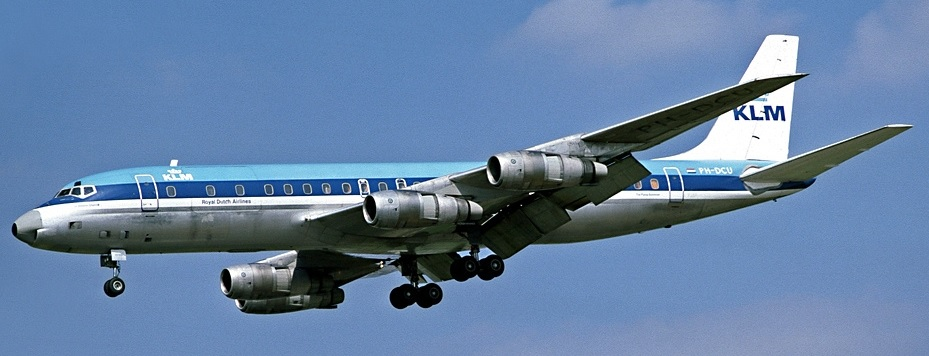
\includegraphics[width=1\textwidth]{Epictures/Undercarriage_Flaps_Douglas_DC-8-55CF.jpg}
    \caption{Douglas DC-8 with deployed undercarriage and flaps, Wikipedia \cite{WikipediaDC8}.}
    \label{fig:DC8Gear}
\end{figure}

%\begin{figure}[hb]
%    \centering
%    \includegraphics[width=1\textwidth]{Epictures/Boeing 777_Landinggear_flowfield.jpg}
%    \caption{Air velocity profile around the nose landing gear of Boeing 777, NASA \cite{NASAnoise2017}.}
%    \label{fig:B777GearCFD}
%\end{figure}

%\subsubsection{Landing gear drag estimations}
According to Sun et al., 2020, \cite{Sun2020} (which refers to Mair et al., 1992, \cite{Mair1992}), added drag by deployed landing gear for an airliner can be estimated by the expression:

\begin{equation}
\label{eq:OpenAPGearDrag}
\Delta C_{D,gear} = \frac{W}{S} K_{gear} m_{max}^{-0.215}
\end{equation}

, where $\frac{W}{S}$ is the wing loading in $[N/m^2]$, $m_{max}$ is aircraft's maximum weight in $[kg]$. Depending on the flaps deflection, the factor, $K_{gear}$, is empirically derived according to table \ref{table:Kgear}.

\begin{table}[h!]
\centering
\caption{$K_{gear}$ parameter depending on flaps deflection, OpenAP \cite{Sun2020}.}
\begin{tabular}{ r | l } 
\hline
Flaps setting & $K_{gear}$ \\
\hline
No deflection (Taxi) &  $5.81 \cdot 10^{-5}$\\
Medium deflection (Takeoff)  & $4.49 \cdot 10^{-5}$ (Interpolated)\\
High deflection (Landing) & $3.16 \cdot 10^{-5}$\\
\hline
\end{tabular}
\label{table:Kgear}
\end{table}

The lower value of drag for higher flaps deflection is explained by the reduction of relative air velocity at the undercarriage when the flaps angle is increased.

Taking the Douglas DC-8 as an example and with equation (\ref{eq:OpenAPGearDrag}), the additional drag by extended landing gear can be calculated:

$$ \text{Taxi:       } \quad  \Delta C_{D,gear} = \frac{154720 \cdot 9.81}{269.9} \cdot 5.81 \cdot 10^{-5} \cdot  154720^{-0.215} \approx 0.025$$

$$ \text{Takeoff:  } \quad  \Delta C_{D,gear} = \frac{154720 \cdot 9.81}{269.9} \cdot 4.49 \cdot 10^{-5} \cdot  154720^{-0.215} \approx 0.019$$

$$ \text{Landing:} \quad  \Delta C_{D,gear} = \frac{154720 \cdot 9.81}{269.9} \cdot 3.16 \cdot 10^{-5} \cdot  154720^{-0.215} \approx 0.014$$\\

Test flight data of the DC-8 shows that OpenAP over estimate this drag rise, see figure \ref{fig:DC8Measured}.

\begin{figure}[hb]
    \centering
    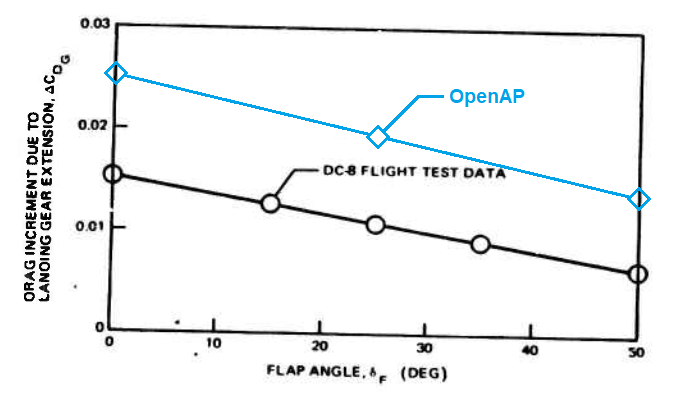
\includegraphics[width=0.8\textwidth]{Epictures/DC-8 FlightMeasuredLandingGearDragIncrementVsFlapsAngle.png}
    \caption{Flight measured undercarriage drag increment for the DC-8,according to Callaghan, 1974, \cite{Callaghan1974}.}
    \label{fig:DC8Measured}
\end{figure}

\clearpage

Other methods to estimate drag are the component build-up method and Computational Fluid Dynamics (CFD). Both these methods are used by Onaindia, 2019, \cite{Onaindia2019}, to predict undercarriage drag on the BAe Jetstream 31, figure \ref{fig:BAeJ31}. The CFD model did not include the effect of flaps nor the propeller slipstream. The latter can be favourable to produce a result similar to jet airliners.

\begin{figure}[hb]
    \centering
    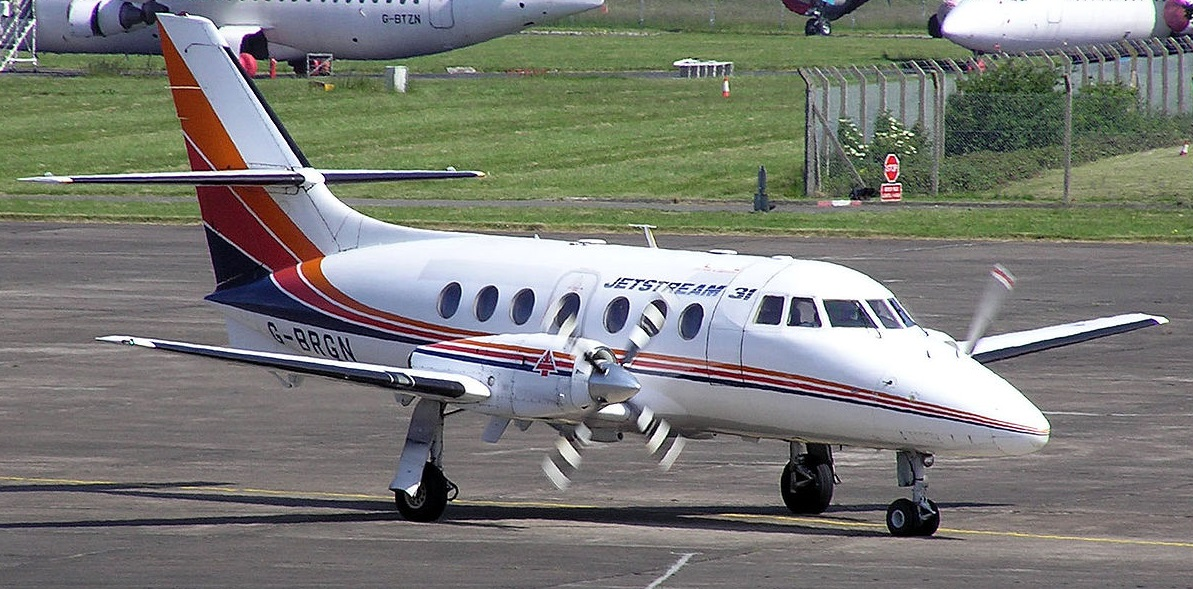
\includegraphics[width=1\textwidth]{Epictures/1280px-Jetstream31.jpg}
    \caption{Taxing BAe Jetstream 31, Wikipedia, \cite{WikipediaBAeJ31}.}
    \label{fig:BAeJ31}
\end{figure}

%\begin{figure}[hb]
%    \centering
%    \includegraphics[width=1\textwidth]{Flow past main gear BAeJ31.png}
%    \caption{Flow past the main landing gear, M=0.25 $\alpha=7\degree$, Onaindia \cite{Onaindia2019}.}
%    \label{fig:BAeJ31CFD}
%\end{figure}


This aircraft may not have the same proportion as a conventional jet airliner. We should also consider the propeller slipstream on the main landing gear, leading to a relatively high drag coefficient for the measured data, compared to calculations. Figure \ref{fig:BAeJ31Compare} shows the drag increment by the undercarriage for the BAe Jetstream 31. The component build-up method, used by Onaindia, comes from ESDU 79015 \cite{ESDU79015}.\\

It is hard to conclude which method is best. There are too little data available to validate the calculations. The component build-up method seems to get close to experimental data, at least when the attack angle is small. The method proposed by Sun et al., 2020, \cite{Sun2020}, has a compelling balance between ease of use and accuracy and is therefore chosen for the simulation.

\begin{figure}[hb]
    \centering
    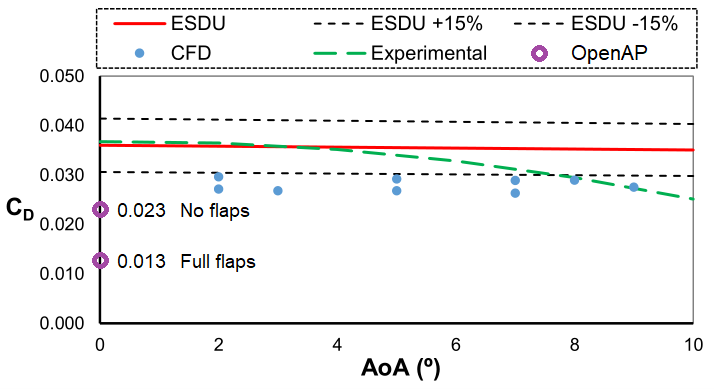
\includegraphics[width=1\textwidth]{Epictures/BAe Jetstream 31 Gear Drag.png}
    \caption{Comparison between different methods for the added drag by the undercarriage on BAe Jetstream 31. Amended from Onaindia, 2019, \cite{Onaindia2019}.}
    \label{fig:BAeJ31Compare}
\end{figure}

\clearpage

\subsection{Wave drag}
\label{sec:wavedrag}
According to Scholz, 2017, \cite{Scholz2017}, the wave drag can be estimated as:

\begin{equation}
\label{eq:CDwaveScholz}
\Delta C_{D,wave} = cos^3 \Lambda_{c/4} \cdot A \cdot tan \left( B \frac{M}{M_{crit}} - B \right)
\end{equation}

, where $\Lambda_{c/4}$ is the wing quarter chord sweep angle, $M$ is the flight Mach number, $M_{crit}$ is the critical Mach number, $A$ and $B$ are aircraft specific parameters and are given for a small number of aircraft. If they are not known, then "average" values for transport aircraft can be used: $A = 0.001272$, $B = 3.477$.

For the Boeing B727-200, the parameters are given in table \ref{table:B727Param}.

\begin{table}[h!]
\centering
\caption{Boeing B727-200 parameters , Scholz \cite{Scholz2017}, Boeing \cite{Boeing727-2007}.}
\begin{tabular}{ r l } 
\hline
A & 0.000766\\
B & 5.257\\
$M_{crit}$ & 0.70\\
$\Lambda_{c/4}$ & 32$\degree$\\
\hline
\end{tabular}
\label{table:B727Param}
\end{table}

A plot of equation (\ref{eq:CDwaveScholz}) for the B727-200, together with the OpenAP \cite{Sun2020} method and  experimental data is shown in figure \ref{fig:dCDwaveB727}. The experimental data were extracted from figure \ref{fig:dCDwaveRoskam}. We can see that the method proposed by Scholz follows well with the measured data. OpenAP shows the better result at a very narrow speed region, close to the critical Mach number, but diverges heavily from the measured data at the rest of the speeds, especially at cruise.

For the Airbus A320, the parameters are shown in table \ref{table:A320Param} and the plot can be seen in figure \ref{fig:dCDwaveA320}.

\begin{table}[h!]
\centering
\caption{Airbus A320 parameters, according to Scholz, 2017, \cite{Scholz2017} and Jenkinson, 1999, \cite{Jenkinson1999}.}
\begin{tabular}{ r l } 
\hline
A & 0.000885\\
B & 3.734\\
$M_{crit}$ & 0.632\\
$\Lambda_{c/4}$ & 25$\degree$\\
\hline
\end{tabular}
\label{table:A320Param}
\end{table}


As we can see, Scholz's method is more relevant and will be used in this work. The "average" values for $A$ and $B$ will apply for all airliners since we don't know the specific values for all aircraft. The wing quarter chord sweep angle, $\Lambda_{c/4}$, and critical Mach number, $M_{crit}$, for all airliners in the model can be seen in Appendix \ref{fig:WingSweepPax} and \ref{fig:McritPax}.

\begin{figure}[hb]
    \centering
    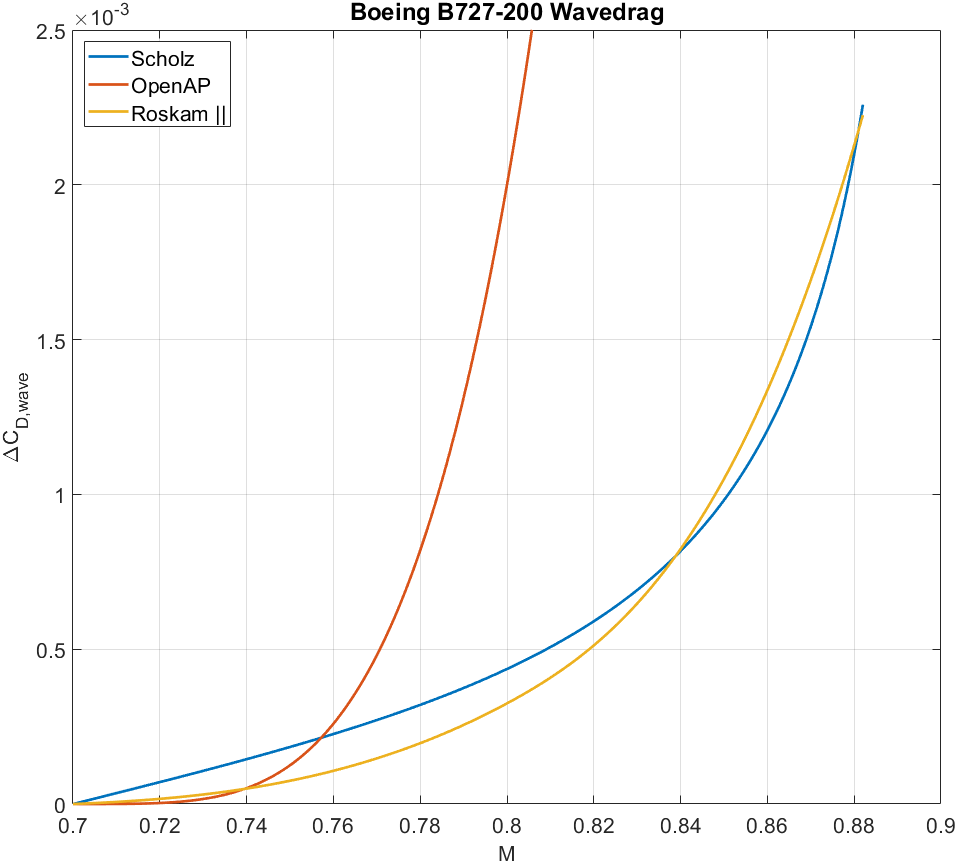
\includegraphics[width=0.7\textwidth]{Epictures/B727WaveDrag.png}
    \caption{Boeing B727-200 wave drag comparison.}
    \label{fig:dCDwaveB727}
\end{figure}

\begin{figure}[hb]
    \centering
    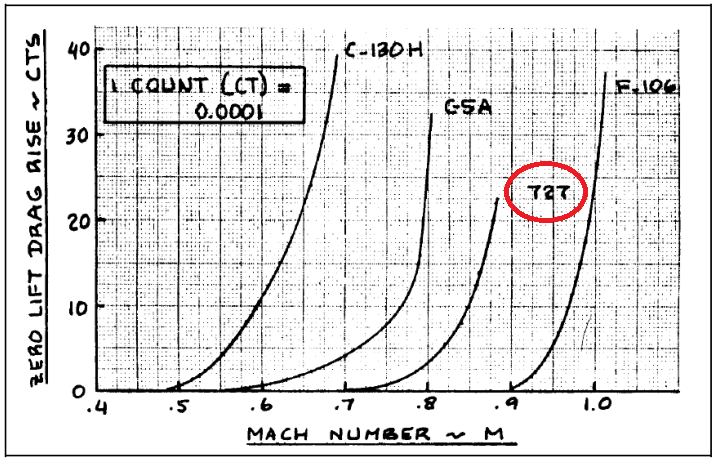
\includegraphics[width=0.7\textwidth]{Epictures/Wave Drag Roskam 2.png}
    \caption{Wave drag curves for some aircraft. Amended from Scholz \cite{Scholz2017} (originated from Roskam II, 1985).}
    \label{fig:dCDwaveRoskam}
\end{figure}

\begin{figure}[hb]
    \centering
    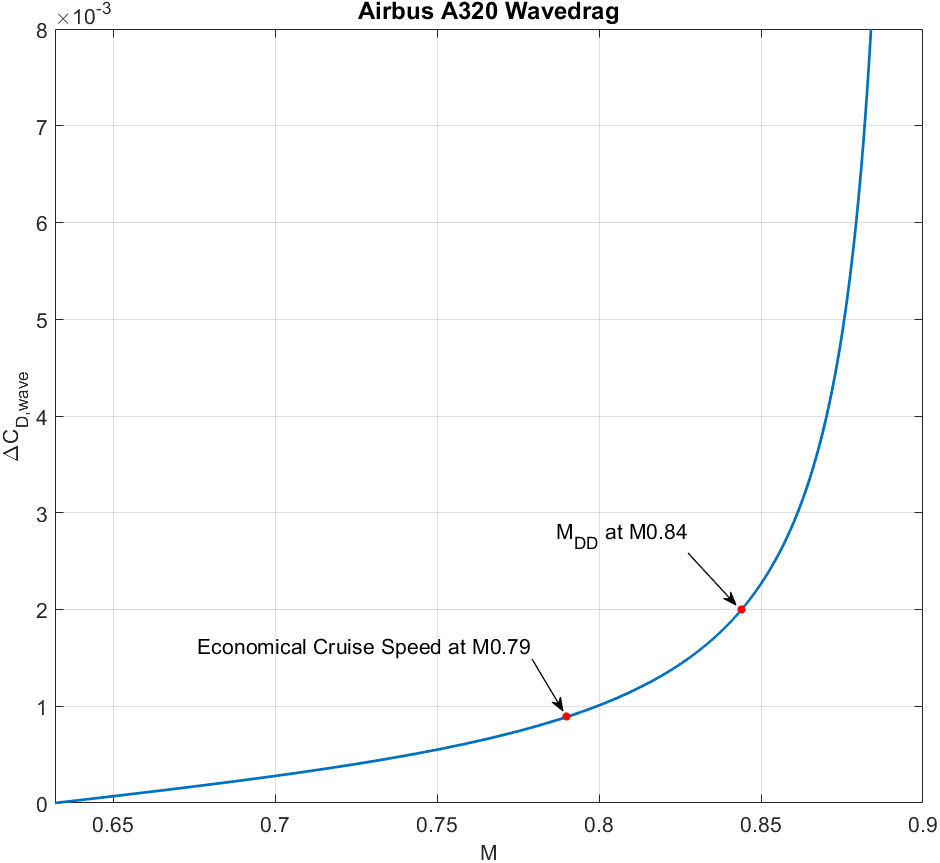
\includegraphics[width=1\textwidth]{Epictures/A320WaveDrag.png}
    \caption{Airbus A320 wave drag with the Drag Divergence Mach number and Economical Cruise Speed.}
    \label{fig:dCDwaveA320}
\end{figure}

\clearpage


\subsection{Sum of all drag}
\label{sec:sumdrag}
By including all effects, that is mentioned here, on drag, the zero-lift drag coefficient can be calculated as:

\begin{equation}
\label{eq:CD0all}
C_{D0,all} = C_{D0} + \Delta C_{D,flaps} + \Delta C_{D,gear} + \Delta C_{D,wave}
\end{equation}\\

The drag coefficient from equation (\ref{eq:CD}) can then be rewritten:

\begin{equation}
\label{eq:CDall}
C_{D,all} = C_{D0,all} + k_{flaps} C_{L}^2
\end{equation}\\

The total drag can finally be expressed as:

\begin{equation}
\label{eq:Dall}
D = C_{D,all} q S
\end{equation}\\

%\clearpage


\section{Thrust}
\label{sec:thrust}
%\todo[inline, backgroundcolor=aqua]{How is the required thrust calculated?}
According to figure \ref{fig:FlightForces}, the Required Net Thrust can simply be calculated by:
% Flying
% T = D + W*sin(theta) + acc*W; % [N] Net Thrust
\begin{equation}
\label{eq:ThrustFly}
T = D + W \left( \sin \theta + \frac{a}{g} \right)
\end{equation}

, where $a$ is the acceleration of the aircraft.

When taxiing, thrust is expressed as:
% Taxi
% T = 0.02*W + acc*W/g; % Rolling resistance and acceleration
\begin{equation}
\label{eq:ThrustTaxi}
T = W \left( C_{rr} + \frac{a}{g} \right)
\end{equation}
, where $C_{rr}$ is the coefficient of rolling resistance and is set to 0.02, according to \cite{EngTool2008}.

Maximum Net Thrust is dependent on the Maximum Takeoff Mass and is shown for the airliners in this study in figure \ref{fig:maxTvsMTOM}.
Minimum Net Thrust is dependent on the engine maps, which are shown in section \ref{sec:cfm56-5b}.

\begin{figure}[hb]
    \centering
    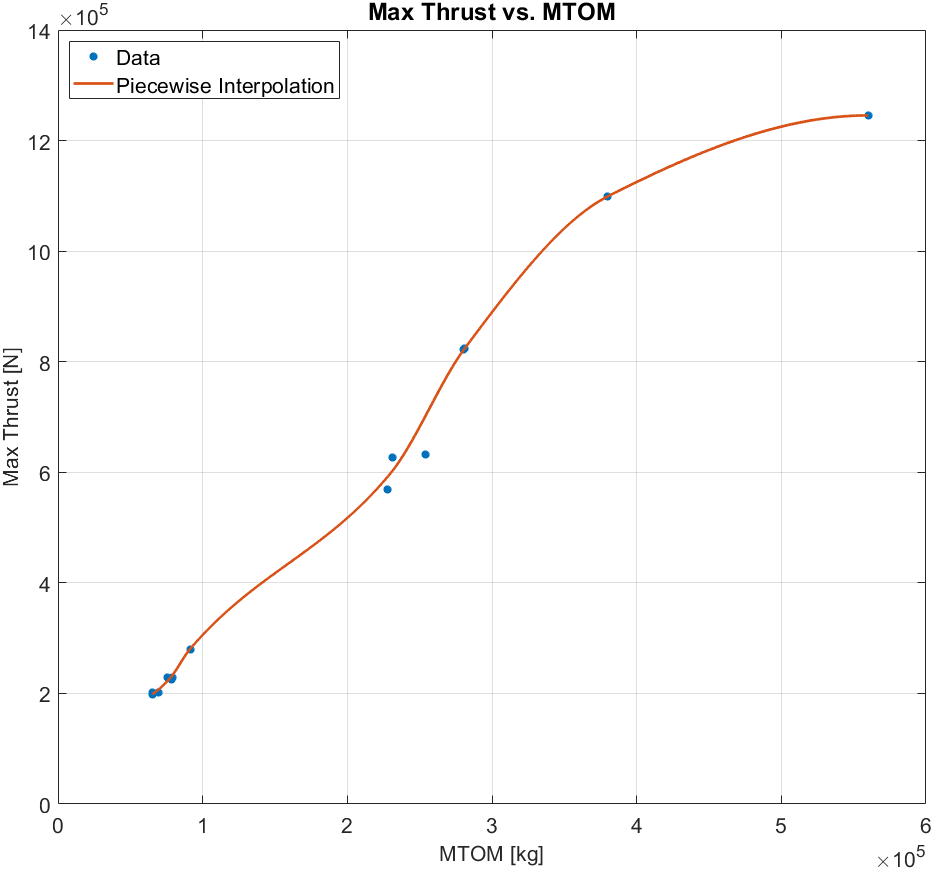
\includegraphics[width=1\textwidth]{Epictures/MaxTvsMTOM3.png}
    \caption{Maximum Net Thrust vs. Maximum Takeoff Mass for the airliners in this study.}
    \label{fig:maxTvsMTOM}
\end{figure}

%\clearpage

%########################################################################################
\cleardoublepage
\chapter{Thrust Specific Fuel Consumption (TSFC)}
\label{ch:tsfc}
%\todo[inline, backgroundcolor=aqua]{Show how TSFC was derived.}
The engine's Thrust Specific Fuel Consumption (TSFC) is dependent on several factors, such as engine type, bypass ratio, temperature, speed etc. According to Scholz et al., 2013, \cite{Scholz2013}, the TSFC of modern airliners jet's engines in cruise is around 16 mg/Ns, based on JET-A1 as fuel. Very advanced engines can have a value as low as 14 mg/Ns.
An estimation of TSFC as function of speed and temperature can be shown to be:

\begin{equation}
\label{eq:TSFC}
TSFC=(1.13 \cdot 10^{-5} + 1.25 \cdot 10^{-5} \cdot M) \cdot \sqrt{\frac{T_{amb}}{T_0}} \quad \textrm{[kg/Ns]}
\end{equation}

, where $M$ is the flight Mach number. $T_{amb}$ is the ambient temperature at altitude. $T_0=288$ K.\\

TSFC for a flight can be seen in figure \ref{fig:TSFC}.

\begin{figure}[h]
    \centering
    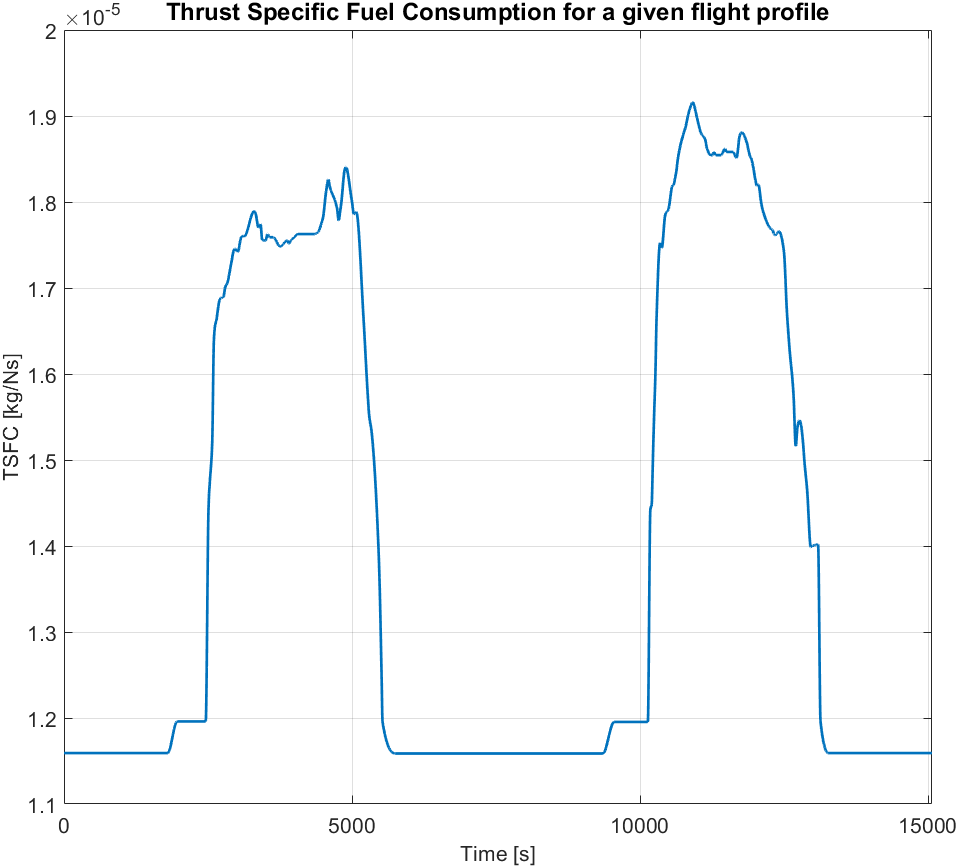
\includegraphics[width=1\textwidth]{Epictures/TSFC.png}
    \caption{Thrust Specific Fuel Consumption for a round trip flight between Copenhagen and Stockholm.}
    \label{fig:TSFC}
\end{figure}

%########################################################################################
\cleardoublepage
\chapter{Shaft power to fuel consumption}
\label{ch:shaftpowertofuel}
%\todo[inline, backgroundcolor=aqua]{Show how all kinds of secondary power can be converted to shaft power.}
%\todo[inline, backgroundcolor=aqua]{Show how shaft power can be converted to fuel consumption.}
This chapter will show how shaft power extracted from the engine can be transformed into fuel consumption. We have already seen how bleed-air is related to shaft power in section \ref{subsubsec:ACMShaftPower}. There are also mechanical ways to extract energy from the engine, going through the accessory gearbox connected to one or more of the engine's shaft. Electric generators, hydraulics pumps and fuel pumps are a few examples of units attached to the accessory gearbox.

Figure \ref{fig:PowerFlow} shows how secondary power, which is all power that is not used for thrust, is related to fuel consumption.

\begin{figure}[h]
    \centering
    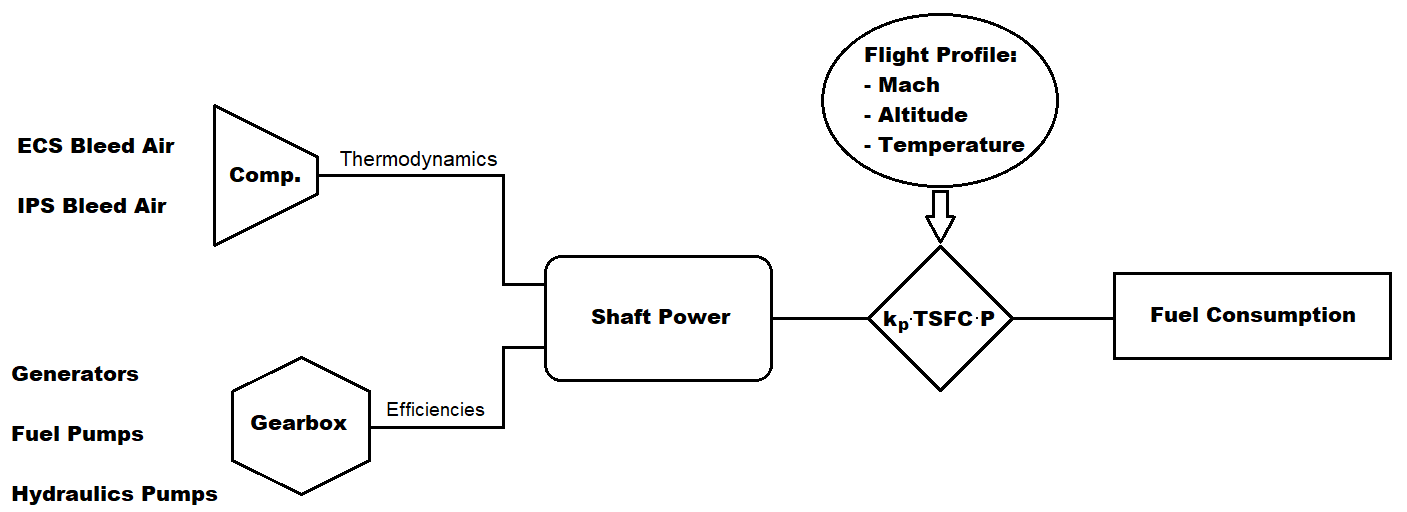
\includegraphics[width=1\textwidth]{Epictures/PowerFlow.png}
    \caption{Chart showing how secondary power is related to fuel consumption.}
    \label{fig:PowerFlow}
\end{figure}

\clearpage

\section{Shaft power factor}
\label{sec:ShaftPowerFactor}
Fuel mass flow due to thrust can be expressed as:

\begin{center}
$\dot{m}_{fuel,T} = TSFC \cdot T$
\end{center}

Shown by Scholz et al., 2013,\cite{Scholz2013}, shaft power off-takes cause a change in fuel consumption by $\Delta TSFC$. Fuel flow due to the off-take is then:

\begin{equation}
\label{eq:deltaTSFC}
\dot{m}_{fuel,P} = \Delta TSFC \cdot T
\end{equation}

By introducing shaft Power Specific Fuel Consumption, we can write:

\begin{equation}
\label{eq:PSFC}
\dot{m}_{fuel,P} = PSFC \cdot P
\end{equation}
, where $P$ is the shaft power off-take.

Combine \ref{eq:deltaTSFC} and \ref{eq:PSFC} gives:

\begin{center}
$PSFC \cdot P = \Delta TSFC \cdot T$
\end{center}

Divide by TSFC to get the relation:

$$\frac{PSFC}{TSFC} \cdot P = \frac{\Delta TSFC}{TSFC} \cdot T$$

It was observed that

\begin{itemize}
  \item $\Delta TSFC$, due to shaft power off-takes is almost proportional to $TSFC$.
  \item $\Delta TSFC$ is rather proportional to $P$/$T$ than to $P$; i.e. the same shaft power taken from an engine with high thrust does not consume as much fuel as taken from the same engine during low thrust.
\end{itemize}

A shaft power factor $k_P$ is then defined as:

$$\frac{\Delta TSFC}{TSFC} = k_P \cdot \frac{P}{T}$$

$$k_P = \frac{PSFC}{TSFC} \quad \textrm{[N/W]}$$

$$k_P = \frac{\Delta TSFC / TSFC}{P / T}$$

When $k_P$ is known, fuel consumption due to shaft power off-take can be calculated with:

\begin{equation}
\dot{m}_{fuel,P} = k_P \cdot TSFC \cdot P \quad \textrm{[kg/s]}
\end{equation}

Studies of data for several engines in cruise flight showed an average value $k_P = 0.00226$ N/W.

An approximation of $k_P$ for similar turbofan engines as function of Mach number, $M$, and altitude, $h$, was derived to be:

\begin{equation}
\label{eq:kp}
k_P = 0.0057 + 4.60 \cdot 10^{-8} h - 0.0106 M - 4.44 \cdot 10^{-13} h^2 + 1.85 \cdot 10^{-7} h M + 0.0049 M^2
\end{equation}

A plot of how $k_P$ can look like during a flight is shown in figure \ref{fig:ShaftPowerFactor}.

\begin{figure}[h]
    \centering
    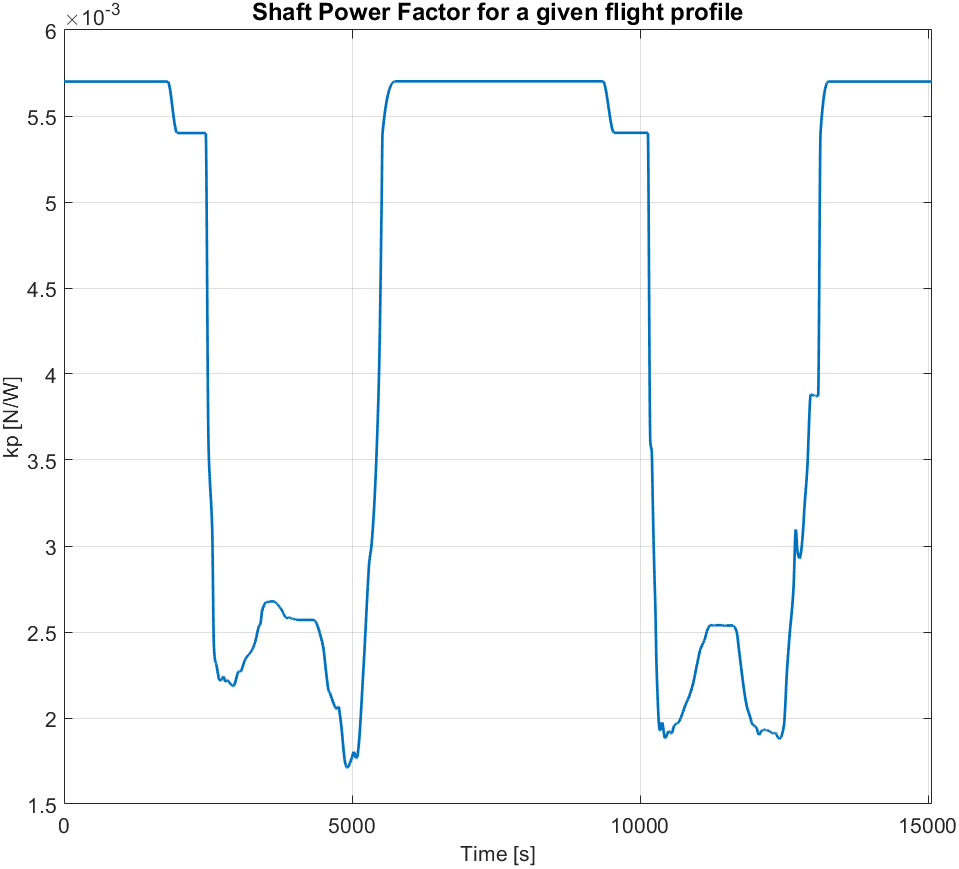
\includegraphics[width=1\textwidth]{Epictures/ShaftPowerFactor.png}
    \caption{Shaft Power Factor for a round trip flight between Copenhagen and Stockholm.}
    \label{fig:ShaftPowerFactor}
\end{figure}


%########################################################################################
\cleardoublepage
\chapter{Miscellaneous loads}
\label{ch:miscloads}
\todo[inline, backgroundcolor=aqua]{Show all other loads, described by previous work.}

%########################################################################################
%\cleardoublepage
\section{Airliner Subsystems}
\label{sec:AirlinerSubsystems}

\todo[inline, backgroundcolor=aqua]{Describe a typical airliner with most subsystems. The energy flow from the engines to the subsystems. Differences with MEA.}
\todo[inline, backgroundcolor=aqua]{Include pictures.}

%########################################################################################

\section{Load comparison}
\label{sec:loadcomp}
\todo[inline, backgroundcolor=aqua]{Compare all kinds of loads (fuel consumption with pie charts), to see how they relates to one another.}


%########################################################################################
\cleardoublepage
\chapter{Compare conventional aircraft and MEA}
\label{ch:compconvMEA}
\todo[inline, backgroundcolor=aqua]{Compare fuel efficiency in 3 different units: kg fuel per seat km, litre fuel per seat km, seat km per litre.}
\todo[inline, backgroundcolor=aqua]{Explain differences.}
\todo[inline, backgroundcolor=aqua]{Pros and cons. Also those that are not related to fuel efficiency.}
\todo[inline, backgroundcolor=aqua]{Include graphs.}

\todo[inline, backgroundcolor=aqua]{Mass of Ice in kg}


%########################################################################################
%\cleardoublepage
%\chapter{Pax-scaling effect on fuel consumption}
%\label{ch:paxscaling}
%\todo[inline, backgroundcolor=aqua]{Show how pax-scaling is affecting fuel efficiency.}
%\todo[inline, backgroundcolor=aqua]{Size matter, but not in the expected way. Explain why.}
%\todo[inline, backgroundcolor=aqua]{Include graphs.}


%########################################################################################
\cleardoublepage
\chapter{Results and Objective Analysis}
\label{ch:resultsAndAnalysis}
\todo[inline, backgroundcolor=aqua]{svensk: Resultat och Analys}

\todo[inline]{
Sometimes this is split into two chapters.
Keep in mind: How you are going to evaluate what you have done? What are your metrics?\\
Analysis of your data and proposed solution.
Does this meet the goals which you had when you started?
}
\todo[inline, backgroundcolor=aqua]{Power consumption for IPS}
\todo[inline, backgroundcolor=aqua]{Other Results from FENSAP Simulation}
In this chapter, we present the results and discuss them.

\begin{swedishnotes}
I detta kapitel presenterar vi resultatet och diskutera dem.
\end{swedishnotes}
\todo[inline, backgroundcolor=aqua]{
Ibland delas detta upp i två kapitel.\\
Hur du ska utvärdera vad du har gjort? Vad är din statistik?\\
Analys av data och föreslagen lösning\\
Innebär detta att uppnå de mål som du hade när du började?
}

%\section{Major Sesults}
%\todo[inline, backgroundcolor=aqua]{Huvudsakliga resultat}
\section{ECS Fuel consumption}
\label{sec:ECSFuelResult}
A case study was done with the Airbus A320 and 180 pax on a round trip Copenhagen-Stockholm-Copenhagen on a hot day (30\degree C). Figure \ref{fig:ECSfuelbreakdown} shows a breakdown of the fuel consumption of all 3 \acrshort{ecs} configurations. We can see that the \acrshort{acm} and \acrshort{eacm} are fairly equal in operational efficiency. If we add the effect of weight and drag, then the \acrshort{eacm} becomes an inferior option. However, in this particular case, for the bleed-air driven \acrshort{acm}, there were some moments when the \acrshort{ecs} forced the engines to run at a higher thrust setting than was required by the aircraft. This happened during the majority of the descent. The combination of low ambient pressure, at high altitude, and low thrust setting, resulted in too low bleed pressure from the engines. To maintain normal operation of the \acrshort{acm}, the \acrshort{ecs} then forces the engines to run at a higher thrust setting. If we take this thrust increased fuel consumption into consideration, then the conventional \acrshort{acm} has a clear disadvantage over the electrical options.

% Altitude of descent when ECS forced thrust occur from 11500 m to 4600 m

\begin{figure}[!ht]
    \centering
    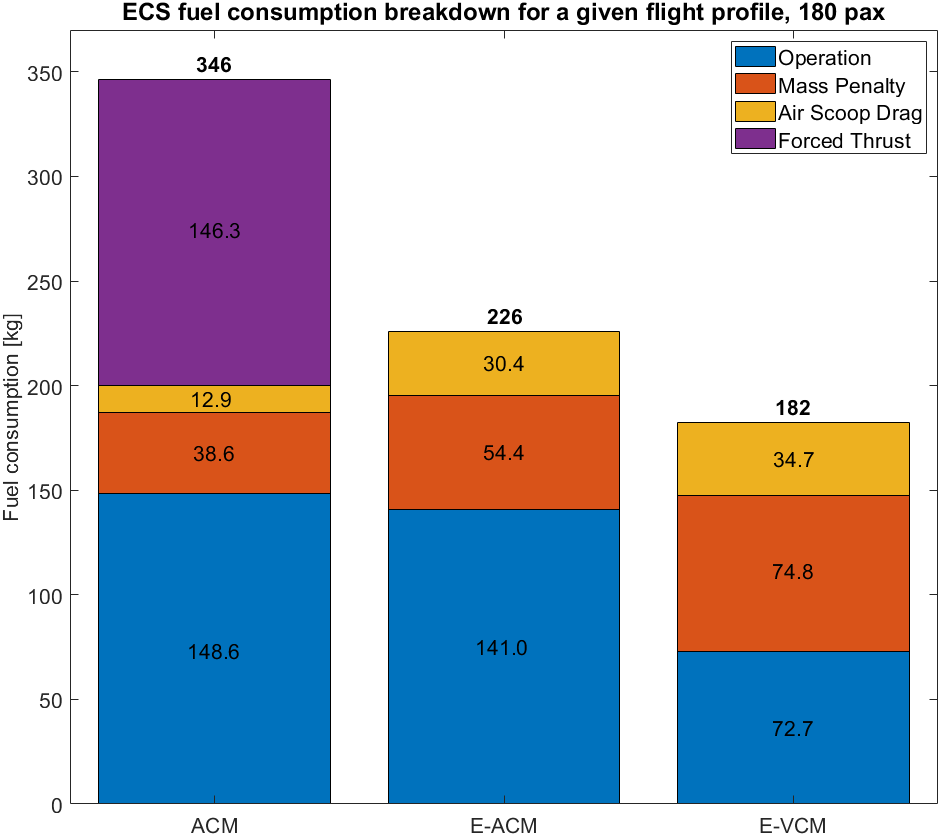
\includegraphics[width=1\textwidth]{Epictures/ECSFuelBreakDown180pax.png}
    \caption{ECS fuel consumption breakdown for a round trip flight, Copenhagen-Stockholm-Copenhagen, with a modelled A320 and 180 pax.}
    \label{fig:ECSfuelbreakdown}
\end{figure}

The \acrshort{vcm} has the most efficient operation, consuming about half the amount of fuel than the \acrshort{acm}. But the weight penalty and increased drag offsets most of the operational efficiency.



\clearpage
\section{ECS Partial Results}
\label{sec:ECSPartResult}

This section will show and discuss significant partial results from a simulation of the case study. Three different airliners were simulated in parallel. They are all based on the same A320 sized aircraft with 180 pax, but with different \acrshort{ecs}, flying on the same path. The flights took place between Copenhagen and Stockholm, back and forth. A hot day (30 \degree C on the ground) was chosen because the heat will stress the \acrshort{ecs} to work harder, magnifying the systems' differences. 

We begin with the Air Mass Flow Rates. Figure \ref{fig:ECSMassFlow} shows air mass flow rates for all 3 systems. When the \acrshort{ecs} is active, the minimum fresh air flow rate for the cabin is $\dot{m}_{air,min}=0.006\cdot 180 = 1.08$ kg/s, otherwise it is zero. During cruise, when not much cooling is required, all systems will run at $\dot{m}_{air,min}$, which can be seen at the purple line. When more cooling is needed at lower altitudes, the flow rates are higher. All three systems use the same amount of fresh air, the dark blue line. As for the cooling air, bleed air from the engine fan, the pre-cooler uses that, is shown in red. Ram air for the \acrshort{acm} heat exchanger is plotted with yellow colour and ram air for the \acrshort{vcm} heat exchangers are shown in green and light blue. The hot side of the \acrshort{vcm} is not allowed to be more than $80\degree$C, which is a relatively low temperature; this explains why the secondary heat exchanger requires much cooling air.

 

\begin{figure}[!ht]
    \centering
    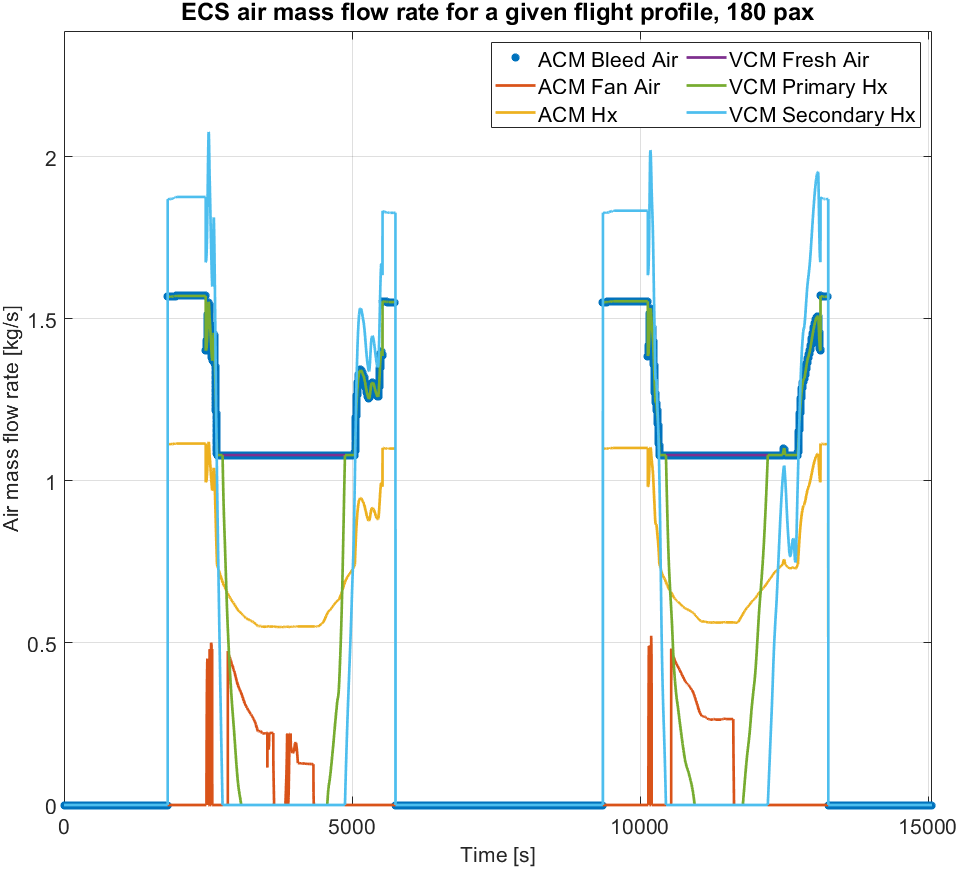
\includegraphics[width=1\textwidth]{Epictures/ECSMassFlow180pax.png}
    \caption{ECS air mass flow rates.}
    \label{fig:ECSMassFlow}
\end{figure}

\clearpage

Compressed air temperature from various parts can be seen in figure \ref{fig:ECSCompTemp}. Each flight begins with the \acrshort{apu} starting up and providing compressed air for the aircraft. Right before taxiing, the engines start and take over the role to provide power for the airliner. This is what we can see as small steps in the graph. During takeoff, the engines are suddenly working much harder, which also increases the bleed air temperature. We can see this as spikes in the graph. A few seconds later, when the \acrshort{lpc} pressure is high enough, switching over from \acrshort{hpc} to \acrshort{lpc} occurs. This explains sudden drops of the bleed temperature.

\begin{figure}[!ht]
    \centering
    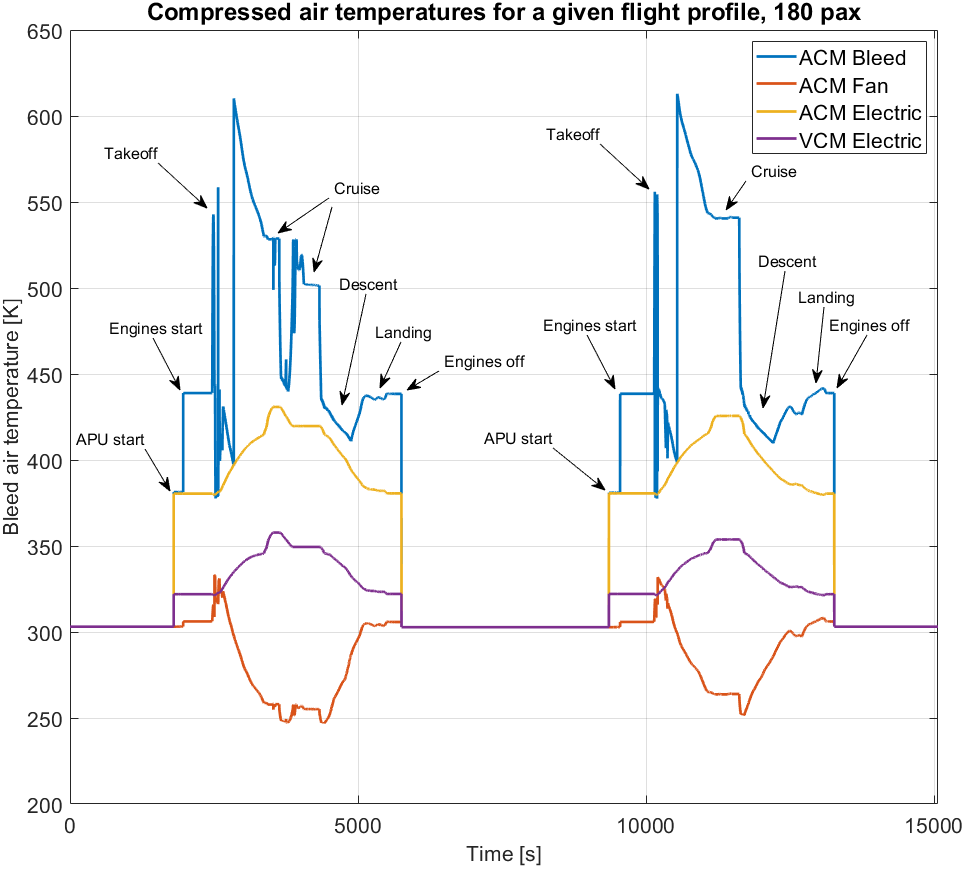
\includegraphics[width=1\textwidth]{Epictures/ECSCompTemp.png}
    \caption{Compressed air temperatures with most of the flight modes.}
    \label{fig:ECSCompTemp}
\end{figure}

\clearpage

Pressure for the bleed ports can be seen in figure \ref{fig:BleedPressure}. About halfway through the climb, the engine's power is low enough for the valves to switch back to HPC and the bleed temperature jumps to a higher level. The bleed temperature is relatively constant during a cruise, except for when the aircraft changes flight level. During descent, the engines are idling or have just enough power to keep the bleed pressure level. For landing, the thrust and temperature increases slightly and continues during the taxi until the aircraft turns off the engines at the gate.

\begin{figure}[!ht]
    \centering
    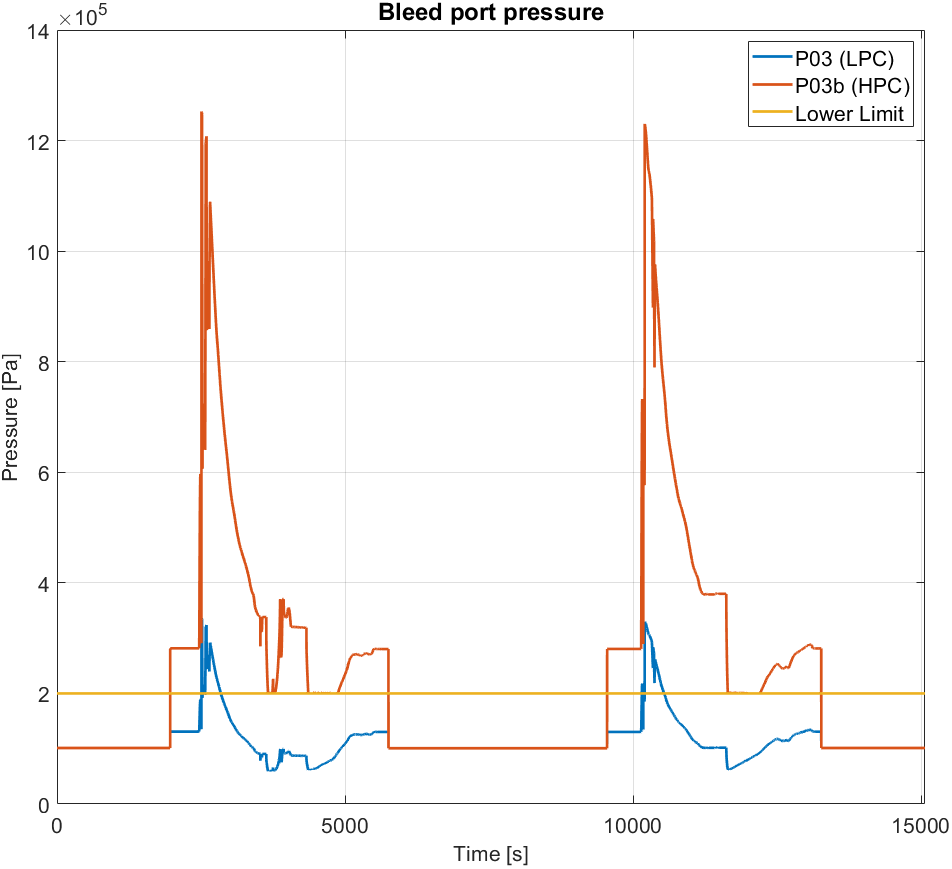
\includegraphics[width=1\textwidth]{Epictures/BleedPortPressure.png}
    \caption{Pressure at the bleed ports.}
    \label{fig:BleedPressure}
\end{figure}

\clearpage

The shaft power to operate the \acrshort{ecs} is shown in figure \ref{fig:ECSShaftPower}, while the fuel consumption can be seen in figure \ref{fig:ECSShaftPowerFuel}. It is interesting to see the transition from \acrshort{apu} to engines fuel consumption in the graph. The fuel consumption steps up for the bleed \acrshort{acm} because bleed air temperature from the engines is higher. But for the electric machines we can see that it steps down, this is explained by the higher efficiency of the engines to generate electricity.

\begin{figure}[!ht]
    \centering
    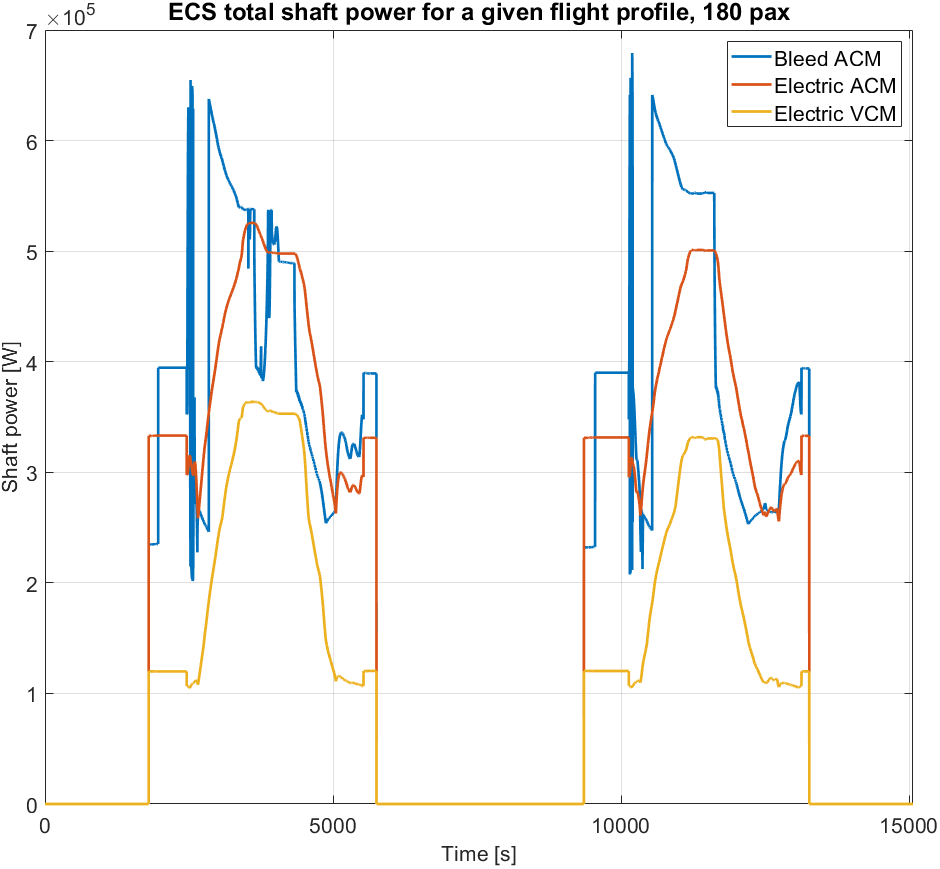
\includegraphics[width=1\textwidth]{Epictures/ECSShaftPower180pax.png}
    \caption{ECS shaft power.}
    \label{fig:ECSShaftPower}
\end{figure}

\begin{figure}[!ht]
    \centering
    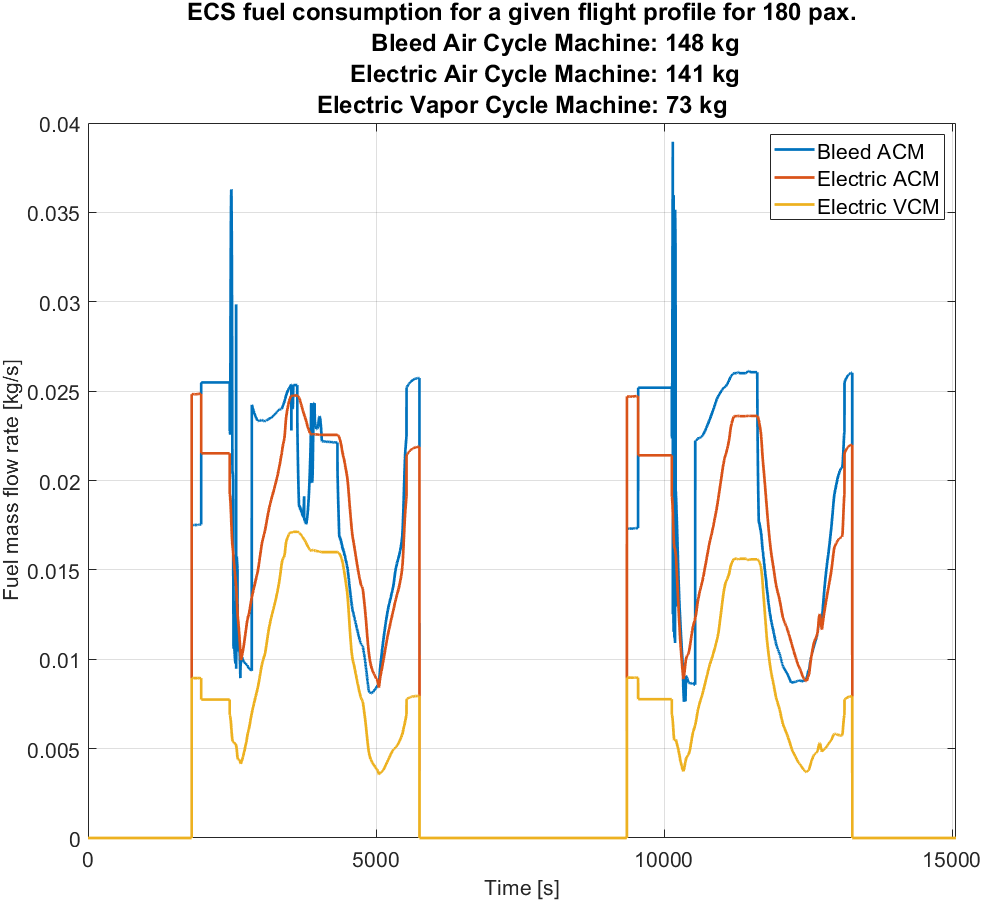
\includegraphics[width=1\textwidth]{Epictures/ECSShaftPowerFuel.png}
    \caption{ECS operational fuel consumption.}
    \label{fig:ECSShaftPowerFuel}
\end{figure}

\clearpage

The fuel consumption to generate thrust is plotted in figure \ref{fig:ThrustFuel180pax}. Here we can see the \acrshort{ecs} thrust increased fuel consumption as the area between the blue and yellow lines.

\begin{figure}[!ht]
    \centering
    \includegraphics[width=1\textwidth]{Epictures/ThrustFuel180pax.png}
    \caption{Fuel consumption due to thrust.}
    \label{fig:ThrustFuel180pax}
\end{figure}


\clearpage
\section{Pax-scaling effect on fuel consumption}
\label{sec:paxscalingeffect}
%\todo[inline, backgroundcolor=aqua]{Show how pax-scaling is affecting fuel consumption.}
%\todo[inline, backgroundcolor=aqua]{Size matter, but not in the expected way. Explain why.}
%\todo[inline, backgroundcolor=aqua]{Include graphs.}
The effect of scaling on fuel consumption was investigated by running several simulations with passenger numbers from 156 to 700 pax. The result was then combined into figures to visualize the trends.
First, we will show the fuel consumption of different \acrshort{ecs}, then for various systems combined. The largest amount of fuel goes to propulsion, thus thrust fuel consumption will be plotted. Lastly, we will display the fuel consumption of the whole aircraft.

The fuel consumption of the bleed air driven \acrshort{ecs} can be seen in figure \ref{fig:ACMFuelCon}. The coloured areas represent different aspects of the \acrshort{ecs} that contribute to fuel consumption. The \acrshort{ecs} it self (ACM Operation + Mass Penalty + Drag Penalty) has a fuel consumption that is nearly independent of scaling, only \textbf{Forced Thrust} seems to be affected by pax-scaling. Since thrust is mostly a function of weight of the aircraft, we can presume that the weight per passenger of the aircraft follows \textbf{Forced Thrust} fuel consumption in the graph.

\begin{figure}[!ht]
    \centering
    \includegraphics[width=1\textwidth]{Epictures/ACMECSfuelCon.png}
    \caption{Conventional \acrshort{ecs} fuel consumption for a round trip flight between Copenhagen and Stockholm.}
    \label{fig:ACMFuelCon}
\end{figure}

\clearpage

Fuel consumption for the \acrshort{eacm} \acrshort{ecs} is shown in figure \ref{fig:EACMFuelCon}. Biggest difference from the conventional version is that \textbf{Forced Thrust} doesn't exist here. Both \textbf{E-ACM Operation} and \textbf{Drag Penalty} are largely unaffected by pax-scaling. \textbf{Mass Penalty} seems to be less with larger passenger count.

\begin{figure}[!ht]
    \centering
    \includegraphics[width=1\textwidth]{Epictures/EACMECSfuelCon.png}
    \caption{\acrshort{eacm} \acrshort{ecs} fuel consumption for a round trip flight between Copenhagen and Stockholm.}
    \label{fig:EACMFuelCon}
\end{figure}

\clearpage

A similar graph is shown For the \acrshort{evcm} \acrshort{ecs}. See figure \ref{fig:EVCMFuelCon}. The trend is that both \textbf{E-VCM Operation} and \textbf{Drag Penalty} are not affected by pax-scaling, while \textbf{Mass Penalty} shows a clear pax dependency.

\begin{figure}[!ht]
    \centering
    \includegraphics[width=1\textwidth]{Epictures/EVCMECSfuelCon.png}
    \caption{\acrshort{evcm} \acrshort{ecs} fuel consumption for a round trip flight between Copenhagen and Stockholm.}
    \label{fig:EVCMFuelCon}
\end{figure}

\clearpage

The effect of pax-scaling on miscellaneous loads can be seen in figure \ref{fig:MiscFuelCon}. Miscellaneous loads are almost the same for all three aircraft. It looks to be varying vastly, but the scaling of the y-axis is miss leading. It changes about 16\% for the whole pax-span.

\begin{figure}[!ht]
    \centering
    \includegraphics[width=1\textwidth]{Epictures/MiscFuelCon.png}
    \caption{Fuel consumption of various loads for a round trip flight between Copenhagen and Stockholm.}
    \label{fig:MiscFuelCon}
\end{figure}

\clearpage

The fuel consumption to generate thrust and its pax-scaling is plotted in figure \ref{fig:ThrustFuelCon}. The conventional aircraft's thrust fuel consumption is around 3\% higher than the \acrshort{mea} alternatives throughout the pax-span. As thrust is mainly a function of weight, these curves' shapes will mostly follow the aircraft mass per passenger. Compare with figure \ref{fig:ZFMppax}.

\begin{figure}[!ht]
    \centering
    \includegraphics[width=1\textwidth]{Epictures/ThrustFuelCon.png}
    \caption{Thrust fuel consumption for a round trip flight between Copenhagen and Stockholm.}
    \label{fig:ThrustFuelCon}
\end{figure}

\begin{figure}[!ht]
    \centering
    \includegraphics[width=1\textwidth]{Epictures/ZFMppax.png}
    \caption{Aircraft Zero Fuel Mass per passenger.}
    \label{fig:ZFMppax}
\end{figure}

\clearpage

By summing up all systems' fuel consumption, we get the fuel consumption of the whole aircraft. See figure \ref{fig:ACFuelCon}. The difference in fuel consumption between the conventional aircraft and the \acrshort{mea} with \acrshort{vcm} is approximately 3\% to 4\%.

The fact that the fuel consumption per passenger and kilometres increases with the aircraft's size seemed counter-intuitive. But if we give it some analytic thoughts, then it becomes obvious why this is the case. Generally, larger airliners are designed to be able to fly at longer distances. It means that they must be able to carry more fuel per passenger (or per payload). As fuel equals weight, it takes more fuel to carry fuel, and it is starting to look like a spiral of fuel increments. More fuel also increases the structural loads, which means that the structure must be stronger. Increased strength usually means more material and mass, and the weight spiral goes on.

\begin{figure}[!ht]
    \centering
    \includegraphics[width=1\textwidth]{Epictures/ACFuelCon.png}
    \caption{Aircraft fuel consumption for a round trip flight between Copenhagen and Stockholm.}
    \label{fig:ACFuelCon}
\end{figure}


\clearpage
\section{Icing Parameters Results}
\subsection{Climb Case Study}
According to the Climb Input parameters enlisted in \ref{tab:climb-table}, two sets of data have been resolved. The first set involves the Rime Type, and the latter one involves the Glaze Advanced type of ice formation.
\subsubsection{Rime Type}
\begin{figure}[!htb]
    \centering
    \includegraphics[width=0.8\textwidth]{IPS/Ice_Shape_Climb_Rime_2D.png}
    \caption{2D View of Rime Ice Shape in Climb Rime Case using ICE3D}
    \label{fig:Ice_Shape_Climb_Rime_2D.png}
\end{figure}
\begin{figure}[!htb]
    \centering
    \includegraphics[width=0.8\textwidth]{IPS/Ice_Shape_Climb_Rime_3D.png}
    \caption{3D View of Rime Ice Shape in Climb Rime Case using ICE3D}
    \label{fig:Ice_Shape_Climb_Rime_3D.png}
\end{figure}
\begin{figure}[!htb]
    \centering
    \includegraphics[width=0.8\textwidth]{IPS/Mass_Caught_Climb_Rime_3D.png}
    \caption{3D View of Mass Caught in Climb Rime Case using ICE3D}
    \label{fig:Ice_Shape_Climb_Rime_3D}
\end{figure}
\begin{figure}[!htb]
    \centering
    \includegraphics[width=0.8\textwidth]{IPS/Mass_Caught_Climb_Rime_2D.png}
    \caption{Mass Caught in Climb Rime Case using ICE3D}
    \label{fig:Ice_Shape_Climb_Rime_2D}
\end{figure}
\begin{figure}[!ht]
    \centering
    \includegraphics[width=0.8\textwidth]{IPS/Ice_Density_Climb_Rime_3D.png}
    \caption{3D View of Ice Density in Climb Rime Case using ICE3D}
    \label{fig:Ice_Density_Climb_Rime_3D}
\end{figure}
\cleardoublepage
\begin{figure}[!htb]
    \centering
    \includegraphics[width=0.8\textwidth]{IPS/Ice_Thickness_Climb_Rime_2D.png}
    \caption{using ICE3D}
    \label{fig:Ice_Thickness_Climb_Rime_2D}
\end{figure}
The colours in the figure \ref{fig:Droplet_Velocity_Magnitude_LWC_DROP3D_Climb_Rime_3D} represent the Droplet Velocity Magnitude.
\begin{figure}[!htb]
    \centering
    \includegraphics[width=0.8\textwidth]{IPS/Droplet_Velocity_Magnitude_LWC_DROP3D_Climb_Rime_3D.png}
    \caption{Droplet Velocity vectors in Climb Rime Case using DROP3D}
    \label{fig:Droplet_Velocity_Magnitude_LWC_DROP3D_Climb_Rime_3D}
\end{figure}

\clearpage
\subsubsection{Glaze Type}
\subsection{Descent Case Study}
According to the Descent Input parameters enlisted in \ref{tab:descent-table}, two sets of data have been resolved. The first set involves the Rime Type, and the latter one involves the Glaze Advanced type of ice formation.

\clearpage
\section{Ice Protection System Results}
%########################################################################################
\clearpage
\subsubsection{\acrfull{pts} Simulation}
%########################################################################################
\clearpage
\subsection{\acrfull{ets} Simulation} 
\clearpage
%################################################
\section{Sensitivity Analysis}
\todo[inline, backgroundcolor=aqua]{Analys av reabilitet}
\begin{swedishnotes}
Reabilitet i metod och data 
\end{swedishnotes}

\section{Validity Analysis}
\todo[inline, backgroundcolor=aqua]{Analys av validitet}
\begin{swedishnotes}
Validitet i metod och data 
\end{swedishnotes}

%########################################################################################
\cleardoublepage
\chapter{Discussion (Subjective Analysis) }
\label{ch:discussion}
\todo[inline]{This can be a separate chapter or a section in the previous chapter.}
\todo[inline, backgroundcolor=aqua]{Discussion}

\begin{swedishnotes}
Förbättringsförslag?
\end{swedishnotes}
Appendix C and \acrshort{sld} do not work together!
%########################################################################################
\cleardoublepage
\chapter{Conclusions and Future work}
\todo[inline, backgroundcolor=aqua]{Slutsats och framtida arbete}
\label{ch:conclusionsAndFutureWork}
Add text to introduce the subsections of this chapter.

\section{Conclusions}
\todo[inline]{Describe the conclusions (reflect on the whole introduction given in Chapter 1).}
\todo[inline, backgroundcolor=aqua]{Slutsatser}
\label{sec:conclusions}
  
Discuss the positive effects and the drawbacks.\\
Describe the evaluation of the results of the degree project.\\
Did you meet your goals?\\
What insights have you gained?\\
What suggestions can you give to others working in this area?\\
If you had it to do again, what would you have done differently?\\

\begin{swedishnotes}
Träffade du dina mål?
Vilka insikter har du fått?
Vilka förslag kan du ge till andra som arbetar inom detta område?
Om du hade att göra igen, vad skulle du ha gjort annorlunda?
\end{swedishnotes}

\section{Limitations}
\todo[inline]{What did you find that limited your
  efforts? What are the limitations of your results?}
\begin{enumerate}
\item Empenage not considered, crystals
\item Only steady state conditions are considered.
\item COWL Ice Protection system (CIPS) not implemented for simulations.
\end{enumerate}
User defined distributions are not yet supported. 
\todo[inline, backgroundcolor=aqua]{Begränsande faktorer}
\label{sec:limitations}
\begin{swedishnotes}
Vad gjorde du som begränsade dina ansträngningar? Vilka är begränsningarna i dina resultat?\\
För IPS
\begin{enumerate}
\item Empennage inte beaktas.
\item Endast stabila tillstånd beaktas.
\item COWL Ice Protection System (CIPS) inte implementerat för simuleringar.
\end{enumerate}
\end{swedishnotes}

\section{Future work}
Workbench Journal Scripting
\todo[inline]{Describe valid future work that you or someone else could or should do.\\
Consider: What you have left undone? What are the next obvious things to be done? What hints can you give to the next person who is going to follow up on your work?
}
\todo[inline, backgroundcolor=aqua]{Vad du har kvar ogjort?\\
Vad är nästa självklara saker som ska göras?\\
Vad tips kan du ge till nästa person som kommer att följa upp på ditt arbete?
}
\label{sec:futureWork}
\todo[inline, backgroundcolor=aqua]{COWL Ice Protection}
Due to the breadth of the problem, only some of the initial goals have been
met. In these section we will focus on some of the remaining issues that
should be addressed in future work. ...

simulink model
\subsection{What has been left undone?}
\label{what-has-been-left-undone}

%The prototype does not address the third requirment, i.e., a yearly
%unavailability of less than 3 minutes, this remains an open problem. ...

%\subsubsection{Cost analysis}
%
%The current prototype works, but the performance from a cost perspective makes
%this an impractical solution. Future work must reduce the cost of this
%solution, to do so a cost analysis needs to first be done. ...
%
%\subsubsection{Security}
%
%A future research effort is needed to address the security holes that results
%from using a self-signed certificate. Page filling text mass. Page filling
%text mass. ...


\subsection{Next obvious things to be done}

In particular, the author of this thesis wishes to point out xxxxxx remains as
a problem to be solved. Solving this problem is the next thing that should be
done. ...

\section{Reflections}
\todo[inline]{What are the relevant economic, social,
  environmental, and ethical aspects of your work?
}
\todo[inline, backgroundcolor=aqua]{Reflektioner}
\todo[inline, backgroundcolor=aqua]{Vilka är de relevanta ekonomiska, sociala, miljömässiga och etiska aspekter av ditt arbete?}
\label{sec:reflections}

%One of the most important results is the reduction in the amount of
%energy required to process each packet while at the same time reducing the
%time required to process each packet.
%
%The thesis contributes to the \gls{UN}\enspace\glspl{SDG} numbers 1 and 9 by
%xxxx. 




\noindent\rule{\textwidth}{0.4mm}
\todo[inline]{In the references, let Zotero or other tool fill this
  in for you. I suggest an extended version of the IEEE  style, to include
  URLs, DOIs, ISBNs, etc., to make it easier for your reader to find
  them. This will make life easier for your opponents and examiner. \\

  IEEE Editorial Style Manual: \url{https://www.ieee.org/content/dam/ieee-org/ieee/web/org/conferences/style_references_manual.pdf}
}
\todo[inline, backgroundcolor=aqua]{Låt Zotero eller annat verktyg fylla i det här för dig. Jag föreslår en utökad version av IEEE stil - att inkludera webbadresser, DOI, ISBN etc. - för att göra det lättare för läsaren att hitta dem. Detta kommer att göra livet lättare för dina motståndare och examinator.}

%########################################################################################
\cleardoublepage
% Print the bibliography (and make it appear in the table of contents)
%\printbibliography[heading=bibintoc]
% The lines below are for BibTeX
\bibliographystyle{myIEEEtran}
\renewcommand{\bibname}{References}
\addcontentsline{toc}{chapter}{References}
\bibliography{references}




%########################################################################################
\cleardoublepage
\appendix
\renewcommand{\chaptermark}[1]{\markboth{Appendix \thechapter\relax:\thinspace\relax#1}{}}
\chapter{Extra material}

\todo[inline, backgroundcolor=aqua]{Show all important input parameters.}
\todo[inline, backgroundcolor=aqua]{Show the MATLAB code.}
%\todo[inline, backgroundcolor=aqua]{svensk: Extra Material som Bilaga}

\section{Miscellaneous Data}
\label{sec:AppMiscData}

\begin{figure}[!ht]
    \centering
    \includegraphics[width=0.7\textwidth]{Epictures/AmbientPressure.png}
    \caption{Ambient pressure profile.}
    \label{fig:Pamb}
\end{figure}

\begin{figure}[!ht]
    \centering
    \includegraphics[width=0.7\textwidth]{Epictures/AmbientTemperature.png}
    \caption{Ambient temperature profile.}
    \label{fig:Tamb}
\end{figure}

\begin{figure}[!ht]
    \centering
    \includegraphics[width=0.7\textwidth]{Epictures/AirDensity.png}
    \caption{Ambient air density profile.}
    \label{fig:Rhoamb}
\end{figure}

\begin{figure}[!ht]
    \centering
    \includegraphics[width=0.7\textwidth]{Epictures/CabinAltitude.png}
    \caption{Cabin altitude. Amended from Hunt et al., 1995, \cite{Hunt1995}}
    \label{fig:CabinAlt}
\end{figure}

\begin{figure}[!ht]
    \centering
    \includegraphics[width=0.7\textwidth]{Epictures/FlightAltitude.png}
    \caption{Altitude profile for the case study.}
    \label{fig:FlightAltitude}
\end{figure}

\begin{figure}[!ht]
    \centering
    \includegraphics[width=0.7\textwidth]{Epictures/VerticalSpeed.png}
    \caption{Vertical speed profile for the case study.}
    \label{fig:VerticalSpeed}
\end{figure}

\begin{figure}[!ht]
    \centering
    \includegraphics[width=0.7\textwidth]{Epictures/VerticalAcceleration.png}
    \caption{Vertical acceleration for the case study.}
    \label{fig:VerticalAcceleration}
\end{figure}

\begin{figure}[!ht]
    \centering
    \includegraphics[width=0.7\textwidth]{Epictures/FlightSpeed.png}
    \caption{Flight speed for the case study.}
    \label{fig:FlightSpeed}
\end{figure}

\begin{figure}[!ht]
    \centering
    \includegraphics[width=0.7\textwidth]{Epictures/FlightAcceleration.png}
    \caption{Flight acceleration for the case study.}
    \label{fig:FlightAcceleration}
\end{figure}

\begin{figure}[!ht]
    \centering
    \includegraphics[width=0.7\textwidth]{Epictures/FlightMode.png}
    \caption{Flight mode for the case study.}
    \label{fig:FlightMode}
\end{figure}

\begin{figure}[!ht]
    \centering
    \includegraphics[width=0.7\textwidth]{Epictures/WingAreavsPax.png}
    \caption{Wing area for the airliners in the study.}
    \label{fig:WingAreaPax}
\end{figure}

\begin{figure}[!ht]
    \centering
    \includegraphics[width=0.7\textwidth]{Epictures/WingChordVSPax.png}
    \caption{Wing mean chord for the airliners in the study.}
    \label{fig:WingChordPax}
\end{figure}

\begin{figure}[!ht]
    \centering
    \includegraphics[width=0.7\textwidth]{Epictures/FuselageLengthVSPax.png}
    \caption{Fuselage effective length for the airliners in the study.}
    \label{fig:FuselageLePax}
\end{figure}

\begin{figure}[!ht]
    \centering
    \includegraphics[width=0.7\textwidth]{Epictures/FuselageDiaVSPax.png}
    \caption{Fuselage diameter for the airliners in the study.}
    \label{fig:FuselageDiaPax}
\end{figure}

\begin{figure}[!ht]
    \centering
    \includegraphics[width=0.7\textwidth]{Epictures/HTailWetVSPax.png}
    \caption{Horizontal tail wet surface area for the airliners in the study.}
    \label{fig:HtailWetPax}
\end{figure}

\begin{figure}[!ht]
    \centering
    \includegraphics[width=0.7\textwidth]{Epictures/HTailChordVSPax.png}
    \caption{Horizontal tail mean chord for the airliners in the study.}
    \label{fig:HtailChordPax}
\end{figure}

\begin{figure}[!ht]
    \centering
    \includegraphics[width=0.7\textwidth]{Epictures/VTailWetVSPax.png}
    \caption{Vertical tail wet surface area for the airliners in the study.}
    \label{fig:VtailWetPax}
\end{figure}

\begin{figure}[!ht]
    \centering
    \includegraphics[width=0.7\textwidth]{Epictures/VtailChordVSPax.png}
    \caption{Vertical tail mean chord for the airliners in the study.}
    \label{fig:VtailChordPax}
\end{figure}

\begin{figure}[!ht]
    \centering
    \includegraphics[width=0.7\textwidth]{Epictures/EnginesDiaSumVSPax.png}
    \caption{Engines diameter sum for the airliners in the study. Pylons surface area is estimated to be proportional to the diameter of the engine by 40\%. }
    \label{fig:EngDiaSumPax}
\end{figure}

\begin{figure}[!ht]
    \centering
    \includegraphics[width=0.7\textwidth]{Epictures/EnginesLengthVSPax.png}
    \caption{Engines effective length for the airliners in the study.}
    \label{fig:EngLePax}
\end{figure}

\begin{figure}[!ht]
    \centering
    \includegraphics[width=0.7\textwidth]{Epictures/WingSweepAngleVSPax.png}
    \caption{Wing quarter chord sweep angle for the airliners in the study.}
    \label{fig:WingSweepPax}
\end{figure}

\begin{figure}[!ht]
    \centering
    \includegraphics[width=0.7\textwidth]{Epictures/McritvsPax.png}
    \caption{Critical Mach number for the airliners in the study.}
    \label{fig:McritPax}
\end{figure}

\begin{figure}[!htb]
    \centering
    \includegraphics[width=1\textwidth]{IPS/cant read ansys mesh.png}
    \caption{Gmsh unable to read mesh generated using ANSYS Mesh.}
    \label{fig:gmsh_error_ansys}
\end{figure}

\begin{figure}[!htb]
    \centering
    \includegraphics[width=1\textwidth]{IPS/cant read gmsh mesh.png}
    \caption{ANSYS unable to read mesh generated using Gmsh.}
    \label{fig:ansys_error_gmsh}
\end{figure}


\clearpage
\section{Code}
\label{sec:AppMatlab}

Listing~\ref{lst:codeexample} is showing a code example in MATLAB format.

\begin{lstlisting}[caption={MATLAB Code for Fuel calculations.}, label=lst:codeexample]
% Testing to include MATLAB code in LaTeX
% ####### VCM ECS fuel consumption #######
if mode == 1
    % Power from APU, 2 kg/min for 447 kW (Honeywell 131-9A), Dieter Scholz
    % - An Optiomal APU for Passenger Aircraft, 2015
    E_VCM_Fuel = 7.4571e-8 * shaftpower_VCM_ecs; % [kg/s] Fuel consumption
    % of ECS and circulation fans
elseif mode==2 || mode==9 % Power from main engines on ground
    % [kg/s] Fuel consumption of ECS and circulation fans
    E_VCM_Fuel = kp*tsfc*shaftpower_VCM_ecs + tsfc*(VCM_Dair + ...
                 VCM_Dphx + VCM_Dshx); 
elseif mode>=3 && mode<=8 && LoD(3)~=0 % Flying normally
    % [kg/s] Fuel consumption of ECS circulation fans and weight penalty
    E_VCM_Fuel = kp*tsfc*shaftpower_VCM_ecs + tsfc*(VCM_Dair + ...
                 VCM_Dphx + VCM_Dshx) - ...
                 tsfc*g*(Mass_ECS_Conv - Mass_ECS_E_VCM)/LoD(3);
elseif mode>=3 && mode<=8 && LoD(3)==0% Flying with no lift
    % [kg/s] Fuel consumption of ECS circulation fans
    E_VCM_Fuel = kp*tsfc*shaftpower_VCM_ecs + tsfc*(VCM_Dair + ... 
                 VCM_Dphx + VCM_Dshx); 
else % Statis on ground. Connected to ground power.
    E_VCM_Fuel = 0;
end
\end{lstlisting}

\lstinputlisting[caption={MATLAB Code : Geometry and Mesh Automation using XFoil and Gmsh.}, label=dhruvmatlabcode]{IPS/Dhruv_Part1_rev4_live.M}


\lstinputlisting[caption={Iron Python Code: climb case study}, label=dhruvpythoncode1]{IPS/IronPython1.tex}


\lstinputlisting[caption={Sample Iron Python Code: meshing}, label=dhruvpythoncode2]{IPS/IronPython2.tex}

\clearpage
\section*{For DIVA}
\divainfo{pg:lastPageofPreface}{pg:lastPageofMainmatter}
\end{document}
